\documentclass[twoside,12pt]{Latex/Classes/PhDthesisPSnPDF}
\usepackage{enumitem, kantlipsum}
\usepackage{mathtools}
\usepackage{amssymb}
\usepackage[warn]{textcomp}
\usepackage{amsbsy}
\usepackage{pifont}
\usepackage{numprint}
\usepackage{lscape}
\usepackage{booktabs}
\usepackage{tikz}
\usepackage{notoccite}
\usepackage[export]{adjustbox}
\usepackage[ruled,vlined]{algorithm2e}
\usepackage{amsmath}
\usepackage{threeparttable, tablefootnote}
\usepackage{tabularx}
\usepackage[table]{xcolor}
\usepackage{array}

\DeclarePairedDelimiter\ceil{\lceil}{\rceil}
\DeclarePairedDelimiter\floor{\lfloor}{\rfloor}
\newcommand\scalemath[2]{\scalebox{#1}{\mbox{\ensuremath{\displaystyle #2}}}}
\newcommand{\cmark}{\ding{51}}
\newcommand{\xmark}{\ding{55}}
\newcommand{\ssep}{;}
\newcommand{\RFCOM}{\raisebox{2pt}{\tikz{\draw[-,black!40!black,solid,line width = 0.9pt](0,0) -- (5mm,0);}}}
\newcommand{\RFSM}{\raisebox{2pt}{\tikz{\draw[-,black!40!black,dashed,line width = 0.9pt](0,0) -- (5mm,0);}}}

\newcommand*\circled[1]{\tikz[baseline=(char.base)]{
            \node[shape=circle,draw,inner sep=1pt] (char) {#1};}}

\newcommand\diag[4]{%
  \multicolumn{1}{p{#2}|}{\hskip-\tabcolsep
  $\vcenter{\begin{tikzpicture}[baseline=0,anchor=south west,inner sep=#1]
  \path[use as bounding box] (0,0) rectangle (#2+2\tabcolsep,\baselineskip);
  \node[minimum width={#2+2\tabcolsep},minimum height=\baselineskip+\extrarowheight] (box) {};
  \draw (box.north west) -- (box.south east);
  \node[anchor=south west] at (box.south west) {#3};
  \node[anchor=north east] at (box.north east) {#4};
 \end{tikzpicture}}$\hskip-\tabcolsep}}


%: Macro file for Latex
% Macros help you summarise frequently repeated Latex commands.
% Here, they are placed in an external file /Latex/Macros/MacroFile1.tex
% An macro that you may use frequently is the figuremacro (see introduction.tex)
%---------------------------------------------------------------
% Macros
% version 3 by Igor Ruiz-Agundez 2011
% version 2 by Jakob Suckale 2007
% version 1 by Harish Bhanderi 2002
%---------------------------------------------------------------

% This file contains macros that can be called up from connected TeX files
% It helps to summarise repeated code, e.g. figure insertion (see below).



%---------------------------------------------------------------
% Figures
%---------------------------------------------------------------


% Makes the \InsertFig macro compatible both with one or two columns
\makeatletter
\newlength \figwidth
\if@twocolumn
  \setlength \figwidth {\columnwidth}
\else
  \setlength \figwidth {\textwidth}
\fi
\makeatother

% \InsertFig allows inserting figures
% Parameters
% 1 --> Filename
% 2 --> Label for referencing
% 3 --> Title describing the figure (caption)
% 4 --> Description of the figure
% 5 --> Figure width, range [0,1]. If parameter is left blank the figure size is not change
% 6 --> Any other option for \includegraphics
% Usage:
% \InsertFig{}{}{}{}{}{}
%
\newcommand{\InsertFig}[6]{%
	\ifthenelse{\isempty{#5}}%
	{% if #1 is empty
		\begin{figure}[htbp!]
		\centering
		\includegraphics[#6]{#1}%
		\caption{#3}{\textbf{#4}}
		\label{#2}
		\end{figure}    
	}
	{% if #1 is not empty
		% 20180625 LED: figuras preferentemente en top
		%\begin{figure}[htbp!]		
		\begin{figure}[!t]
		\centering
		\includegraphics[width=#5\figwidth,#6]{#1}%
		\caption{#3}{\textbf{#4}}
		\label{#2}
		\end{figure}
	}
}

%% Simple version of \InsertFig
%\newcommand{\InsertFig}[5]{
%  \begin{figure}[htbp]
%   	\centering
%    \includegraphics[width=#4\textwidth,#5]{#1}%
%    \caption{#3}
%    \label{#2}
%  \end{figure}
%}



% insert a centered figure with caption
% parameters 1:filename, 2:label, 3:title, 
\newcommand{\figuremacro}[3]{
	\begin{figure}[htbp]
		\centering
		\includegraphics[width=1\textwidth]{#1}
		\caption[#3]{\textbf{#3}}
		\label{#2}
	\end{figure}
}


% insert a centered figure with caption and description
% parameters 1:filename, 2:label, 3:title, 4:description
\newcommand{\figuremacroD}[4]{
	\begin{figure}[htbp]
		\centering
		\includegraphics[width=1\textwidth]{#1}
		\caption[#3]{\textbf{#3} - #4}
		\label{#2}
	\end{figure}
}

% insert a centered figure with caption and description AND WIDTH
% parameters 1:filename, 2:label, 3:title, 4:description, 5: textwidth
% textwidth 1 means as text, 0.5 means half the width of the text
\newcommand{\figuremacroDW}[5]{
	\begin{figure}[htbp]
		\centering
		\includegraphics[width=#5\textwidth]{#1}
		\caption[#3]{\textbf{#3} - #4}
		\label{#2}
	\end{figure}
}

% inserts a figure with wrapped around text; only suitable for NARROW figs
% o is for outside on a double paged document; others: l, r, i(inside)
% text and figure will each be half of the document width
% note: long captions often crash with adjacent content; take care
% in general: above 2 macro produce more reliable layout
\newcommand{\figuremacroN}[3]{
	\begin{wrapfigure}{o}{0.5\textwidth}
		\centering
		\includegraphics[width=0.48\textwidth]{#1}
		\caption[#2]{{\small\textbf{#2} - #3}}
		\label{#1}
	\end{wrapfigure}
}




% Estas definiciones son para el comando \InsertFigBox
\newlength{\anchoFigura}
\newlength{\anchoFloat}
\addtolength{\fboxsep}{2\fboxsep}
%\renewcommand{\capfont}{\normalfont\normalcolor\sffamily\small}
%\renewcommand{\caplabelfont}{\normalfont\normalcolor\sffamily\bfseries\small}

% El comando \InsertFigBox nos permite insertar figuras en un marco
% Los parametros son:
% 1 --> Fichero de la imagen
% 2 --> Etiqueta (label) para referencias
% 3 --> Texto a pie de imagen
% 4 -> Porcentaje del ancho de página que ocupará la figura (de 0 a 1)
% 5 --> Opciones que queramos pasarle al \includegraphics
\newcommand{\InsertFigBox}[5]{%
  \setlength{\anchoFloat}{#4\textwidth}%
  \addtolength{\anchoFloat}{-4\fboxsep}%
  \setlength{\anchoFigura}{\anchoFloat}%
  \begin{figure}%
    \begin{center}%
      \Ovalbox{%
        \begin{minipage}{\anchoFloat}%
          \begin{center}%
            \includegraphics[width=\anchoFigura,#5]{#1}%
            \caption{#3}%
            \label{#2}%
          \end{center}%
        \end{minipage}
      }%
    \end{center}%
  \end{figure}%
}



%---------------------------------------------------------------
% Misc
%---------------------------------------------------------------

% predefined commands by Harish
\newcommand{\PdfPsText}[2]{
  \ifpdf
     #1
  \else
     #2
  \fi
}


%---------------------------------------------------------------
% Locales
%---------------------------------------------------------------


%%
%% Para quitar traducciones raras (Cuadros)
%% A de usarse cada vez que se seleccione el idioma
%%
\newcommand{\MejorarTraducciones}{%
       \renewcommand{\listtablename}{Índice de tablas}
       \renewcommand{\tablename}{Tabla}
       \renewcommand{\lstlistingname}{Lista}
}%



%---------------------------------------------------------------
% Source code
%---------------------------------------------------------------


%%
%% Para escribir extractos de codigo
%%
%% Las tabulaciones se substituyen por dos espacios
%\fvset{tabsize=2}
%% Creamos un nuevo environment de fancyvrb para los ejemplos enmarcados
%\DefineVerbatimEnvironment{VerbEj}{BVerbatim}{fontsize=\small,samepage=true,commandchars=\\\{\}}
%% Colo de fondo
%\definecolor{grisfondo}{gray}{0.9}
%% Environment para extractos de codigo
%\newenvironment{codigo}%
%{\VerbatimEnvironment\begin{Sbox}\begin{VerbEj}}%
%{\end{VerbEj}\end{Sbox}\setlength{\fboxsep}{8pt}\begin{center}\fcolorbox{black}{grisfondo}{\TheSbox}\end{center}}
%
%% Otro formato más bonito para código fuente
%\newcommand{\codigofuente}[3]{%
%  \lstinputlisting[language=#1,caption={#2}]{#3}%
%}





%: ----------------------------------------------------------------------
%:                  TITLE PAGE: name, degree,..
% ----------------------------------------------------------------------
% 201803015 LED: I create some metadata to have a unique source for these fields
\def\myauthor{Ahmed Hamdy Madkour} % Author
%\def\mytitle{Pedestrian Localization using Wrist-Worn Smart Devices} % title
\def\mytitle{Learning in Non-stationary Envioronment } % title
\def\myadvisor{Dr. Amgad Monir and Prof. Hatem Mohamed} % Supervisor

% if output to PDF then put the following in PDF header
\ifpdf
    \pdfinfo { /Title  (\mytitle)
               /Creator (TeX)
               /Producer (pdfTeX)
               /Author (\myauthor)
               /CreationDate (D:201803150940)  %format D:YYYYMMDDhhmmss
               /ModDate (D:YYYYMMDDhhmm)
               /Subject (Pedestrian Localization)
               /Keywords (Auto machine learning, Concept drift, Imbalanced Stream, Transfer Learning, Emerging new Classes, and Dynamic Ensemble Selection.) }
    \pdfcatalog { /PageMode (/UseOutlines)
                  /OpenAction (fitbh)  }
    % 201803015 LED: \pdfinfo does not work in combination with hyperref
    \hypersetup{
    	pdfinfo={
    			Title={\mytitle},
                Author={\myauthor},
                Creator={TeX},
                Producer={pdfTeX},
                CreationDate={D:201803150940},
                ModDate={D:\pdfdate},
                Subject={Transportation},
                Keywords={Auto machine learning, Concept drift, Imbalanced Stream, Transfer Learning, Emerging new Classes, and Dynamic Ensemble Selection.}
    	}
}
\fi

% below is to generate the title page with crest and author name

% Title of the dissertation
%\title{Pedestrian Localization using Wrist-Worn Smart Devices}
\title{\mytitle}
\author{\myauthor}
\advisor{\myadvisor}

% ----------------------------------------------------------------------
% This section below defines front covert (external and internal)
% Shield logo
%\crest{
\includegraphics[width=2cm]{Deusto_Shield}}
\crest{
\includegraphics[width=2cm]{faculty_image.png}}
% \crest{
\includegraphics[width=2cm]{menoufia_logo.png}}
% Full logo
%\crest{
\includegraphics[width=6cm]{UDeusto}}
\university{Menoufia University}
\degree{A dissertation submitted in partial fulfillment of the requirements for the Doctor of Philosophy degree, Faculty of Computers and Information, Menoufia University}
\textadvisor{Supervised by }
\textsignaturecandidate{The candidate}
\textsignatureadvisor{The supervisor}
\cityofbirth{Menoufia}
\degreedate{\monthname \ \the\year}
%\degreedate{Month de \the\year}


% ----------------------------------------------------------------------

% turn of those nasty overfull and underfull hboxes
\hbadness=10000
\hfuzz=50pt



\begin{document}

%\selectlanguage{british}
\selectlanguage{english}

% sets line spacing
\renewcommand\baselinestretch{1.2}
\baselineskip=18pt plus1pt

% Watermark
%\watermark{DRAFT	DRAFT	DRAFT	DRAFT	DRAFT	DRAFT	DRAFT	DRAFT	DRAFT}


% Custom command to format text with two images in between and captions

\begin{titlepage}
    \begin{tabbing}
        \hspace{1cm} % Adjust this to control the space on the left side
        \= \kill % Set tab stops
        \begin{tabular}{ccc} % 3 columns with space between them
          
\includegraphics[width=3cm]{0_frontmatter/figures/PNG/faculty_image.png} & \hspace{2.5cm} & 
\includegraphics[width=3cm]{0_frontmatter/figures/PNG/menoufia_logo.png} \\
          \multicolumn{1}{l}{Faculty of Computer and Information} & \hspace{2.5cm}  & \multicolumn{1}{l}{Menoufia  University} \\
        \end{tabular}\\
    \end{tabbing}
    \begin{center}
        \vspace{0.5cm}

        \textbf{\Huge \normalfont Learning in Nonstationary Environment:Concept Drift handling techniques} 
        \vspace{0.6cm}
        
        \textbf{\large \normalfont A thesis submitted to the Faculty of Computers and Information, Menoufia University, in partial fulfillment of the requirements for the degree of Master of Computers and Information} \\
        \vspace{0.4cm}
        
        \textbf{\large In} \\
        \vspace{0.3cm}
        
        \textbf{\Large [Information Systems]} \\
        \vspace{0.6cm}
        
        \textbf{\Large By} \\
        \vspace{0.3cm}
        
        \textbf{\LARGE  Ahmed Hamdy Madkour} \\
        \vspace{0.3cm}
        
        \textbf{\large \normalfont Teaching Assessment at Information Systems Department, Faculty of Computers and Information, Menoufia University} \\
        \vspace{0.7cm}
        
        \textbf{\Large Supervised By} \\

    \begin{tabbing}
        \hspace{1cm} % Adjust this to control the space on the left side
        \= \kill % Set tab stops
        \begin{tabular}{ccc} % 3 columns with space between them
            \textbf{Prof. Hatem Mohamed} && \textbf{Dr. Amgad Monir} \\
            Professor of Information Systems,  && Lecturer of Information Systems,\\
             Dean for Faculty of Computers and &&  Faculty of Computers and Information,
            \\
            Information, Menoufia University  && Menoufia University \\\\
            \hspace{0.1cm} [ \hspace{3.5cm} ] && \hspace{0.1cm} [ \hspace{3.5cm} ]
        \end{tabular}
    \end{tabbing}
    \vspace{0.4cm}
    \textbf{\Large 2024} 
    \end{center}
\end{titlepage}


% Custom command to format text with two images in between and captions

\begin{titlepage}
	\begin{tabbing}
		\hspace{1cm} % Adjust this to control the space on the left side
		\= \kill % Set tab stops
		\begin{tabular}{ccc} % 3 columns with space between them
			
\includegraphics[width=3cm]{0_frontmatter/figures/PNG/faculty_image.png} & \hspace{2.5cm} & 
\includegraphics[width=3cm]{0_frontmatter/figures/PNG/menoufia_logo.png} \\
			\multicolumn{1}{l}{Faculty of Computer and Information}                  & \hspace{2.5cm} & \multicolumn{1}{l}{Menoufia  University}                                 \\
		\end{tabular}
	\end{tabbing}
	\begin{center}
		\vspace{0.5cm}

		\textbf{\Huge \normalfont Learning in No Stationary Environment: Concept Drift Handling Techniques}
		\vspace{0.3cm}

		\textbf{\large \normalfont A thesis submitted to the Faculty of Computers and Information, Menoufia University, in partial fulfillment of the requirements for the degree of Master of Computers and Information} \\
		\vspace{0.2cm}

		\textbf{\large In} \\
		\vspace{0.2cm}

		\textbf{\Large [Information Systems]} \\
		\vspace{0.5cm}

		\textbf{\Large By} \\
		\vspace{0.3cm}

		\textbf{\LARGE  Ahmed Hamdy Madkour} \\
		\vspace{0.1cm}

		\textbf{\large \normalfont Teaching Assessment at Information Systems Department, Faculty of Computers and Information, Menoufia University} \\
		\vspace{0.5cm}

		\textbf{\Large Examination Committee}
		\vspace{0.0cm}

		\begin{tabbing}
			\begin{tabular}{ccc} % 3 columns with space between them
				\textbf{Prof. Hatem Mohamed}      &  & \textbf{Prof. Hatem Mohamed}              \\
				Professor of Information Systems,  &  & Professor of Information Systems,      \\
				Dean for Faculty of Computers and &  & Faculty of Computers and Information,
				\\
				Information, Menoufia University  &  & Menoufia University                   \\
				\hspace{0.1cm} [ \hspace{3.5cm} ] &  & \hspace{0.1cm} [ \hspace{3.5cm} ]\\
			\end{tabular}
		\end{tabbing}
		

        \begin{center} % Center the entire block on the page
            \begin{tabbing}
                \begin{tabular}{ccc} % Single column with centered content
                  \hspace{3cm}  &\textbf{Prof. Hatem Mohamed} &\\
                    & LProfessor of Information Systems, &\\
                    & Faculty of Computers and Information, &\\
                    & Menoufia University &\\
                    & \hspace{0.1cm} [ \hspace{3.5cm} ]&
                \end{tabular}
            \end{tabbing}
        \end{center}

		\vspace{0.2cm}
		\textbf{\Large 2024}

	\end{center}
\end{titlepage}



% The frontmatter text starts here
\frontmatter


% Thesis Abstract -----------------------------------------------------


%\begin{abstractslong}    %uncommenting this line, gives a different abstract heading


\begin{alwayssingle} \pagestyle{empty}\begin{center}
    \vspace*{1.5cm}
    {\Large \bfseries  Abstract}
  \end{center}      %this creates the heading for the abstract page
    This thesis addresses challenges in machine learning models when dealing with multi-class imbalanced data streams in non-stationary environments. These challenges result in biases, unreliable predictions, and diminished model performance. To overcome these issues, the thesis introduces innovative approaches that combines Dynamic Ensemble Selection (DES) technique, an adaptive method for handling imbalanced multi-class data streams, a concept drift detector, eigen vector technique, and the K-Nearest Neighbors (KNN) algorithm to address class overlap.
    The main objective is to improve the classification of imbalanced multi-class drifted data streams. The adaptive oversampling method generates synthetic samples to mitigate imbalanced data stream issues, with KNN ensuring non-overlapping generated samples. A drift detector assists in deciding whether to keep existing classifiers or create new ones to handle incoming data streams. Dynamic Ensemble Selection (DES) optimizes the classification task by selecting the most appropriate classifier for incoming data. The proposed method offers an effective solution for achieving accurate and resilient classification in the context of imbalanced multi-class drifted data streams. 
    Additionally, the thesis discusses challenges posed by emerging new classes in dynamic data streams for incremental learning. Existing approaches struggle with high false positive rates, long prediction times, and the impractical assumption of having access to true labels for all instances when new classes emerge. To address these challenges, the thesis proposes a novel framework that integrates concept drift detection using the ADWIN method and ensemble stratified bagging. By leveraging true labels during the learning process, the framework effectively detects concept drifts and adapts to accommodate emerging new classes. 
    Furthermore, the thesis discusses challenges faced by machine learning models in heterogeneous multisource streams and non-stationary conditions, which can introduce biases and unreliable predictions. In response, the thesis introduces a comprehensive framework that combines dynamic ensemble selection, eigenvector techniques, and a concept drift detector to enhance transfer learning of multi-class data streams subject to drift. During the training phase, the proposed weighted method assigns appropriate weights to each classifier, mitigating adverse learning effects. Eigenvectors handle heterogeneous multisource streams, and Dynamic Ensemble Selection (DES) determines the most fitting classifiers for incoming data. A concept drift detector identifies and addresses drifted chunks within the data stream.
    The experimental results on various datasets, encompassing benchmark datasets, a real application stream dataset, and synthetic data streams, consistently demonstrate the superior performance of the proposed approach in effectively addressing challenges inherent in such dynamic data streams. Through evaluations conducted on both real-world and synthetic datasets, the framework exhibits exceptional accuracy, precision, recall, geometric mean, and F1-measure, all while maintaining an efficient runtime.
    This robust performance positions the proposed approach as a frontrunner in enabling incremental learning within real-time scenarios, particularly in the context of emerging new classes. The framework provides a comprehensive solution to the intricate complexities associated with incremental learning in dynamic data streams. Moreover, the experimental findings underscore the efficacy and superiority of the proposed approach, particularly when confronted with the unique challenges posed by imbalanced drifted streams, emerging new classes, and heterogeneous multisource drifted data streams.
    Comparisons against state-of-the-art chunk-based methods consistently highlight the effectiveness of this approach in successfully managing the complexities inherent in these multifaceted data stream challenges. In essence, the proposed approach stands out as a powerful and versatile solution, showcasing its ability to outperform existing methods and addressing the evolving demands of imbalanced drifted streams and heterogeneous multisource streams.\\
    \emph{\textbf{Keywords:} Auto machine learning, Concept drift, Imbalanced Stream, Transfer Learning, Emerging new Classes, and Dynamic Ensemble Selection.}
    
\end{alwayssingle}

% \begin{resumen}        %this creates the heading for the abstract page
%\selectlanguage{spanish}
% Motivación

% \end{resumen}


%\begin{laburpena}        %this creates the heading for the abstract page
%\selectlanguage{basque}
%% Jarri zure laburpena hemen.
%%
%
%
%\end{laburpena}

%\end{abstractlongs}


% ----------------------------------------------------------------------

\begin{alwayssingle} \pagestyle{empty}\begin{center}
    \vspace*{1.5cm}
    {\Large \bfseries  Summary}
  \end{center}       %this creates the heading for the abstract page
The thesis proposes three innovative solutions to challenges faced by machine learning models in handling multi-class imbalanced data streams, emerging new classes, and heterogeneous muti-class streams in non-stationary environments. The primary issues include bias, unreliable predictions, and decreased overall model performance.
The first proposed approach integrates the Dynamic Ensemble Selection (DES), an adaptive oversampling method for handling imbalanced multi-class data streams, a concept drift detector, and the K-Nearest Neighbors (KNN) algorithm to address class overlap. The adaptive oversampling method generates synthetic samples, leveraging KNN to ensure non-overlapping samples. A drift detector helps decide whether to keep existing classifiers or create new ones for incoming data streams. Dynamic Ensemble Selection optimizes classifier performance. The approach demonstrates effectiveness in achieving accurate and resilient classification in imbalanced multi-class drifted data streams, as validated through experiments on various datasets.
Similarly, the second paper addresses the challenge of emerging new classes in dynamic data streams, affecting incremental learning. The second proposed approach integrates concept drift detection using the ADWIN method and ensemble stratified bagging. Leveraging true labels during the learning process, this approach detects concept drifts and adapts to emerging new classes. Evaluation using real and synthetic datasets shows superiority in accuracy, precision, recall, geometric mean, and F1 measure while maintaining efficient runtime. The framework promises to enable incremental learning in real-time scenarios, offering a comprehensive solution by combining concept drift detection (ADWIN) and ensemble stratified bagging.
Lastly, the third approach tackles challenges arising from heterogeneous multisource streams and non-stationary conditions in machine learning models. The third proposed approach combines DES, eigen vector techniques, and a concept drift detector to enhance transfer learning of multi-class data streams subject to drift. The weighted method assigns appropriate weights to each classifier during training, mitigating adverse learning effects. Eigenvectors handle heterogeneous multisource streams, and DES determines fitting classifiers for incoming data. The concept drift detector identifies and addresses drifted chunks within the data stream. Experiments on various datasets demonstrate the efficacy and superiority of the proposed approach in addressing challenges presented by transfer learning from heterogeneous multi-sources and concept drift, outperforming state-of-the-art chunk-based methods.

\end{alwayssingle}


% ----------------------------------------------------------------------

% Thesis Acknowledgements ------------------------------------------------


% Opening of the acknowledgements

%Short version
%this creates the heading for the acknowlegments
\begin{acknowledgements}
    First and foremost, I give my deep thanks to Allah for giving me the opportunity and the strength to accomplish this work.



    I would like to thank my supervisors Dr. Hatem Mohammed and Dr. Amgad Monir for their help and support during my work for creating a very inspiring research environment. They have been helpful with background information and have continually encouraged me and helped me with comments on my work. They always had time to discuss new ideas and give feedback on early ideas and research problems.
    
    I would like to thank my family who was a constant source of rising and supporting my spirit. Thanks go out especially to my father, my mother, my wife, and my brothers for support and encouragement.
    
    Finally, special thanks to my faculty, department, and my colleagues.
    
\begin{flushright}
\textit{Thank you everyone,}

Ahmed Madkour

% Moth and year
\monthname \ \the\year



% Signature figure

%\begin{figure}[htbp!]
%\end{figure}
%\includegraphics{signature}%



\end{flushright}



%Closing of the acknowledgements
%Short version
\end{acknowledgements}
% Long version
%\end{acknowledgementslong}

% ------------------------------------------------------------------------




% As abstract contains various languages we set the main language again
%\selectlanguage{british}
\selectlanguage{english}


%: ----------------------- contents ------------------------

\setcounter{secnumdepth}{5} % organisational level that receives a numbers
\setcounter{tocdepth}{5}    % print table of contents for level 3

\tableofcontents 
\listoffigures	% print list of figures
\listoftables  % print list of tables
\listofalgocfs
\printnomenclature % [] = distance between entry and description

\label{sec:glossary} % target name for links to glossary

\mainmatter
\pagestyle{fancy}


% =======================[chapters]=======================
% introduction

% this file is called up by thesis.tex
% content in this file will be fed into the main document


% this file is called up by thesis.tex
% content in this file will be fed into the main document

%: ----------------------- introduction file header -----------------------


\begin{savequote}[50mm]
Success is the sum of small efforts, repeated day-in and day-out.
\qauthor{Robert Collier}
\end{savequote}

\chapter{Introduction}
\label{cha:1_Introduction}

% the code below specifies where the figures are stored
\ifpdf
    \graphicspath{{1_introduction/figures/PNG/}{1_introduction/figures/PDF/}{1_introduction/figures/}}
\else
    \graphicspath{{1_introduction/figures/EPS/}{1_introduction/figures/}}
\fi


%-------------------------------------------------------------------------
%Chapter 1 contents:
%- Motivation of the research field: Context-aware systems -> LBS -> GNSS limitation -> Positioning techniques -> DR -> inertial PDR -> inertial PDR + wearables
%- Problem identification: smartphone not a wearable -> potentiality of wrist-worn wearables -> Problem: no wrist-worn PDRS
%- Goal of the thesis: tackle the problem -> how? Splitting it into sub-problems
%- Structure of the thesis
%-------------------------------------------------------------------------

Governments and companies are producing vast streams of data and require effective data analytics and machine learning methods to assist in making predictions and decisions promptly. One crucial aspect is the machine learning pipeline, which involves training a prepared dataset to construct a model and subsequently utilizing this model to predict new instance outputs. As depicted in Fig. \ref{fig:machine-old-senario}, the process entails fetching historical data from the database during the training phase to construct the machine learning model. Then, the system can input new instances from the database to predict the output.

\begin{figure}[!ht]
    \centering
    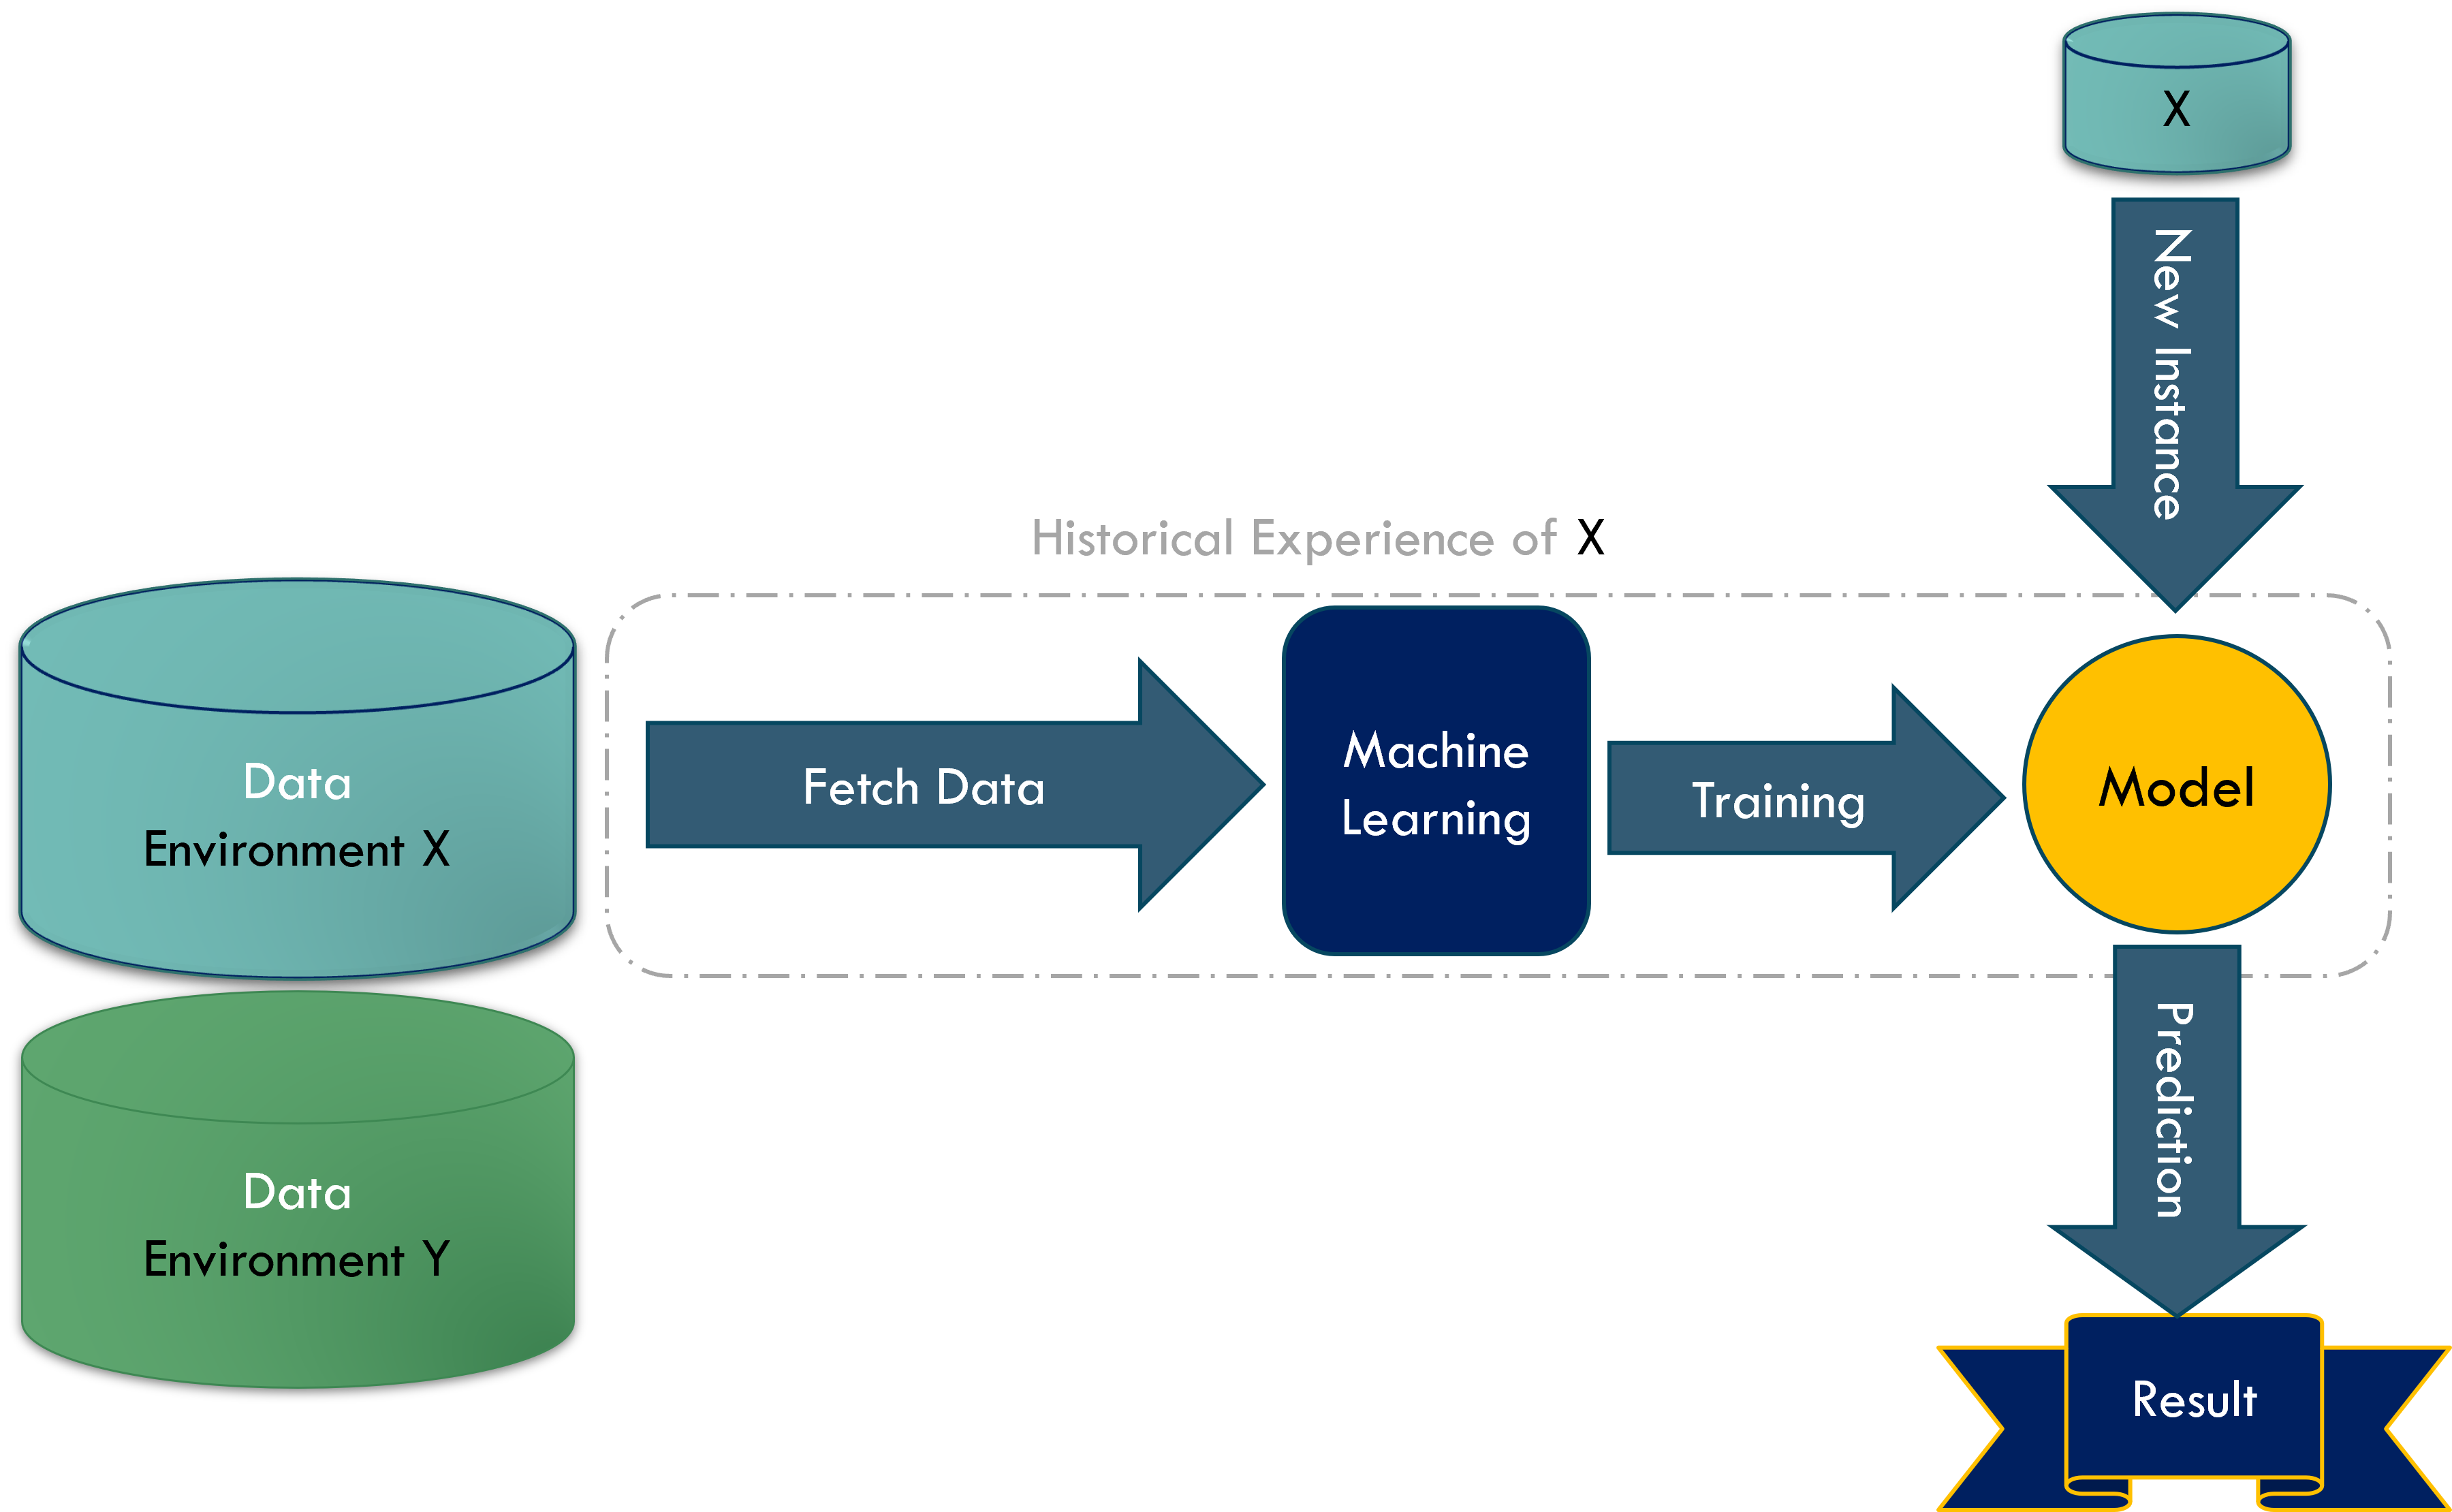
\includegraphics[width=.9\textwidth]{1_introduction/figures/PNG/machine_flow.png}
    \caption{The research methodology of the thesis.}
    \label{fig:machine-old-senario}
\end{figure}

Nevertheless, when endeavoring to forecast outcomes for fresh instances sourced from an alternative database, as illustrated in Fig. \ref{fig:machine-new-senario}
, there frequently emerges a conspicuous decline in accuracy. This disparity accentuates the imperative for model developers to intervene and rectify the issue. Addressing this, developers must adjust and retrain the model utilizing datasets from the new environment to ameliorate accuracy. This iterative process aims to refine the model's precision and ensure its efficacy across diverse contexts, thereby bolstering the reliability of decision-making and predictive capabilities. To confront this challenge, the field of auto machine learning endeavors to facilitate online updates to the model without necessitating direct intervention from developers for modification.

\begin{figure}[!ht]
    \centering
    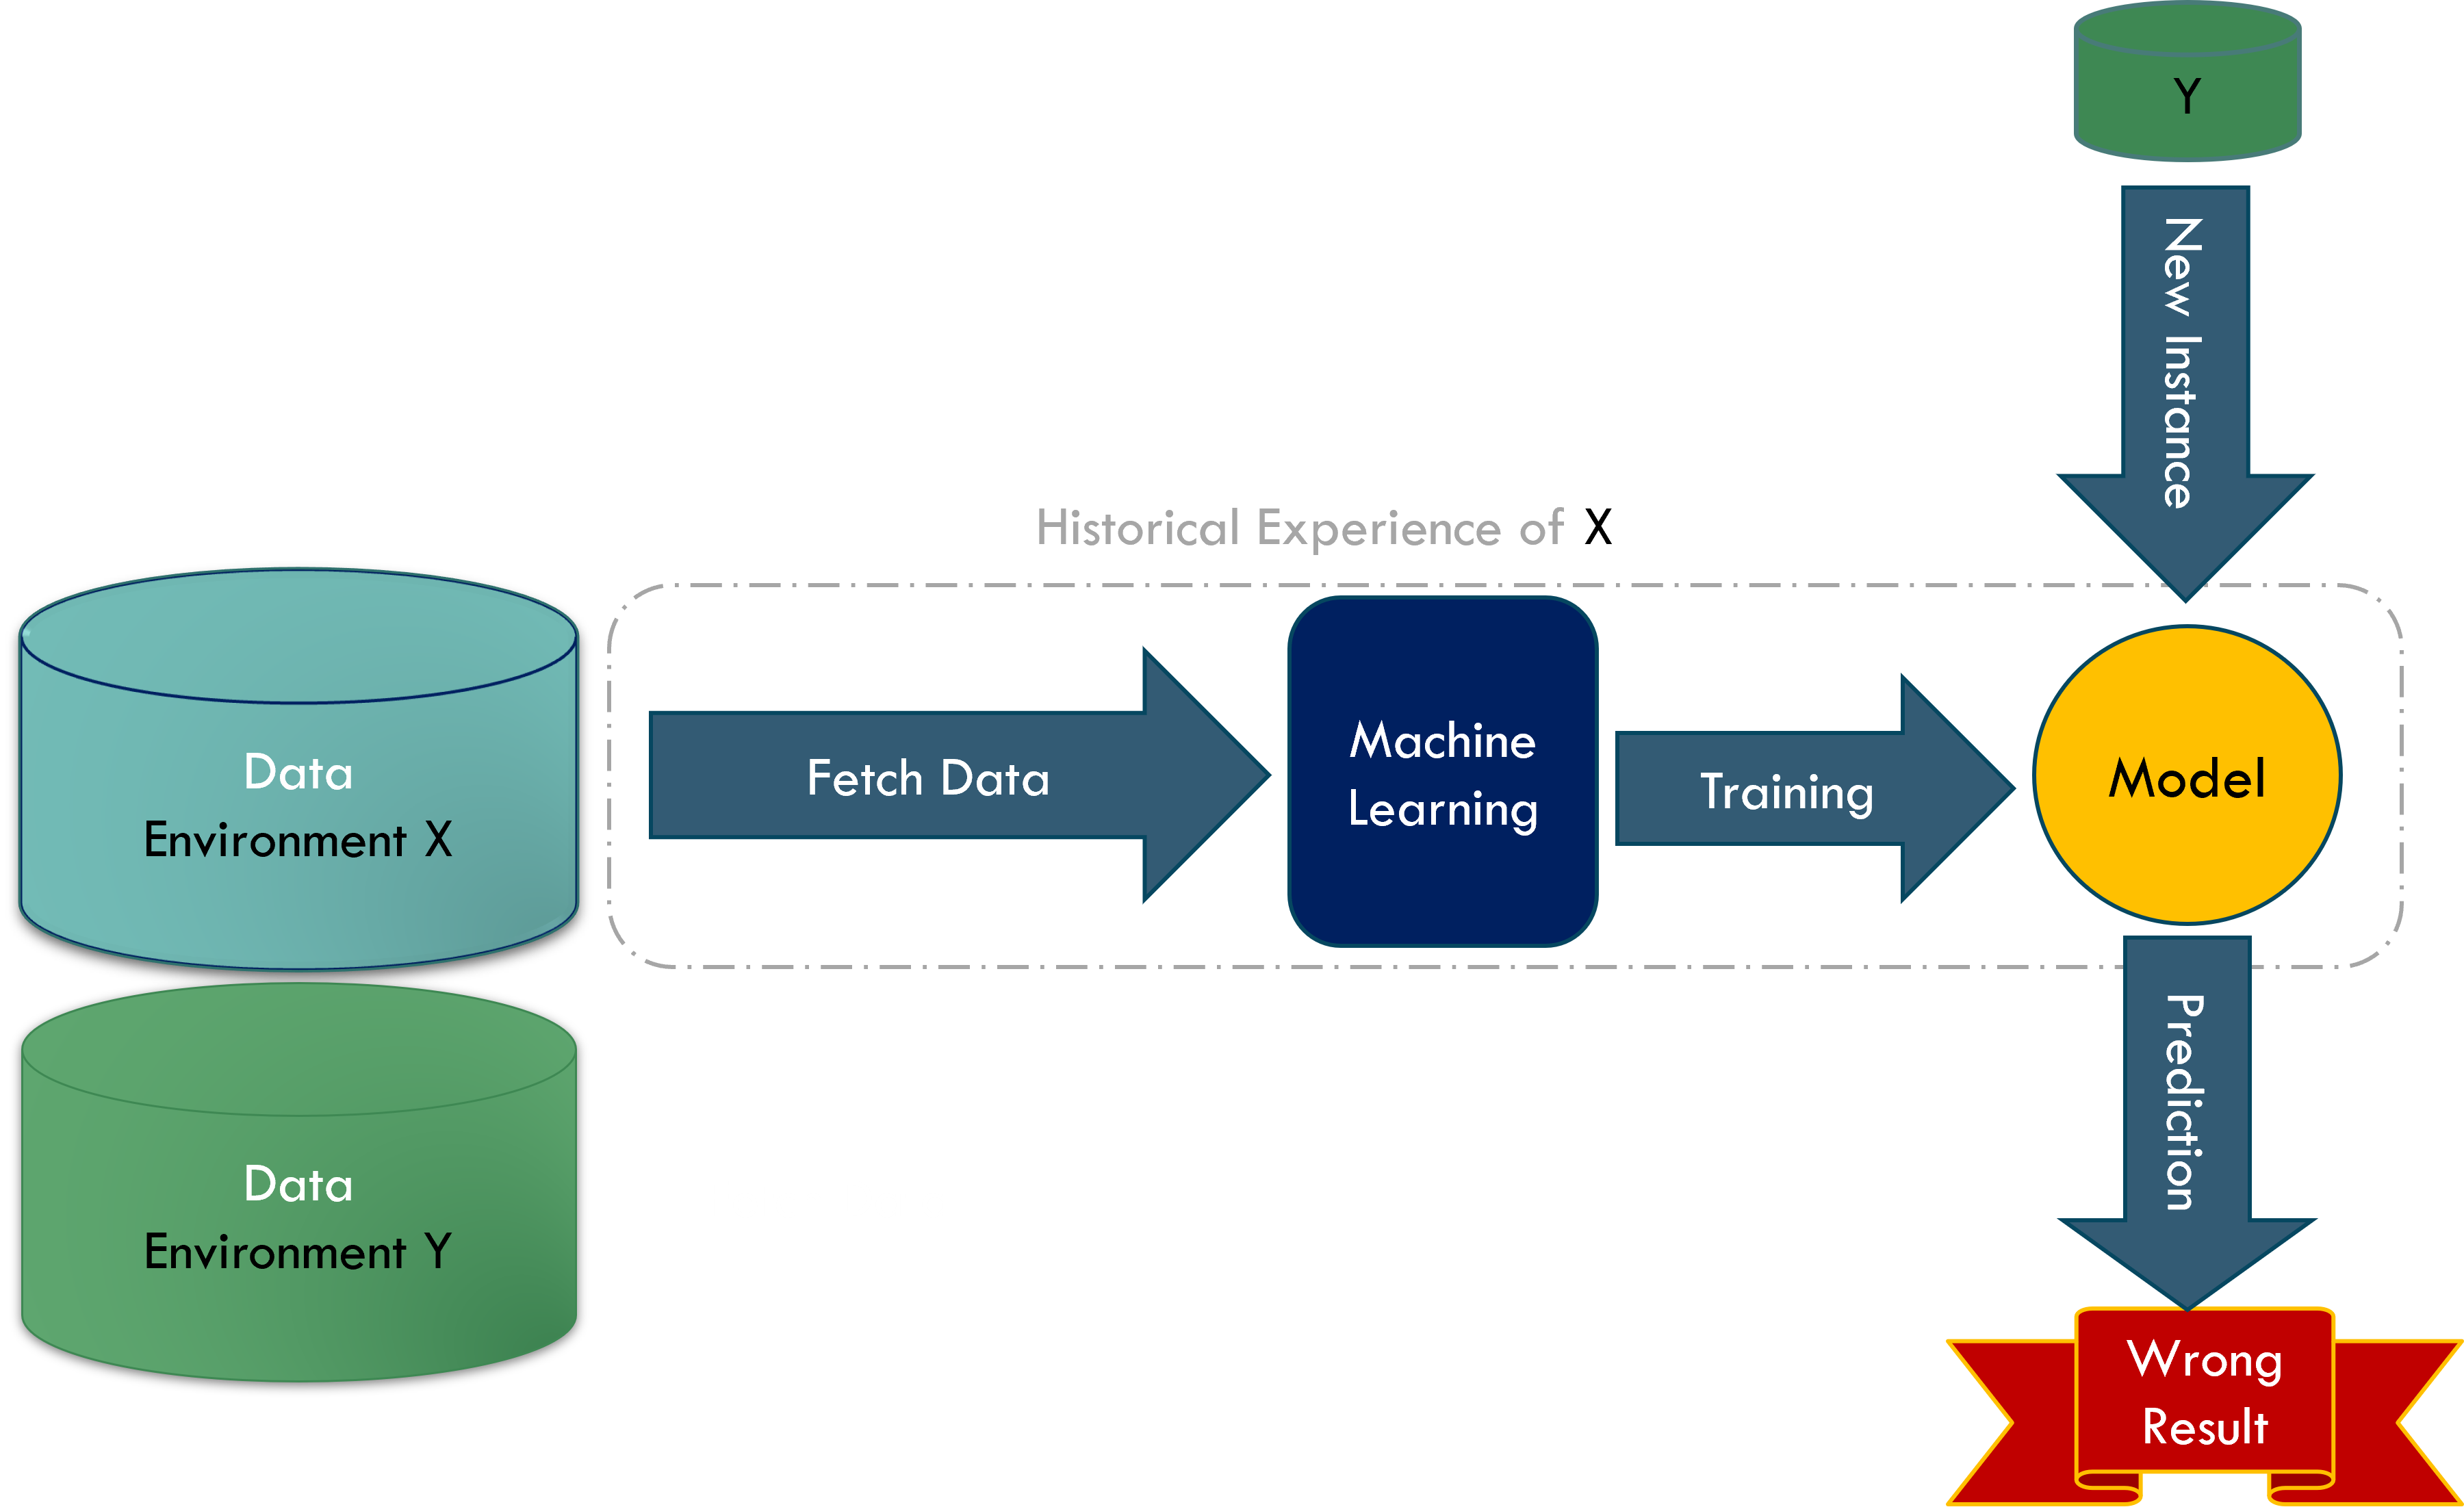
\includegraphics[width=.8\textwidth]{1_introduction/figures/PNG/wrong_machine_flow_1.png}\\
    (a) \\
    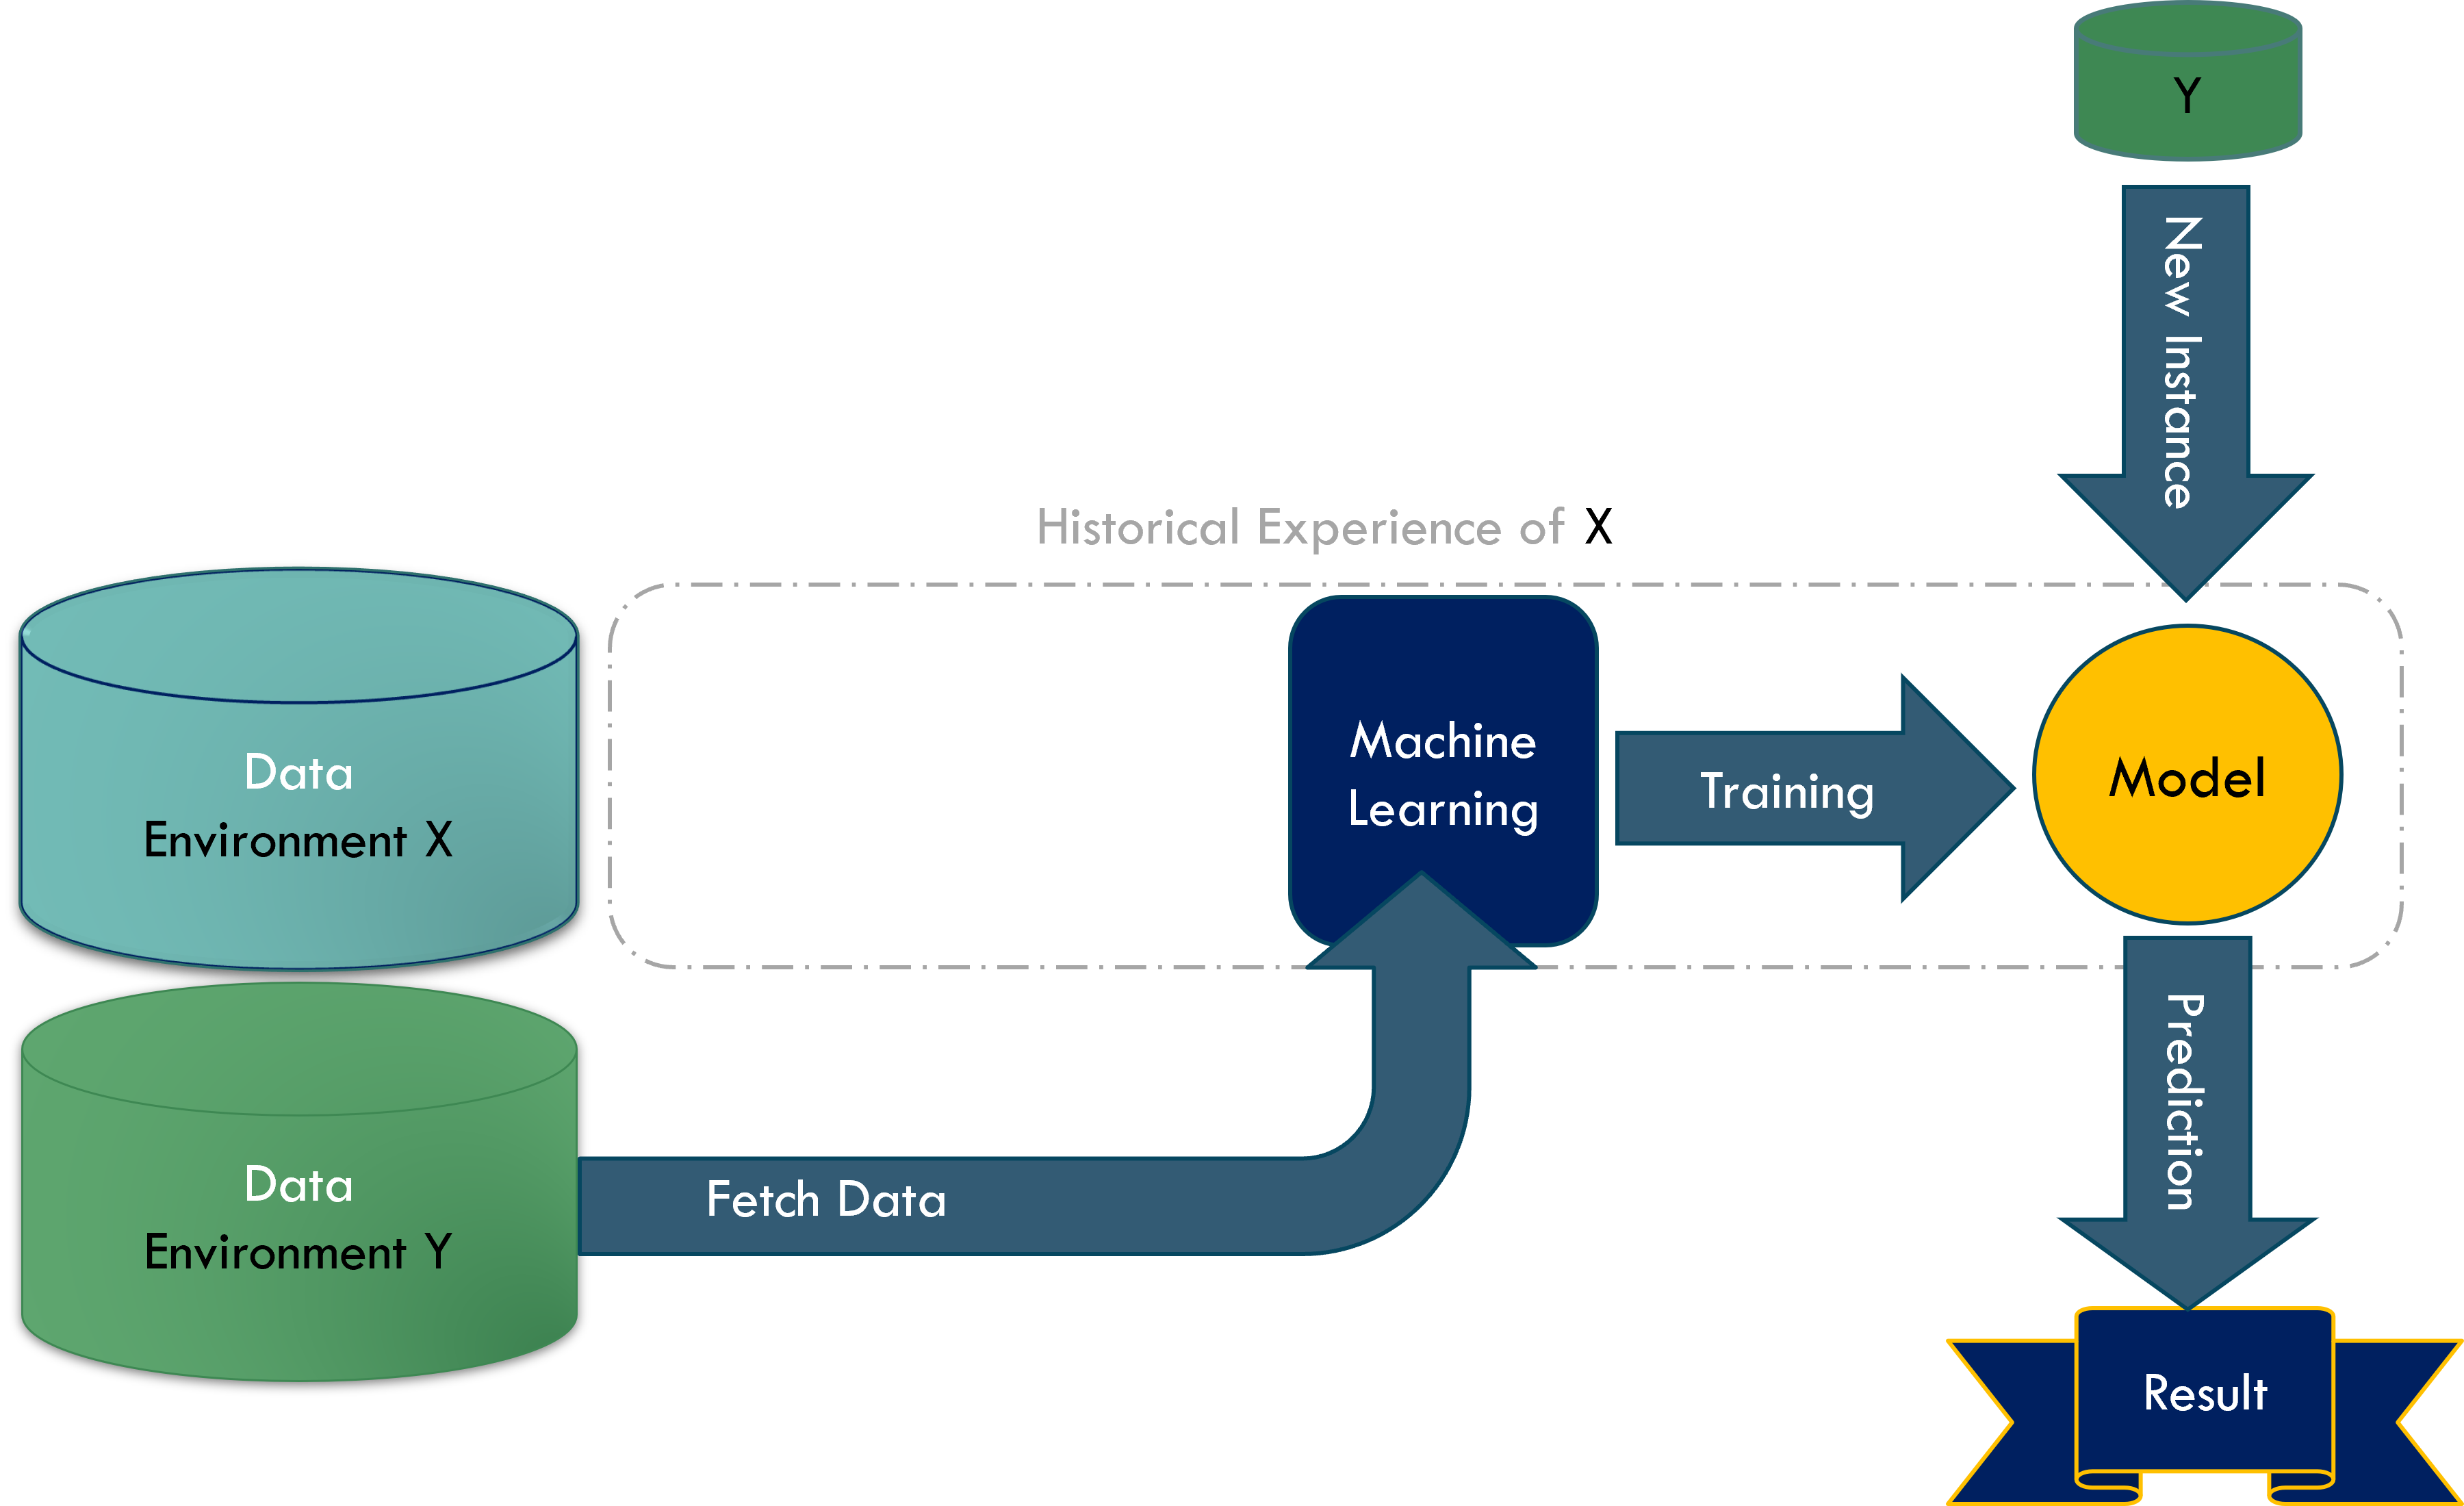
\includegraphics[width=.8\textwidth]{1_introduction/figures/PNG/wrong_machine_flow_2.png}\\
    (b)
    \caption{The research methodology of the thesis.}
    \label{fig:machine-new-senario}
\end{figure}



In recent years, the surge in high-speed data streams has posed notable challenges for machine learning models, particularly in the context of streaming data analysis. These data streams, characterized by continuous, dynamic, and high-volume data arrivals, demand adaptive learning algorithms that can effectively cope with their evolving nature \cite{yang2021concept} \cite{dong2019multistream} \cite{shan2018online}. Within these evolving data environments, two paramount challenges have emerged: concept drift, class imbalance, Emerging new class, and heterogenous transfer learning.

Concept drift, a phenomenon defined by the evolving statistical properties of a data generation process over time \cite{pan2009survey} \cite{zhuang2020comprehensive}. introduces a dynamic element to the data, necessitating continuous adaptation of machine learning models. This shift can manifest as changes in underlying concepts, relationships between variables, or alterations in data distribution. Traditional models trained on historical data may suffer diminished accuracy or become inadequate when confronted with new data influenced by concept drift, highlighting the need for effective concept drift detection mechanisms. Addressing concept drift involves the utilization of concept drift detectors, which are methods capable of identifying changes in data stream distributions. These detectors rely on information related to classifier performance or incoming data items to signal the need for model updates, retraining, or even replacing the old model with a new one. The dynamic nature of concept drift necessitates ongoing monitoring and adaptation to maintain the model's efficacy.

Data streams also present challenges related to class imbalance, a condition characterized by uneven distribution among different classes \cite{wang2018systematic} \cite{sun2009classification}. This scenario, especially prevalent in multi-class settings, poses a significant challenge for traditional classifiers. The risk of misclassifying minority class samples due to their limited representation demands specialized techniques to ensure accurate classification without sacrificing the performance of the majority class \cite{charte2015addressing} \cite{charte2015mlsmote} \cite{daniels2017addressing} \cite{liu2018making}. To tackle class imbalance, three primary methods are commonly employed: sampling methods, algorithm adaptation methods, and hybrid methods. Sampling methods involve undersampling the majority class or oversampling the minority class to balance class distribution. Algorithm adaptation methods modify existing algorithms to handle imbalanced data \cite{japkowicz1995novelty} \cite{lopez2012analysis} \cite{zhang2020towards}, while hybrid methods combine data preprocessing with classification techniques, often utilizing ensemble classifiers to effectively mitigate class imbalance and enhance overall classifier performance \cite{chawla2003smoteboost} \cite{wang2010negative} \cite{galar2011review} \cite{cruz2018dynamic}.

Another challenge arising in the context of class imbalance is class overlap, where instances from different classes share the same region in data space \cite{bhowan2012evolving} \cite{galar2011review}. This overlap complicates the task of distinguishing between representative instances of different classes, leading to performance challenges for traditional classifiers referred to as overlapping problems. Recent research introduces class-overlap undersampling methods to address this issue, leveraging local similarities among minority instances to identify potentially overlapping majority instances.

Therefore, both class imbalance and class overlap present significant hurdles in the realm of data stream analysis. Consequently, addressing class imbalance has become crucial in multi-class learning, leading to research efforts focusing on both concept drift and class imbalance challenges. Researchers have explored dynamic ensemble selection (DES) and multi-class oversampling techniques to tackle these issues. Dynamic classifier ensembles offer a unique ability to adapt their composition based on data characteristics, making them valuable in situations with evolving data conditions \cite{cruz2018dynamic}. Researchers focus on the overproduce-and-select approach for classifier ensemble selection methods. The objective of classifier ensemble selection is to choose an optimal subset of classifiers from a larger ensemble. The selection process is guided by various criteria, including individual performance measures, diversity metrics, meta-learning techniques, and performance estimation approaches. This optimization is particularly important in scenarios where a balance between accuracy and computational resource constraints is critical. There are two distinct approaches: static and dynamic selection. Static selection involves assigning classifiers to predefined feature partitions, while dynamic selection adaptively selects classifiers based on their competency \cite{kuncheva2000clustering}. Dynamic selection offers two choices: individual models, known as Dynamic Classifier Selection (DCS), and ensemble models, called Dynamic Ensemble Selection (DES). DCS algorithms enable the selection of the most appropriate classifier for each data point based on its local competencies. In contrast, DES focuses on selecting the optimal classifiers for each instance based on their competence within localized regions \cite{woloszynski2011probabilistic} \cite{lysiak2014optimal} \cite{cruz2017meta} Competency assessment relies on a dynamic selection dataset (DSEL) containing labeled samples. Moreover, innovative techniques like the Randomized Reference Classifier introduce randomness into class supports to enhance adaptability in addressing challenges related to imbalanced data.

Additionally, transfer learning assumes a pivotal role in addressing the intricate challenges posed by dynamic data streams and inherent concept drift. This domain of research focuses on enhancing a model's learning performance within a target domain by harnessing knowledge gleaned from source domains \cite{pan2009survey} \cite{wang2018systematic}.Techniques in transfer learning include reducing domain gaps through instance re-weighting and feature matching, along with strategies to mitigate negative knowledge transfer by down-weighting irrelevant source data.

Lastly, in the study, the focus extends to the specific scenario of Streams with Emerging New Classes (SENC). This refers to situations where new classes, not present during the initial training of a learning model, emerge in the data stream. Traditional learning approaches, designed for fixed or predefined class distributions, face challenges in effectively recognizing and adapting to these novel classes in real-time. The need for adaptive learning mechanisms that can handle the emergence of new classes underscores the complexity of real-world data stream scenarios.
     

In this chapter, the challages for this research 
that naturally arise is discussed in  Section \ref{sec:1_introduction_challange}. After this, the the motivation, scope and solution methodology are presented in Section \ref{sec:1_introduction_motivation} . After this, the objectives and
esearch questions are presented in Sections \ref{sec:1_introduction_objectives} and \ref{sec:1_introduction_questions}, respectively. Next, the
research contribution is summarised in Section \ref{sec:1_3_automl_and_tf}. Next the research publication is presented in Section \ref{sec:1_introduction_publication}. Finally,
the research methodology and the outline of this thesis are presented in Sections \ref{sec:1_introduction_methodology} and
\ref{sec:1_introduction_organizations}, respectively.
\section{Challenges}
\label{sec:1_introduction_challange}
Within the swiftly evolving realm of machine learning, the proliferation of high-speed data streams presents a significant hurdle — the proficient management of non-stationary data environments. This challenge is marked by dynamic fluctuations in statistical attributes, fundamental concepts, and data distributions over time. The crux of the issue emerges as models, initially trained on historical data, experience a decline in accuracy when confronted with new data influenced by concept drift. This includes scenarios such as:
\begin{itemize}
    \setlength{\itemsep}{0pt}
    \setlength{\parskip}{0pt}
    \item Multi-class imbalanced data streams
    \item Overlapping classes
    \item Emergence of new classes
    \item Heterogeneous transfer learning
\end{itemize}
However, addressing these challenges yields substantial benefits. By effectively managing non-stationary data environments, organizations can enhance the adaptability and resilience of their machine learning systems. This enables more robust decision-making processes, improved predictive capabilities, and heightened performance across diverse contexts. Moreover, it fosters innovation and agility, empowering organizations to stay ahead in dynamic markets and evolving scenarios.

\section{Thesis Motivations}
\label{sec:1_introduction_motivation}

The swift progress in machine learning, particularly in real-time data streams, introduces new challenges that demand innovative solutions. This thesis seeks to address the limitations of traditional models in dynamic, non-stationary data environments. The motivations behind this research are as follows:
\begin{itemize}
    \setlength{\itemsep}{0pt}
    \setlength{\parskip}{0pt}
    \item \textbf{Adapting to Emerging Classes in Real-Time:} New classes within data streams can cause a decline in accuracy. The goal is to develop adaptive mechanisms that quickly incorporate new classes, maintaining system relevance.
    \item \textbf{Proactive Management of Concept Drift:} Concept drift degrades model performance as data properties change. This research focuses on strategies to detect and manage concept drift to maintain model accuracy.
    \item \textbf{Dynamic Optimization of Classifier Ensembles:} To handle emerging classes and shifting distributions, we aim to develop techniques for real-time optimization of classifier ensembles.
    \item \textbf{Addressing Multi-Class Imbalance:} Imbalanced multi-class distributions often lead to biased classification. The thesis aims to create methods that address class imbalances dynamically, ensuring fair classification.
    \item \textbf{Enhancing Transfer Learning in Non-Stationary Environments:} Transfer learning can suffer from negative transfer in non-stationary settings. The research focuses on frameworks that minimize negative transfer and enhance knowledge sharing across diverse domains.
\end{itemize}

\section{Thesis Objectives}
\label{sec:1_introduction_motivation}
The thesis objectives for our research stems from the imperative need to address the following key motivations:
\begin{itemize}
    \item \textbf{Objective 1}. Thandling Imbalanced Multiclass Drifted Data and overlapping classes streams.
    \item \textbf{Objective 2}. addressing Emerging New Classes in Incremental Streams via Concept Drift and K-means Techniques.
    \item \textbf{Objective 3}. addressing Heterogeneous Transfer Learning Problem in data streams via Concept Drift and Eigenvector Techniques.
\end{itemize}

\section{Thesis Questions}
\label{sec:1_introduction_questions}

\begin{itemize}[nosep]
    \setlength{\itemindent}{-.5in}
       \item $\pmb{Q_1}$. What is the impact of imbalanced stream on the performance of ML models in Nonstationary Environment?
        \item $\pmb{Q_2}$. What is the impact of reducing overlapping classes stream on the performance of ML models in Nonstationary Environment?
        \item $\pmb{Q_3}$.How does the emergence of new classes in data streams affect the stability and performance of ML models?
        \item $\pmb{Q_4}$. how can ML models be adapted to accommodate such changes?
        \item $\pmb{Q_5}$. how to employee concept drift to solve the emerging new classes problem?
        \item $\pmb{Q_6}$. How does the Heterogeneous sources in data streams affect the stability and performance of Transfer Learning Technique?
        \item $\pmb{Q_7}$. What approaches or techniques can be employed in heterogeneous transfer learning to facilitate knowledge transfer across diverse sources and domains?
    \end{itemize}
    
\section{Contributions}
\label{sec:1_introduction_contribution}
Our research endeavors to create advanced frameworks designed for effectively managing non-stationary data streams while prioritizing high accuracy and minimizing computational complexity. The key contributions of our work can be summarized as follows:
\begin{itemize}
    \item \textbf{Incorporation of Concept Drift Detection and Ensemble Classifier:} Our primary innovation involves incorporating a concept drift detection method alongside an ensemble classifier. This integration enables real-time adaptation and refinement of our proposed framework in response to transfer learning in non-stationary environments. This methodology ensures the continuous evolution of our classification model in alignment with the changing data landscape.
    \item \textbf{Dynamic Classifier Ensemble Framework for Emergence Class Problem:} We introduce a classification framework that harnesses dynamic classifier ensemble techniques to address the emergence class problem. This framework enhances the performance of classification algorithms when dealing with non-stationary data streams featuring emerging new classes. By dynamically adjusting the ensemble based on data characteristics, our framework improves the accuracy and effectiveness of classification models, effectively tackling challenges associated with emerging new classes.
    \item \textbf{Introduction of Precise Weighting Method for Local Classifiers of the transfer learning framework:} A significant advancement in our research is the introduction of a precise weighting method to assess the significance of each local classifier within the ultimate classifier. This method enhances the accuracy of the overall classifier by providing a nuanced evaluation of individual classifier contributions.
    \item \textbf{Development of Innovative Framework using Eigenvector Technique for addressing heterogenous transfer learning problem:} A significant stride in our research involves the creation of an innovative framework, harnessing the power of the eigenvector technique. This framework is specifically designed to tackle the challenges posed by heterogeneous transfer learning problems. By leveraging the eigenvector technique, our framework enables the seamless transfer of knowledge from diverse source domains to the target domain, thereby enhancing adaptability and overall performance.
    \item \textbf{Dynamic Adjustment Method to Multi-class Imbalanced Data:} Our classification framework introduces a dynamic adjustment method tailored for multi-class imbalanced data scenarios. It seamlessly incorporates concept drift detection mechanisms and optimizes classifier ensemble selections, aiming to significantly improve classification accuracy in the context of multi-class imbalanced non-stationary streams.
    \item \textbf{Adaptive Method for Class Imbalance:} Additionally, we propose an adaptive method for addressing the class imbalance issue. This method considers data distributions and historical instances of class imbalance, especially in cases where class overlap occurs within multi-class and drifted data streams. The adaptive approach improves classification performance by selecting the most suitable oversampling method based on the unique characteristics of the data stream.
\end{itemize}


\section{Publications}
\label{sec:1_introduction_publication}
\begin{table}[h]
 \centering
 \resizebox{\textwidth}{!}{
\renewcommand{\arraystretch}{1.1}
\begin{tabular}{l}
\hline
\textbf{Title:} Dynamic Classification Ensembles for Handling Imbalanced Multiclass Drifted Data Streams.\\
\textbf{Authors:} Madkour, Ahmed H.,Hatem M. Abdelkader, and Amgad M. Mohammed\\
 \textbf{Journal:} Information systems (Impact Factor $=$ 8,1 $\rightarrow$ Q1).\\
 \textbf{Status:} Published. \\ \hline

 \textbf{Title:} Historical Isolated Forest for detecting and adaptation concept drifts in non-stationary data streaming.\\
 \textbf{Authors:} Madkour, Ahmed H.,Hatem M. Abdelkader, and Amgad M. Mohammed.\\
 \textbf{Journal:}  IJCI. International Journal of Computers and Information, 10.2 2023. \\ \textbf{Status:} Published.\\ \hline

\textbf{Title:} Addressing Emerging New Classes in Incremental Streams via Concept Drift Techniques.\\
 \textbf{Authors:} Ahmed H., Madkour, Enrique Onieva, Hatem M. Abdelkader, and Amgad M. Mohammed.\\
 \textbf{Journal:} Information Systems (Impact Factor $=$ 3,0 $\rightarrow$ Q1).\\
 \textbf{Status:} Under review. \\ \hline
 


 
\textbf{Title:} Addressing Heterogeneous Transfer Learning Problem in data streams via Concept Drift.\\
\textbf{Authors:} Ahmed H., Madkour, Enrique Onieva, Hatem M. Abdelkader, and Amgad M. Mohammed.\\
 \textbf{Journal:} Evolving Systems (Impact Factor $=$ 2.8 $\rightarrow$ Q2).\\
 \textbf{Status:} Under review. \\ \hline
 
 
\end{tabular}
 }
 \caption{Publications in journals and conferences conducted during this thesis.}
\label{ch1.publication.list}
\end{table}
During the research activities of this thesis, several international peer-reviewed
journal articles were published to disseminate the obtained results. The publications can be found in Table \ref{ch1.publication.list}. 

\section{Thesis Plan}
\label{sec:1_introduction_methodology}
\begin{figure}[!ht]
    \centering
    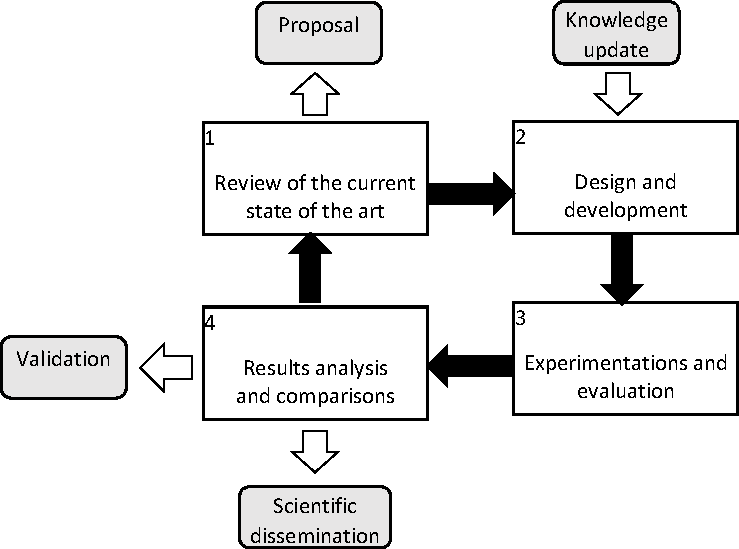
\includegraphics[width=.8\textwidth]{1_introduction/figures/fig_research-methodo.pdf}
    \caption{The Research Plan of Thesis.}
    \label{ch1:research-emthodo}
\end{figure}

The research in this thesis is progressing rapidly due to technological advancements and continuous contributions in machine learning (ML). An iterative research methodology was followed, where each cycle builds upon the knowledge gained in the previous phase, leading to increasingly effective and original solutions as shown in Fig. \ref{ch1:research-emthodo}. The phases of this research methodology are as follows:

\begin{enumerate}
    \setlength{\itemsep}{0pt}
    \setlength{\parskip}{0pt}
    \item \textbf{Review of the current state-of-the-art:} Investigate existing research to identify challenges and inform the design of a solution.
    \item \textbf{Design and development:} Design a novel solution using updated knowledge to address the identified challenges.
    \item \textbf{Experimentation and evaluation:} Test the solution through experimentation, using established criteria for comparison.
    \item \textbf{Results analysis and comparison:} Analyze and compare results with state-of-the-art to determine the effectiveness of the solution, and disseminate the findings.
\end{enumerate}



\section{Structure of the Dissertation}
\label{sec:1_introduction_organizations}
The structure of the remainder of this thesis dissertation is outlined below.
\begin{itemize}	
	\item \textbf{Chapter~\ref{cha:2_background}} reviews background about concept drift, concept drift types, concept drift components, adapting types.  
	
	\item \textbf{Chapter~\ref{cha:3_State-of-the-art}} reviews state-of-the-art  concept drift, classifier ensemble selection, imbalanced data streams, Streams with Emerging New Classes (SENC), and transfer learning.  
	
	\item \textbf{Chapter~\ref{chapter:4_Imbalanced_Multiclass}
	} presents our first proposal to build an effective proposed approch for  handling Imbalanced Multi-class Drifted Data streams.
	
	\item \textbf{Chapter~\ref{chapter:5_emerging}} provides our second proposal to adressing emerging new classes in incremental streams via concept drift techniques. 
	
	\item \textbf{Chapter~\ref{chapter:6_transfer_learning}} presents our third proposal to addressing heterogeneous transfer learning problem  in incremental streams via concept drift techniques.
	
	\item \textbf{Chapter~\ref{chapter:7_Conclusions}} revisits the main goal and specific objectives posted earlier. In this chapter, we summarise the main contributions of this thesis and outline possible future research.


\end{itemize}

% background
% this file is called up by thesis.tex
% content in this file will be fed into the main document


\chapter{Background}\label{cha:2_background}

Amidst the surge of vast streaming data, governments and businesses find themselves in an urgent need for sophisticated data analysis and machine learning analytics approaches. These tools are indispensable for anticipating future trends and making well-informed decisions. However, the perpetual emergence of new goods, markets, and consumer behaviors introduces a formidable challenge known as concept drift \cite{widmer1996learning}. This phenomenon involves the variation of statistical parameters of the target variable over time in unexpected ways, posing a substantial obstacle to accurate forecasting and optimal decision-making. The patterns derived from historical data may become obsolete when applied to new and evolving datasets.
The impact of concept drift extends across data-driven information systems, including decision support and early warning systems, diminishing their overall effectiveness. In the dynamic realm of big data, where data types and distributions are inherently unpredictable, the challenge of concept drift becomes even more pronounced. In response to this challenge, the field introduces a new subject: adaptive data-driven prediction/decision systems.

\section{Concept Drift Sources}
\vspace{-3mm}
\begin{figure}[H]
    \centering
    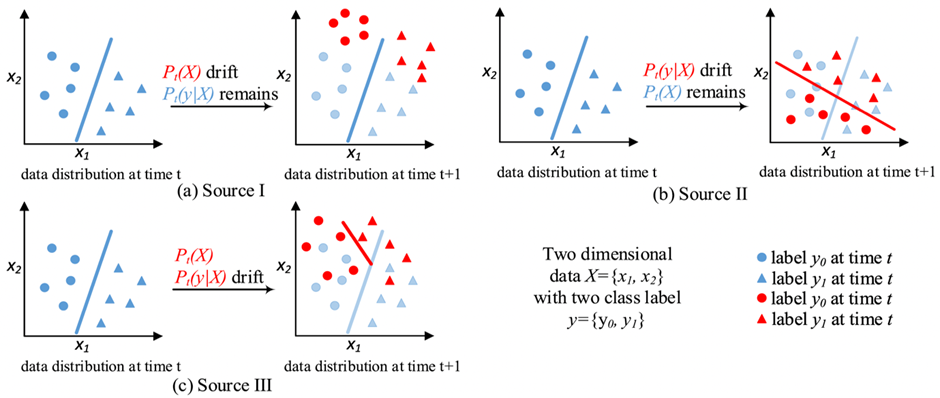
\includegraphics[width=1.0\textwidth]{2_Background/figures/concept_drift_sources.png}
    \caption{Sources of Concept Drift \cite{8496795}. \\ \textcolor{gray}{\fontsize{10}{0}\selectfont DOI: 10.1109/TKDE.2018.2876857}}
    \label{fig:concept-drift-sources}
\end{figure}
\vspace{-6mm}
\label{sec:background_concept_drift_sources}
Concept drift, as illustrated in Fig. \ref{fig:concept-drift-sources}, occurs in three distinct scenarios. First, (a) depicts a shift in data distribution, indicating changes in the underlying patterns and characteristics of incoming data, challenging the model's ability to adapt to new trends \cite{lu2016concept, gama2014survey, losing2016knn, storkey2008training}. Second, (b) shows a change in function output, requiring adjustments in the class delimiter's position as the relationship between input features and output classes evolves. Lastly, (c) represents a dual shift in both data distribution and function output, a more complex form of concept drift that requires the model to adapt to simultaneous changes in patterns and output relationships. Effectively managing these shifts is essential for maintaining predictive accuracy and decision-making in dynamic environments, highlighting the importance of adaptive strategies in machine learning models.



\section{Concept Drift Types}
\label{sec:background_concept_drift_types}
Concept drift is categorized into four types, as shown in Fig. \ref{fig:concept-drift-types}. Types 1-3 focus on minimizing accuracy loss and maximizing recovery during concept transformation. Type 4, however, emphasizes leveraging historical concepts to identify the best-matched concept during new concept emergence. The term "intermediate concept," introduced by \cite{losing2016knn}, refers to transitional phases between concepts. \cite{liu2018making} further notes that concept drift can extend over time, with intermediate concepts representing a blend of starting and ending concepts in incremental drift or one of these in gradual drift. Understanding these intermediate concepts is key to grasping the dynamics of concept drift during transitions.
\vspace{-3mm}
\begin{figure}[H]
    \centering
    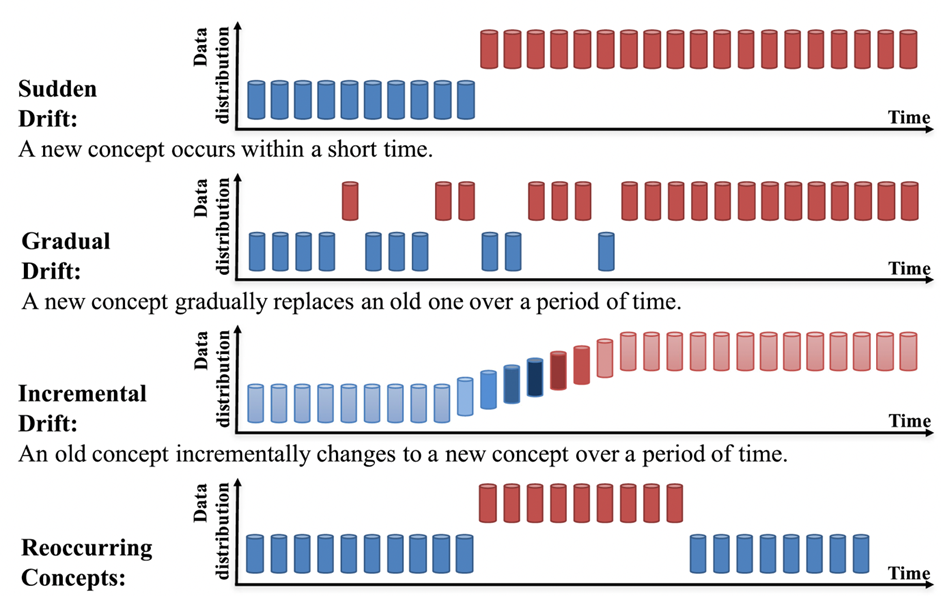
\includegraphics[width=0.8\textwidth]{2_Background/figures/concept_drift_types.png}
    \caption{Types of Concept Drift \cite{8496795}. \\ \textcolor{gray}{\fontsize{10}{0}\selectfont DOI: 10.1109/TKDE.2018.2876857}}
    \label{fig:concept-drift-types}
\end{figure}
\vspace{-6mm}


\section{Concept Drift Components}
\label{sec:background_concept_drift_components}
Conventional machine learning primarily involves prediction and training/learning. However, learning under the concept drift paradigm introduces three additional critical steps as show in Fig. \ref{fig:concept-drift-components}: concept drift detection, drift understanding, and drift adaptation. Concept drift detection involves identifying changed points or change time periods to define and predict drift. Drift understanding delves into crucial aspects such as when the drift starts, how long it lasts, and where it occurs, providing indispensable insights for the subsequent adaptation step.  
The adaptation step, also referred to as the reaction step, plays a pivotal role in updating current learning models in response to concept drift. Three main approaches address various types of drift: Simple Retraining, Ensemble Retraining, and Model Adjusting. Drift detection employs various tools and algorithms, comparing old and fresh data chunks with statistical models based on data distribution. Techniques vary, with some utilizing a constant chunk length and others employing a variable length.
Drift understanding is essential for making well-informed decisions during the adaptation step. This involves calculating the necessary modifications in the trained model to adapt to new changes as shown in Fig. \ref{fig:concept-drift-understanding}. The severity region determines whether to generate a completely new model or make minimal adjustments to the existing one.

 
\begin{figure}[!ht]
    \centering
    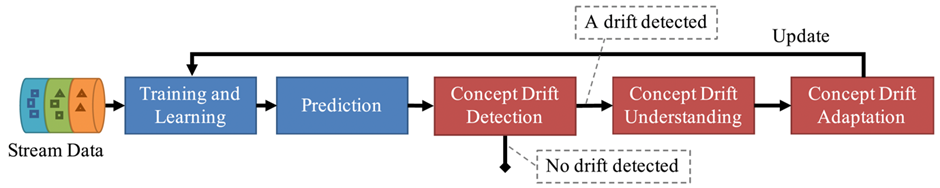
\includegraphics[width=.9\textwidth]{2_Background/figures/concept_drift_components.png}
    \caption{Main components of concept drift. \\ \textcolor{gray}{\fontsize{10}{0}\selectfont DOI: 10.1109/TKDE.2018.2876857}}

    \label{fig:concept-drift-components}
\end{figure}


%==============================[detection subsection]===============
\subsection{Concept Drift Detection}
Drift detection involves techniques and mechanisms to characterize and quantify concept drift by identifying change points or intervals \cite{liu2018making}. The general framework for drift detection consists of four stages:
\begin{itemize}
    \item \textbf{Stage 1 (Data Retrieval):} This stage focuses on retrieving data chunks from data streams. Given that a single data instance lacks sufficient information to infer the overall distribution \cite{lu2016concept}, organizing data chunks meaningfully is crucial for effective data stream analysis \cite{ramirez2017survey}.
    \item \textbf{Stage 2 (Data Modeling):} This optional stage abstracts the retrieved data, extracting key features that contain sensitive information impacting a system in case of drift. This stage may involve dimensionality reduction or sample size reduction to meet storage and online speed requirements \cite{liu2018making}.
    \item \textbf{Stage 3 (Test Statistics Calculation):} This stage involves measuring dissimilarity or estimating distance to quantify drift severity and generate test statistics for hypothesis testing. Defining an accurate and robust dissimilarity measurement remains a challenging aspect of concept drift detection. Test statistics can also be used for clustering evaluation \cite{silva2013data} and to determine dissimilarity between sample sets \cite{dries2009adaptive}.
    \item \textbf{Stage 4 (Hypothesis Test):} This stage employs a specific hypothesis test to assess the statistical significance of the change observed in Stage 3, such as the p-value. These tests determine drift detection accuracy by establishing statistical bounds for the test statistics from Stage 3. Without Stage 4, the acquired test statistics are meaningless for drift detection, as they cannot establish the drift confidence interval. Commonly used hypothesis tests include estimating the distribution of test statistics \cite{alippi2008just} \cite{gama2004learning}, bootstrapping \cite{bu2016pdf} \cite{venkatasubramanianinformation}, the permutation test \cite{lu2016concept}, and Hoeffding's inequality-based bound identification \cite{frias2014online}.
\end{itemize}

It is crucial to note that without Stage 1, the concept drift detection problem can be regarded as a two-sample test problem, examining whether the populations of two given sample sets are from the same distribution \cite{dries2009adaptive}. In other words, any multivariate two-sample test can be adopted in Stages 2-4 for detecting concept drift \cite{dries2009adaptive}. However, in cases where distribution drift may not be included in the target features, the selection of the target feature becomes critical for the overall performance of a learning system and poses a significant challenge in concept drift detection \cite{yamada2013change}.

%==============================[detection Understanding]===============
\subsection{Understanding Phase}
The extent of concept drift severity serves as a valuable criterion for selecting appropriate drift adaptation strategies. As shown in Fig. \ref{fig:concept-drift-understanding}, in a classification task where the drift's severity is minimal, resulting in only a marginal shift in the decision boundary within the new concept, adjusting the current learner through incremental learning proves sufficient. Conversely, when confronted with high severity in concept drift, wherein the decision boundary undergoes substantial changes, it might be more effective to discard the old learner and opt for retraining a new one rather than incrementally updating the existing learner. It's noteworthy to mention that despite some researchers highlighting the capability to articulate and quantify the severity of detected drift, this information is not yet widely integrated into drift adaptation practices.
The adaptation step offers three distinct ways to adapt the model. Simple Retraining involves training a new model using the most recent data, replacing the old model. Model Ensemble, the second approach, entails keeping and reusing existing models, which proves efficient when dealing with repeated instances of concept drift. The third approach, Model Adjusting, constructs a model that adapts flexibly from changed data, allowing partial updates when the original data distribution undergoes significant changes.

\begin{figure}[!ht]
    \centering
    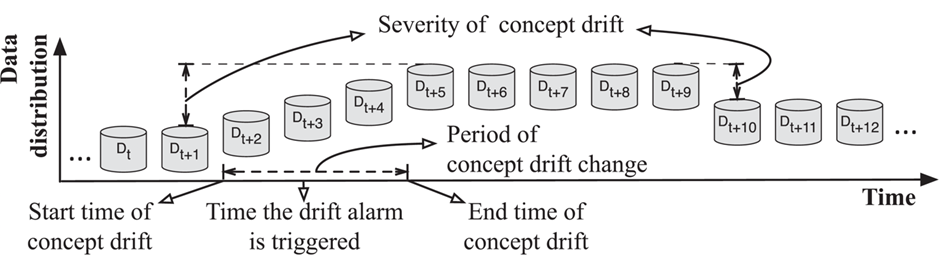
\includegraphics[width=.9\textwidth]{2_Background/figures/concept_drift_understanding.png}
    \caption{Understanding phase of concept drift. \\ \textcolor{gray}{\fontsize{10}{0}\selectfont DOI: 10.1109/TKDE.2018.2876857}}
    \label{fig:concept-drift-understanding}
\end{figure}

%==============================[Adaptation Adaptation]===============
\subsection{Adaptation Phase}
This section delves into strategies for updating existing learning models in response to drift, referred to as drift adaptation or reaction. The three primary categories of drift adaptation methods are simple retraining, ensemble retraining, and model adjusting, each tailored to address specific types of drift.

\begin{enumerate}[label=\Alph*.]
    \item \textbf{Simple Retraining} \\
    One way to respond to concept drift is by retraining a new model with the latest data, replacing the outdated model as shown in Fig.\ref{fig:concept-drift-adaptation}. This approach requires an explicit concept drift detector to determine when to retrain the current model. A window strategy is commonly used, preserving recent data for retraining and/or utilizing old data for distribution change tests. An example of this strategy is Paired Learners \cite{bach2008paired}, which employs two learners: the stable learner and the reactive learner. If the stable learner consistently misclassifies instances correctly classified by the reactive learner, indicating a new concept, the stable learner is replaced with the reactive learner. This method is straightforward, easy to implement, and adaptable at any point in the data stream.
    However, a trade-off arises when adopting a window-based strategy in determining an appropriate window size. A small window better reflects the latest data distribution, while a large window provides more data for training a new model. To address this challenge, the ADWIN algorithm \cite{bifet2007learning} dynamically adjusts sub window sizes based on the rate of change between two sub-windows, eliminating the need for users to predefine window sizes.
    Beyond direct model retraining, researchers have explored integrating the drift detection process with the retraining process for specific machine learning algorithms. DELM \cite{xu2017dynamic}, for instance, extends the traditional ELM algorithm, adapting to concept drift by dynamically adjusting the number of hidden layer nodes in response to increasing classification error rates, indicating a potential concept drift.
    Similarly, FP-ELM \cite{liu2016fp} introduces a forgetting parameter to the ELM model to adapt to drift conditions. A parallel version of the ELM-based method \cite{han2015efficient} has been developed for high-speed classification tasks under concept drift. OS-ELM \cite{soares2016adaptive}, an online learning ensemble of repressor models, integrates ELM using an ordered aggregation (OA) technique to address the challenge of defining the optimal ensemble size.
    In the realm of instance-based lazy learners for handling concept drift, the Just-in-Time adaptive classifier \cite{alippi2008just}  follows the "detect and update model" strategy, extending the traditional CUSUM test \cite{manly2000cumulative} to a pdf-free form for drift detection. When a concept drift is identified, old instances (beyond the last T samples) are removed from the case base. Advancements include extending this algorithm to handle recurrent concepts by considering and comparing the current concept to previously stored concepts \cite{silva2013data} \cite{alippi2008just}. NEFCS \cite{lu2016concept}, another KNN-based adaptive model, employs a competence model-based drift detection algorithm \cite{lu2016concept} to locate drift instances in the case base and distinguish them from noise instances. The redundancy removal algorithm, Stepwise Redundancy Removal (SRR), is developed to eliminate redundant instances uniformly, ensuring that the reduced case base retains sufficient information for future drift detection.
    

\begin{figure}[!ht]
    \centering
    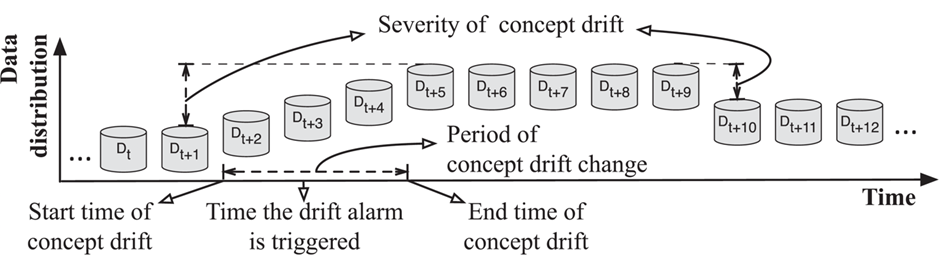
\includegraphics[width=.9\textwidth]{2_Background/figures/concept_drift_understanding.png}
    \caption{Approach for retraining a new model. \\ \textcolor{gray}{\fontsize{10}{0}\selectfont DOI: 10.1109/TKDE.2018.2876857}}
    \label{fig:concept-drift-adaptation}
\end{figure}





\item \textbf{Model Ensemble for Recurring Drift} \\
In recurring concept drift scenarios, preserving and reusing old models can be more efficient than retraining new ones for each recurrence, forming the basis for employing ensemble methods \cite{sun2018concept}. These methods, a focus in stream data mining research, consist of base classifiers with varied types or parameters. Their outputs, determined by specific voting rules, collectively predict new data. Various adaptive ensemble methods, extending classical ones or introducing adaptive voting rules, address the challenges of concept drift as shown in Fig. \ref{fig:concept-drift-ensemble}.
Classical ensemble methods like Bagging, Boosting, and Random Forests have been adapted for streaming data with concept drift. For instance, online Bagging \cite{oza2001experimental} uses each instance once, simulating batch mode bagging. Leveraging Bagging \cite{bifet2009new} employs ADWIN drift detection to replace the existing classifier with the worst performance when concept drift is detected.
 Adaptive boosting \cite{chu2004fast}, monitoring prediction accuracy through a hypothesis test, addresses concept drift, assuming classification errors on non-drifting data follow a Gaussian distribution. The Adaptive Random Forest (ARF) algorithm \cite{gomes2017adaptive} extends the random forest tree algorithm, incorporating concept drift detection (e.g., ADWIN) to decide when to replace an obsolete tree. A similar approach is seen in \cite{li2015learning}, using Beyond classical methods, novel ensemble methods with innovative voting techniques tackle concept drift. Dynamic Weighted Majority (DWM) \cite{kolter2007dynamic} adapts to drifts through weighted voting rules, managing base classifiers based on individual and global ensemble performance. Learn++NSE \cite{elwell2011incremental} addresses frequent classifier additions by weighting them based on prediction error rates.
 Specific types of concept drift are considered in specialized ensemble methods. Accuracy Update Ensemble (AUE2) \cite{brzezinski2013reacting} equally addresses sudden and gradual drift, using a batch mode weighted voting ensemble method. Optimal Weights Adjustment (OWA) \cite{zhang2008categorizing} achieves a similar goal with weighted instances and classifiers. Special cases, like class evolution, are considered in \cite{sun2016online}, while recurring concepts are handled by monitoring concept information \cite{gomes2013mining} \cite{gama2014survey} .Another method \cite{ahmadi2018modeling}, refines the concept pool for recurring concepts.
 
 \begin{figure}[!ht]
    \centering
    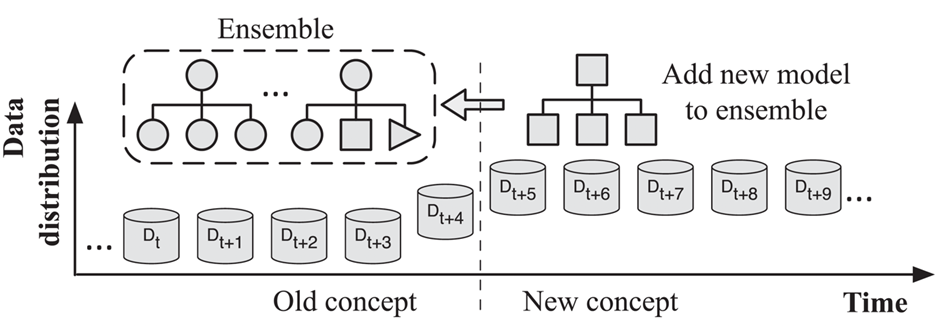
\includegraphics[width=.9\textwidth]{2_Background/figures/ensemble_update.png}
    \caption{Ensemble approach for the adaptation phase. \\ \textcolor{gray}{\fontsize{10}{0}\selectfont DOI: 10.1109/TKDE.2018.2876857}}
    \label{fig:concept-drift-ensemble}
\end{figure}




\item \textbf{Model Ensemble for Recurring Drift} \\
As Shown in Fig. \ref{fig:concept-drift-partial-update}, instead of retraining the entire model, an alternative is to construct a model with adaptive learning capabilities, allowing partial updates in response to changing data distributions \cite{pratama2015evolving}, as in Fig. \ref{fig:concept-drift-partial-update}. This is efficient when concept drift occurs in localized regions. Many techniques in this category use the decision tree algorithm, leveraging its ability to adapt to individual sub-regions.
VFDT \cite{domingos2000mining} is a foundational contribution for high-speed data streams, employing the Hoeffding bound for node splitting. VFDT processes each instance once, doesn't store instances, and has minimal maintenance costs. CVFDT \cite{hulten2001mining}, an extension, addresses concept drift by maintaining a sliding window of the latest data and replacing the original sub-tree with a better-performing alternative.
VFDTc \cite{hulten2001mining} enhances VFDT by handling numerical attributes and adapting to concept drift with node-level detection. Later extensions \cite{yang2012incrementally} \cite{yang2015countering} introduce an adaptive leaf strategy in VFDTc, selecting the best classifier from options like majority voting, Naive Bayes, and Weighted Naive Bayes. Recent studies \cite{rutkowski2012decision}\cite{rutkowski2014new} question VFDT's foundation, the Hoeffding bound, for non-independent variables in information gain. An alternative impurity measure is proposed in a new online decision tree model \cite{rutkowski2014new}, demonstrating its reflection of concept drift and potential use in CVFDT. IADEM-3 \cite{frias2016online} addresses Hoeffding bound concerns by computing the sum of independent random variables for drift detection and pruning.

 \begin{figure}[!ht]
    \centering
    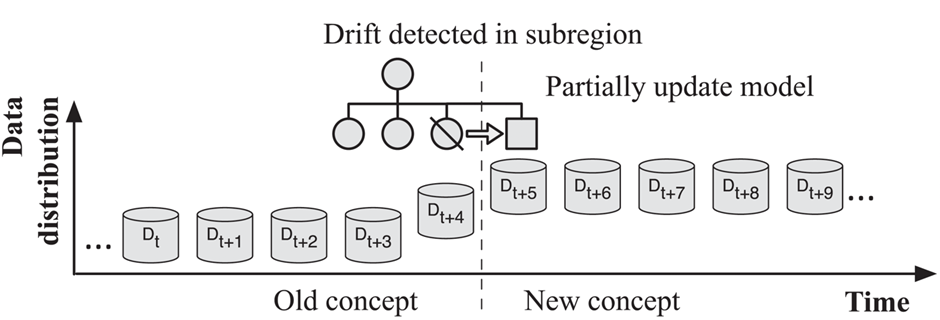
\includegraphics[width=.9\textwidth]{2_Background/figures/partial_update.png}
    \caption{Partial updating approach for the adaptation phase. \\ \textcolor{gray}{\fontsize{10}{0}\selectfont DOI: 10.1109/TKDE.2018.2876857}}
    \label{fig:concept-drift-partial-update}
\end{figure}
\end{enumerate}
% \section{Metrics}
\label{sec:metrics}

The evaluation utilizes several metrics, including recall, precision, F1 score , Balanced Accuracy (BAC), G-mean, and specificity\cite{sasaki2007truth}\cite{kubat1997addressing}\cite{brodersen2010balanced}. These metrics provide a comprehensive view of the classification performance, addressing different aspects such as correctness, balance, and the ability to detect positive and negative cases accurately. The following subsections define each metric used in the evaluation.

\subsection{Recall}
Recall, also known as sensitivity or true positive rate, measures the ability of the classifier to correctly identify positive instances. It is particularly important in scenarios where the detection of positive cases is crucial, such as in medical diagnoses or fraud detection.

\begin{equation}
\text{Recall} = \frac{TP}{TP + FN}
\end{equation}

where $TP$ represents the number of true positives, and $FN$ represents the number of false negatives. A high recall indicates that most of the actual positive cases are correctly classified.

\subsection{Precision}
Precision measures the ability of the classifier to provide relevant positive predictions. It is defined as:

\begin{equation}
\text{Precision} = \frac{TP}{TP + FP}
\end{equation}

where $TP$ represents the number of true positives, and $FP$ represents the number of false positives. Precision is crucial when false positives need to be minimized, for example, in spam detection or quality control systems.

\subsection{F1 Score}
The F1 score is the harmonic mean of precision and recall, and it provides a balanced view of the classifier's performance when both precision and recall are equally important:

\begin{equation}
\text{F1 Score} = 2 \times \frac{\text{Precision} \times \text{Recall}}{\text{Precision} + \text{Recall}}
\end{equation}

A higher F1 score indicates that the model achieves a good trade-off between precision and recall, making it useful in cases where there is an uneven class distribution.

\subsection{Balanced Accuracy (BAC)}
Balanced Accuracy (BAC) is defined as the average of recall for each class, which helps in evaluating the model's ability to correctly classify both positive and negative instances, especially in imbalanced datasets:

\begin{equation}
\text{BAC} = \frac{1}{2} \left( \frac{TP}{TP + FN} + \frac{TN}{TN + FP} \right)
\end{equation}

where $TN$ represents the number of true negatives. BAC is useful when the classes are imbalanced, as it treats both positive and negative classes equally.

\subsection{G-mean}
G-mean is the geometric mean of recall for each class, which measures the balance between classification performance on the positive and negative classes. It is defined as:

\begin{equation}
\text{G-mean} = \sqrt{\frac{TP}{TP + FN} \times \frac{TN}{TN + FP}}
\end{equation}

G-mean is particularly useful in evaluating the performance of models on imbalanced datasets, as it ensures that both classes are predicted with similar accuracy.

\subsection{Specificity}
Specificity, also known as the true negative rate, measures the ability of the classifier to correctly identify negative instances. It is defined as:

\begin{equation}
\text{Specificity} = \frac{TN}{TN + FP}
\end{equation}

where $TN$ represents the number of true negatives, and $FP$ represents the number of false positives. Specificity is crucial in scenarios where false positives need to be minimized, such as in screening tests where a false positive result may lead to unnecessary follow-up procedures.



% state-of-the-art
\chapter{State-of-the-art}
\label{cha:3_State-of-the-art}


In this chapter, we provide a comprehensive review of recent advancements in stream classification, addressing several critical challenges that arise in dynamic data environments. The rapid evolution of data streams introduces complexities such as concept drift, imbalanced multiclass scenarios, class overlap, classifier ensemble selection, emergence of new classes, and the incorporation of transfer learning. This introduction outlines the structure of the chapter and highlights the significance of each topic in advancing stream classification methodologies.
The first section (Setion \ref{sec:3_1_concept_drift}) focuses on concept drift, a phenomenon where the statistical properties of the data change over time. We explore various methodologies developed for real-time detection and adaptation to concept drift in streaming scenarios. This includes a review of techniques that enable systems to identify shifts in data patterns promptly, ensuring sustained classification accuracy. By analyzing the strengths and limitations of these approaches, we highlight the necessity for robust drift detection mechanisms in evolving data streams.
Next, in Section \ref{sec:3_2_ensemble}, we delve into classifier ensemble selection in the context of streaming data. As the characteristics of data streams evolve, selecting the most appropriate ensemble of classifiers becomes crucial. We present algorithms designed to dynamically choose the best-performing classifiers based on the current data distribution. This section emphasizes the importance of adaptive ensemble strategies in enhancing classification performance amidst changing data landscapes.
Section \ref{sec:3_3_imbalanced} addresses the challenges posed by imbalanced multiclass scenarios, particularly in the presence of overlapping classes. We discuss specialized oversampling techniques aimed at countering the effects of class imbalance in streaming data. By providing insights into effective strategies for balancing the representation of minority classes, we lay the groundwork for developing robust frameworks that can maintain performance in imbalanced drifted streams.
As new classes emerge in streaming systems, traditional classifiers often struggle to adapt effectively. In Section \ref{sec:3_4_emergence}, we explore methodologies that specifically focus on the integration of new classes within existing frameworks. This section highlights innovative approaches that enhance the adaptability of stream classification systems, ensuring they remain effective as new data patterns emerge.
In Section \ref{sec:3_5_transfer_learning}, we examine the role of transfer learning in stream classification. This section discusses how transfer learning techniques can leverage knowledge from related tasks to improve classification performance in dynamic environments. We explore current methodologies that facilitate the transfer of information across different domains, particularly in situations where labeled data may be scarce. The insights gained from this discussion will be pivotal for understanding how transfer learning can complement other strategies in our proposed framework.
In Section \ref{sec:3_6_comparsion},To further contextualize our discussion, we conduct a comparative analysis of recent works in the field, focusing on the recent works for each challange. We assess their contributions and identify limitations, illuminating specific gaps in the current research landscape that our work aims to address.
Finally, Section \ref{sec:3_7_remartks} concludes this chapter by identifying key remarks and gaps, which inform the research direction for the subsequent chapters.



%%%%%%%%%%%%%%%%%%%%%%%%%%%%%%%%%%%%%%%%%%%%%%%
%
%   Taxonomies in the Traffic Forecasting Field
%
%%%%%%%%%%%%%%%%%%%%%%%%%%%%%%%%%%%%%%%%%%%%%%%
\section{Concept Drift}
\label{sec:3_1_concept_drift}
Concept drift refers to changes in the underlying data distribution over time, which can reduce the accuracy of previously trained machine learning models \cite{baena2006early, madkour2023historical, tan2022information}. Detecting and responding to concept drift is crucial for maintaining model performance. Several detection methods have been proposed to address this challenge. The Drift Detection Method (DDM) \cite{gama2004learning, bifet2009new} uses a statistical test to identify significant error rate increases, signaling concept drift. The Early Drift Detection Method (EDDM) \cite{gama2004learning, adams2023explainable} extends DDM by considering a moving window of recent data. ADWIN \cite{gama2004learning, adams2023explainable} employs a sliding window to monitor statistical differences and adjusts the window size to adapt to drift patterns. The Kolmogorov-Smirnov windowing method (KSWIN) \cite{adams2023explainable} calculates the Kolmogorov-Smirnov distance to detect drift, while Hoeffding's bounds with moving average test (HDDMA) and its variant HDDMW \cite{gama2004learning, bifet2009new} compute bounds for the true mean to detect distribution changes. Lastly, the Page-Hinkley method \cite{page1954continuous} tracks the cumulative sum of errors, detecting drift when the sum exceeds a threshold. These methods enable machine learning models to adapt to evolving data streams, enhancing model performance and robustness.

%%%%%%%%%%%%%%%%%%%%%%%%%%%%%%%%%%%%%%%%%%%%%%%
%
%   General-purpose Automated Machine Learning
%
%%%%%%%%%%%%%%%%%%%%%%%%%%%%%%%%%%%%%%%%%%%%%%%
\section{Classifier Ensemble Selection}

\label{sec:3_2_ensemble}
This study focuses on the overproduce-and-select approach for classifier ensemble selection methods \cite{cruz2017meta}\cite{kuncheva2000clustering}\cite{jackowski2014improved}. The primary objective of classifier ensemble selection is to identify the optimal subset of classifiers from a larger ensemble, considering various criteria such as performance measures, diversity metrics, meta-learning techniques, and performance estimation approaches. This selection process aims to reduce computational complexity, enhance efficiency, and improve overall ensemble performance, making it highly valuable for real-world applications. By carefully selecting a smaller subset of classifiers, ensemble selection strikes a balance between accuracy and computational resources, adapting to the evolving nature of the data stream. This approach leverages the strengths of different classifiers and adjusts the ensemble composition to handle changing conditions effectively. The goal is to enhance the accuracy, robustness, and overall performance of classification models in dynamic and challenging scenarios. There are two main approaches to the selection process: static and dynamic selection. Static selection assigns classifiers to specific partitions of the feature space, while dynamic selection chooses a classifier specifically for each unknown data sample based on its local competencies. Dynamic Ensemble Selection (DES) is a widely recognized approach that selects the best classifiers for each test instance, considering their competence within the local region of competence. The Randomized Reference Classifier proposed by Woloszynski and Kurzynski \cite{woloszynski2011probabilistic} stands out among various approaches. This classifier introduces randomness through beta distribution, enhancing adaptability and robustness. By considering the stochastic nature of class supports, the Randomized Reference Classifier can potentially improve classification performance in concept drift scenarios. However, it is important to note that employing diversity measures during the classifier selection process, as demonstrated by Lysiak \cite{lysiak2014optimal}, may lead to smaller ensembles but does not necessarily enhance classification accuracy. Overall, the overproduce-and-select approach for classifier ensemble selection methods offers a comprehensive framework for addressing the challenges associated with concept drift. By dynamically adapting the ensemble composition and leveraging the competencies of individual classifiers, this approach aims to improve classification performance, efficiency, and adaptability in dynamic and challenging scenarios.
%%%%%%%%%%%%%%%%%%%%%%%%%%%%%%%%%%%%%%%%%%%%%%%
%
%   Machine Learning for Traffic Forecasting
%
%%%%%%%%%%%%%%%%%%%%%%%%%%%%%%%%%%%%%%%%%%%%%%%
\section{Imbalanced data Streams}
\label{sec:3_3_imbalanced}
In imbalanced data classification, three primary approaches have been identified \cite{yin2022graph}, with our study focusing on the first category that addresses imbalanced data streams through sampling methods, specifically oversampling \cite{ren2023grouping}. This method generates synthetic instances to balance class distributions \cite{nitesh2002smote, han2005borderline, bunkhumpornpat2009safe, maciejewski2011local}. Class imbalance can occur in binary or multi-class scenarios, and our research specifically focuses on multi-class oversampling techniques.

To address multi-class imbalances, Multi-Label SMOTE (MLSMOTE) \cite{charte2015mlsmote} extends SMOTE to multi-class learning by generating synthetic examples for minority class labels and ensuring their proper assignment. A more recent technique, Multi-Label Synthetic Oversampling based on Local Label Imbalance (MLSOL) \cite{yin2022graph}, improves upon MLSMOTE by targeting local imbalances within multi-class classification. MLSOL uses distinct sampling strategies for each label, offering superior performance in classification accuracy and other metrics. It generates synthetic samples from minority class instances in a restricted neighborhood, improving computational efficiency and reducing overfitting, making it a promising technique that outperforms MLSMOTE in several areas.
\section{Streams with Emerging New Classes (SENC)}
\label{sec:3_4_emergence}
Existing methods for detecting new class emergence in streaming data include clustering-based approaches like SACCOS \cite{gao2020saccos}, ECSMiner \cite{masud2010classification}, and SAND \cite{haque2016sand}, which require true labels, limiting their practical use. Similarly, SENC-MaS \cite{mu2017streaming} uses matrix sketches but also needs label information for all instances. Tree-based methods, such as SENCForest \cite{mu2017classification} and SEEN \cite{zhu2020semi}, employ anomaly detection but suffer from high false positives and inefficiencies. SENNE \cite{cai2019nearest} improves detection using nearest neighbor ensembles but lacks model retirement mechanisms, causing longer runtimes. The KNNENS \cite{zhang2022knnens} method combines a k-nearest neighbor ensemble with model updates to address new class detection and classification. However, existing methods generally overlook the use of concept drift techniques, highlighting the need for approaches that can handle both concept drift and new class emergence.

\section{Transfer Learning} 
\label{sec:3_5_transfer_learning}
In recent years, transfer learning has received significant attention due to its growing importance in addressing disparities between source and target domain distributions. Bridging the gap in distribution disparities is vital for optimizing performance in transfer learning, resulting in the development of diverse approaches, which can be broadly categorized into instance re-weighting and feature matching \cite{long2013transfer}. Instance re-weighting methods focus on aligning domain distributions by adjusting the weights of source instances, enabling the reuse of those source instances that closely align with the target domain. Notably, there's a strong emphasis on estimating these instance weights. For example, Huang et al. \cite{long2014transfer} introduced the Kernel Mean Matching (KMM) technique, which calculates weights by minimizing the mean differences between instances from the source and target domains within a Reproducing Kernel Hilbert Space (RKHS). Sugiyama et al. \cite{sun2011two} put forth the Kullback-Leibler Importance Estimation Procedure (KLIEP), utilizing Kullback-Leibler distance as a metric for assessing domain distribution dissimilarity, which includes a model selection step. Building on these instance re-weighting methods, Sun et al. \cite{dai2007boosting} introduced the 2-Stage Weighting Framework for Multisource Domain Adaptation (2SW-MDA) to address challenges in multisource transfer learning. It simultaneously adjusts the weights of source domains and their instances to reduce both marginal and conditional distribution disparities, akin to KMM, while leveraging the smoothness assumption for domain weighting. TrAdaBoost \cite{freund1996experiments}, a variation of the AdaBoost framework \cite{yao2010boosting}, operates by iteratively adjusting the weights of training data. In each iteration, it trains a classifier on a mix of source and target data and uses this classifier to make predictions on the training data. If a source instance is incorrectly predicted, its weight is reduced, diminishing its influence on the classifier. Conversely, the weights of misclassified target instances are increased to amplify their impact. An extension of TrAdaBoost, known as Multisource TrAdaBoost (MsTrAdaBoost) \cite{sun2016return}, is employed to address multisource transfer learning challenges. MsTrAdaBoost combines each source and target dataset, training a separate classifier for each. Subsequently, it selects the classifier with the least error on the target data to update the instance weights.
On a different note, feature matching aims to establish a shared feature representation space between source and target domains, which can be achieved through either symmetric or asymmetric transformations. A typical example of a symmetric transformation is the Transfer Component Analysis (TCA) method by Pan et al. \cite{sun2016return}, employing Maximum Mean Discrepancy (MMD) \cite{zhu2020deep} \cite{long2018transferable}  \cite{long2013transfer} to minimize differences in marginal distribution between source and target domains within an RKHS. Expanding on TCA, Joint Distribution Adaptation (JDA) \cite{wang2020transfer} has been introduced to address both marginal and conditional distribution disparities. Recognizing the varying importance of marginal and conditional distribution differences across different problems, Wang et al. \cite{wang2020transfer} \cite{fernando2013unsupervised} introduced the Balanced Distribution Adaptation (BDA) approach, which introduces a balancing factor. Subspace Alignment (SA) \cite{pearson1901liii} focuses on aligning domain distributions in a lower-dimensional subspace, selecting crucial eigenvectors using principal component analysis \cite{pearson1901liii} and learning a linear transformation matrix to minimize differences in eigenvectors between domains. In contrast, the Distribution Alignment between Two Subspaces (SDA-TS) \cite{pan2010domain} was proposed to align both bases and distributions. Correlation Alignment (CORAL) \cite{rahman2020correlation}, \cite{long2014transfer}, an asymmetric transformation approach, is designed to align sub-space bases and employs second-order statistics. CORAL uses a learned transformation matrix to project source instances into the target domain. While there is a wide range of feature matching techniques in transfer learning, it is imperative to prevent the negative transfer, which occurs when transferred knowledge hinders the performance of target tasks. One of the reasons for negative transfer is the inclusion of unrelated or detrimental source samples in the target domain. To mitigate this, transfer joint matching (TJM) \cite{zhong2009cross} introduces sparsity regularization in the feature transformation matrix, aligning features and re-weighting instances simultaneously. Zhong et al. \cite{cao2018partial} have also developed strategies to mitigate the impact of unrelated source instances and ensure positive transfer. To tackle the challenges posed by partial transfer learning scenarios, where the source domain contains more classes than the target domain, prior works \cite{cao2019learning} \cite{li2020dual} \cite{yang2021concept} introduce instance-level re-weighting and class-level re-weighting mechanisms. These mechanisms are employed to reduce the influence of outlier classes from the source domains. Additionally, another approach presented in \cite{shan2018online} utilizes an adversarial neural network to align domain distributions. In this method, lower weights are assigned to the source samples that are deemed distant from the discriminator. This weighting reflects the perception that such instances have weaker relevance to the target domain. Yang et al. \cite{powers2020evaluation} introduce the HE-CDTL approach for Concept Drift Transfer Learning (CDTL). HE-CDTL leverages knowledge from both source domains and historical time steps within the target domain to improve learning performance. Its key advantages include the utilization of the class-wise weighted ensemble for historical knowledge and the implementation of AW-CORAL for knowledge extraction from source domains. The class-wise weighted ensemble empowers individual classes in the current learning process to select historical knowledge independently. AW-CORAL serves to minimize domain disparities between source and target domains while mitigating negative knowledge transfer. Extensive experiments demonstrate that HE-CDTL outperforms baseline methods in addressing transfer learning challenges in the context of concept drift.
Melanie addresses the challenge of non-stationary environments by considering an online scenario where data in both source and target domains are generated. This method employs an online ensemble to learn models from each domain, subsequently combining these models using a weighted-sum approach. The models are trained incrementally, with their weights dynamically adjusted to handle concept drift. Generally, Melanie can be adapted to address CDTL by substituting the online learning ensemble with an ensemble designed for chunk-based concept drift.

% Define colors
\definecolor{headerColor}{HTML}{4F81BD}
\definecolor{rowColor1}{HTML}{B8CCE4}
\definecolor{rowColor2}{HTML}{DCE6F1}
\definecolor{textColor}{HTML}{000000}
\definecolor{highlightColor}{HTML}{00B0F0}
\section{Comparsion} 
\label{sec:3_6_comparsion}

In this section, we undertake a critical comparison of closely related works addressing the challenges of imbalanced multiclass streams \ref{sec:3_6_1_related_work_imbalanced}, the emergence of new classes \ref{sec:3_6_2_related_work_emergence}, and the integration of transfer learning \ref{sec:3_6_2_related_work_transfer} within streaming environments. The increasing complexity of real-world data streams necessitates advanced methodologies that can effectively manage the intricacies of these challenges. By examining various approaches in the literature, we aim to highlight their contributions, strengths, and limitations in dealing with imbalanced data distributions, adapting to new class occurrences, and leveraging transfer learning techniques. This comparative analysis not only sheds light on the current state of research but also underscores the specific gaps and unresolved issues that our work seeks to address, ultimately paving the way for more robust and adaptive solutions in the realm of streaming data classification.


\subsection{Imbalanced Stream}
\label{sec:3_6_1_related_work_imbalanced}

In the context of multi-class classification, addressing class imbalances is crucial. Multi-Label SMOTE (MLSMOTE) extends the principles of SMOTE to generate synthetic examples for each minority class label, thereby enhancing classifier performance by considering neighboring examples in the feature space. Recently, Multi-Label Synthetic Oversampling based on Local label imbalance (MLSOL) has emerged as a more effective technique. MLSOL systematically addresses local imbalances by employing distinct sampling strategies for each label. Empirical research demonstrates that MLSOL outperforms existing methods, including MLSMOTE, in terms of classification accuracy and computational efficiency. By generating synthetic samples exclusively from minority class instances within a restricted neighborhood, MLSOL produces a more compact and efficient synthetic dataset, mitigating concerns related to overfitting.
As illustrated in Fig. \ref{fig:mlsmote_mlsol}, MLSOL is more likely to select x1 as a seed instance because it is surrounded by more neighbors of the opposite class for l3. MLSMOTE assigns the label vector [0,1,0] to all synthetic instances based on their neighbors. In contrast, MLSOL creates more diverse instances by assigning labels according to their location. Moreover, synthetic instances c2 and c3 generated by MLSMOTE introduce noise, whereas MLSOL copies the labels of the nearest instance to the new examples. In summary, MLSMOTE tends to generate new instances biased toward the dominant class in the local area, whereas MLSOL effectively explores and exploits both the feature and label space.
\begin{figure*}[!ht]

    \begin{center}
      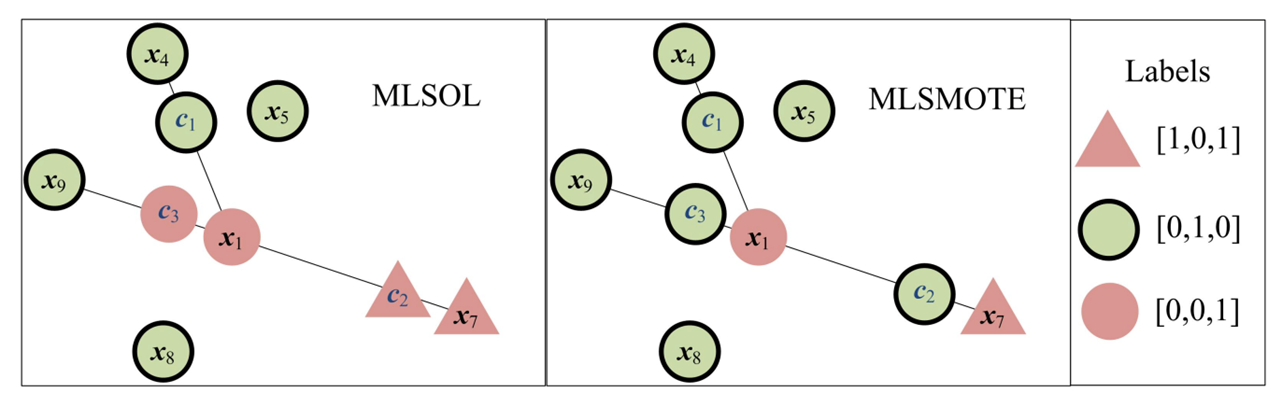
\includegraphics[width=1\textwidth]{3_State-of-the-art/fig/mlsmote_mlsol.png}
    \end{center}

    \caption{Distribution of prediction accuracy. \\ \textcolor{gray}{\fontsize{10}{0}\selectfont DOI: 110.1016/j.patcog.2021.108294}}
    \label{fig:mlsmote_mlsol}

    \end{figure*}
    
Table \ref{table:imbalanced}  presents a comparison of two methods, MLSMOTE and MLSOL, which are designed to address the issue of imbalanced data in multi-class classification. MLSMOTE enhances classifier performance by generating synthetic examples for each minority class label, thereby balancing the class distribution. Its primary advantage is the generation of these synthetic examples, which helps mitigate the imbalance. However, it has significant limitations: the synthetic samples generated might be related to the majority class, which can blur the distinction between classes, and the method struggles with overlapping classes, leading to potential misclassification. On the other hand, MLSOL systematically combats local imbalances by employing distinct sampling strategies for each label within a restricted neighborhood. This localized approach allows MLSOL to generate synthetic examples more precisely, addressing local imbalances effectively. Nonetheless, like MLSMOTE, MLSOL faces challenges with overlapping classes, which can result in misclassification in areas where class boundaries are not clear. Despite its advantages in handling local imbalances, the overlapping class issue remains a critical limitation for both methods, affecting their overall effectiveness in classification tasks.
\begin{table*}[!ht]

    \centering
    \caption{Comparison of the MLSMOTE and MLSOL methods.}
    \label{table:imbalanced}

    \small % Reduce font size
    \renewcommand{\arraystretch}{1} % Reduce cell padding
    \setlength{\tabcolsep}{4pt} % Reduce cell padding
    \setlength{\arrayrulewidth}{0.15mm}

    \begin{tabularx}{\textwidth}{|>{\centering\arraybackslash\bfseries}p{2cm}|
                                       >{\raggedright\arraybackslash}X|
                                       >{\raggedright\arraybackslash}X|
                                       >{\raggedright\arraybackslash}X|}
    \hline
    \textbf{Method} & \textbf{Theory} & \textbf{Advantages} & \textbf{Limitations} \\ 
    \hline
    \textbf{MLSMOTE} & 
    MLSMOTE significantly enhances classifier performance by generating synthetic examples for each minority class label. & 
    Generating synthetic examples for each minority class label. & 
    \begin{itemize}[leftmargin=*]
        \item Random synthetic samples may be related to the majority class.
        \item Overlapping classes.
    \end{itemize} \\ 
    \hline
    \textbf{MLSOL} & 
    MLSOL systematically combats local imbalances within the domain of multi-class classification by employing distinct sampling strategies for each label. & 
    Generating synthetic examples for each minority class label within a restricted neighborhood. & 
    \begin{itemize}[leftmargin=*]
        \item Overlapping classes.
    \end{itemize} \\
    \hline
    \end{tabularx}
    \end{table*}










\subsection{Emergence of new classes}
\label{sec:3_6_2_related_work_emergence}


Effectively detecting and adapting to new classes in streaming data is crucial for maintaining classification accuracy. Tree-based methods like SENCForest and SEEN utilize anomaly detection but face high false positive rates and runtime inefficiencies. SENNE improves detection performance using a nearest neighbor ensemble but suffers from longer runtimes due to the lack of an effective model retirement mechanism. The k-nearest Neighbor Ensemble-based method (KNNENS) addresses new class detection and known class classification using a k-nearest neighbor-based hypersphere ensemble and dynamic model updates. However, a critical limitation of these methods is their inadequate handling of concept drift, which is essential for detecting new classes and retraining the classification model. These methods represent the best closely related work for our proposal, which aims to build upon them by incorporating robust concept drift techniques for more adaptive and resilient classification systems.

Fig. \ref{fig:SENCForest} illustrates the SENCForest approach, which divides the space into three regions (normal, outlying, and anomaly) and detects emerging new classes (anomalies) using a calculated threshold path length. Fig. \ref{fig:SENNE} depicts the SENNE algorithm, where hyperplanes are drawn in three dimensions (x1, x2, and x3) for each class (Fig. \ref{fig:SENNE}a). New instances are then classified as emerging or known classes based on the rank of each class (Fig. \ref{fig:SENNE}b). Fig. \ref{fig:KENNE} presents the KNNENS algorithm, which draws hyperplanes for all class samples (Fig. \ref{fig:KENNE}a), and classifies new instances using a voting mechanism to determine if the instance is an emerging or known class (Fig. \ref{fig:KENNE}b). These visualizations highlight the operational differences between the SENNE and KNNENS algorithms in handling the classification of emerging and known classes.

\begin{figure*}[!ht]
    \centering
    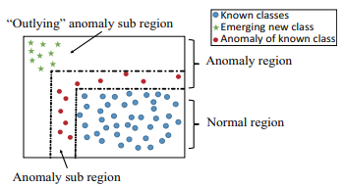
\includegraphics[width=0.85\textwidth]{3_State-of-the-art/fig/SENCForst.png}
    \caption{Overview of stream emerging new classes. \\
    \textcolor{gray}{\fontsize{10}{0}\selectfont DOI: 10.1109/TKDE.2017.2691702}}
    \label{fig:SENCForest}
\end{figure*}
    

\begin{figure*}[!ht]
    \begin{center}
        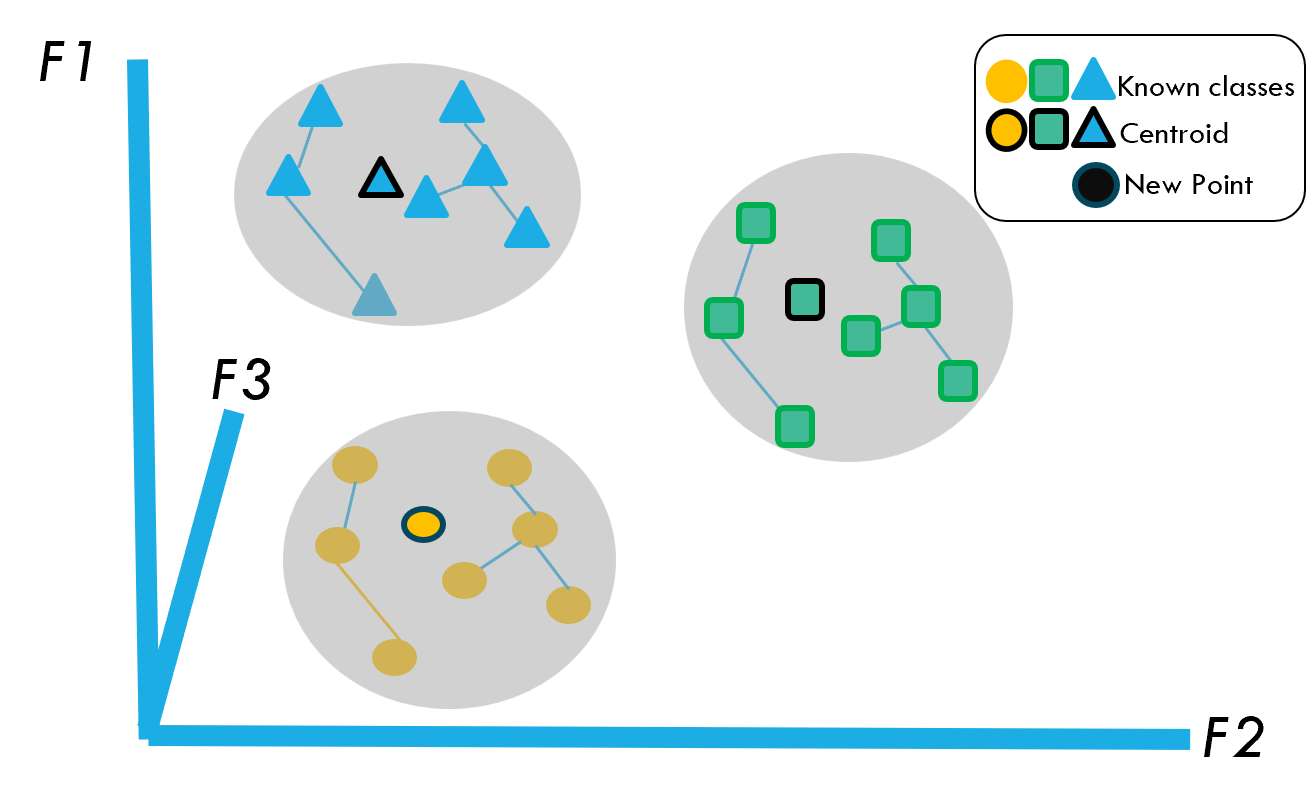
\includegraphics[width=.49\textwidth]{3_State-of-the-art/fig/senne0.png} 
        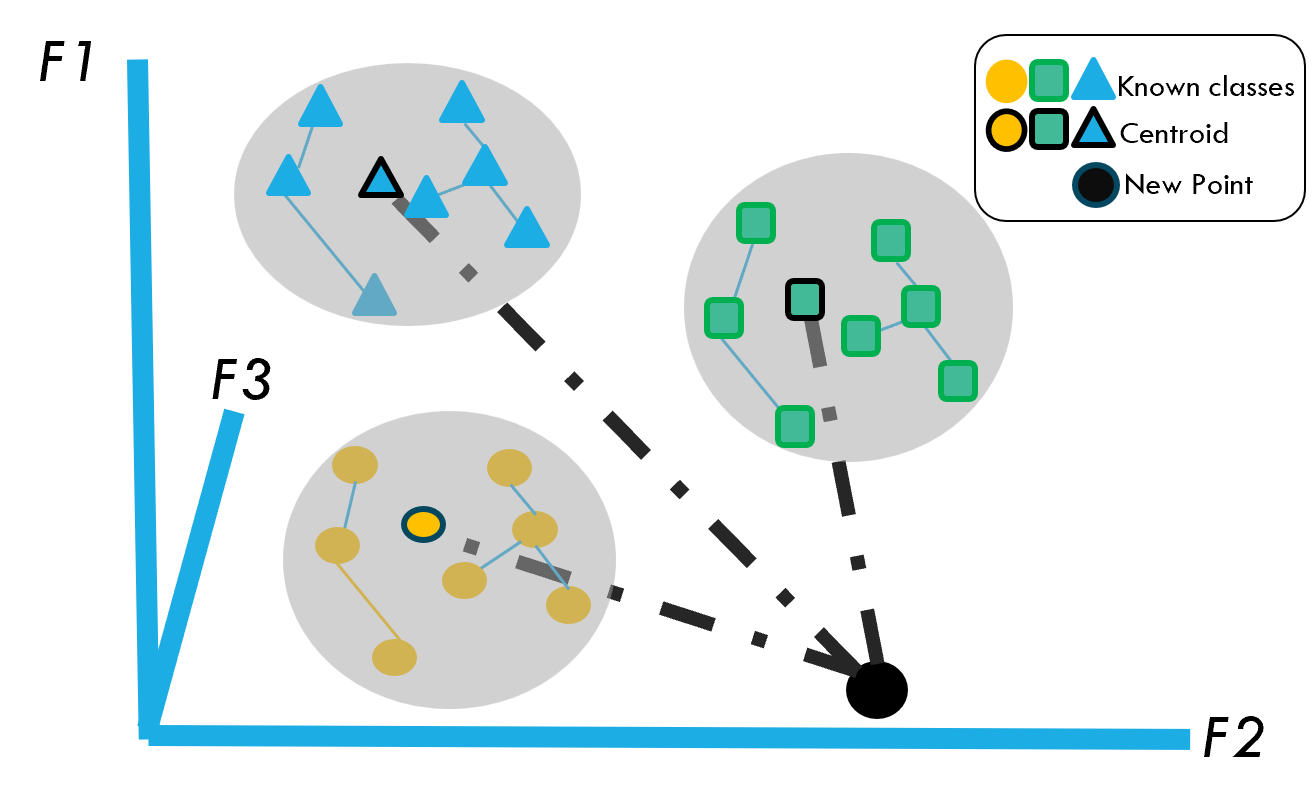
\includegraphics[width=.49\textwidth]{3_State-of-the-art/fig/senne.png} 
        (a)\hspace{6.5cm}(b)
    \end{center}
    \caption{Overview of the Stream Emerging Nearest Neighbor Ensemble (SENNE).}
    \label{fig:SENNE}
    \end{figure*}
    \vline
    \begin{figure*}[!ht]    
        \begin{center}
            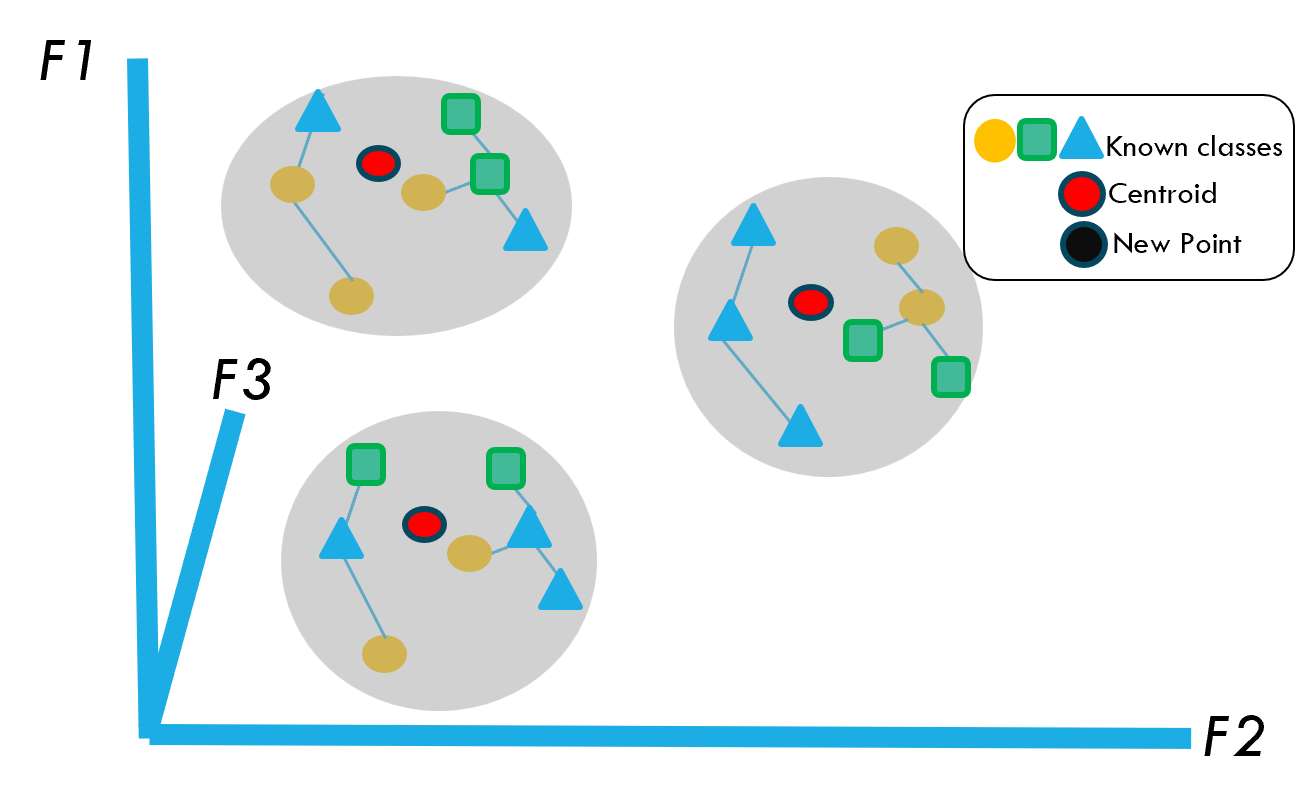
\includegraphics[width=.49\textwidth]{3_State-of-the-art/fig/kenne0.png} 
            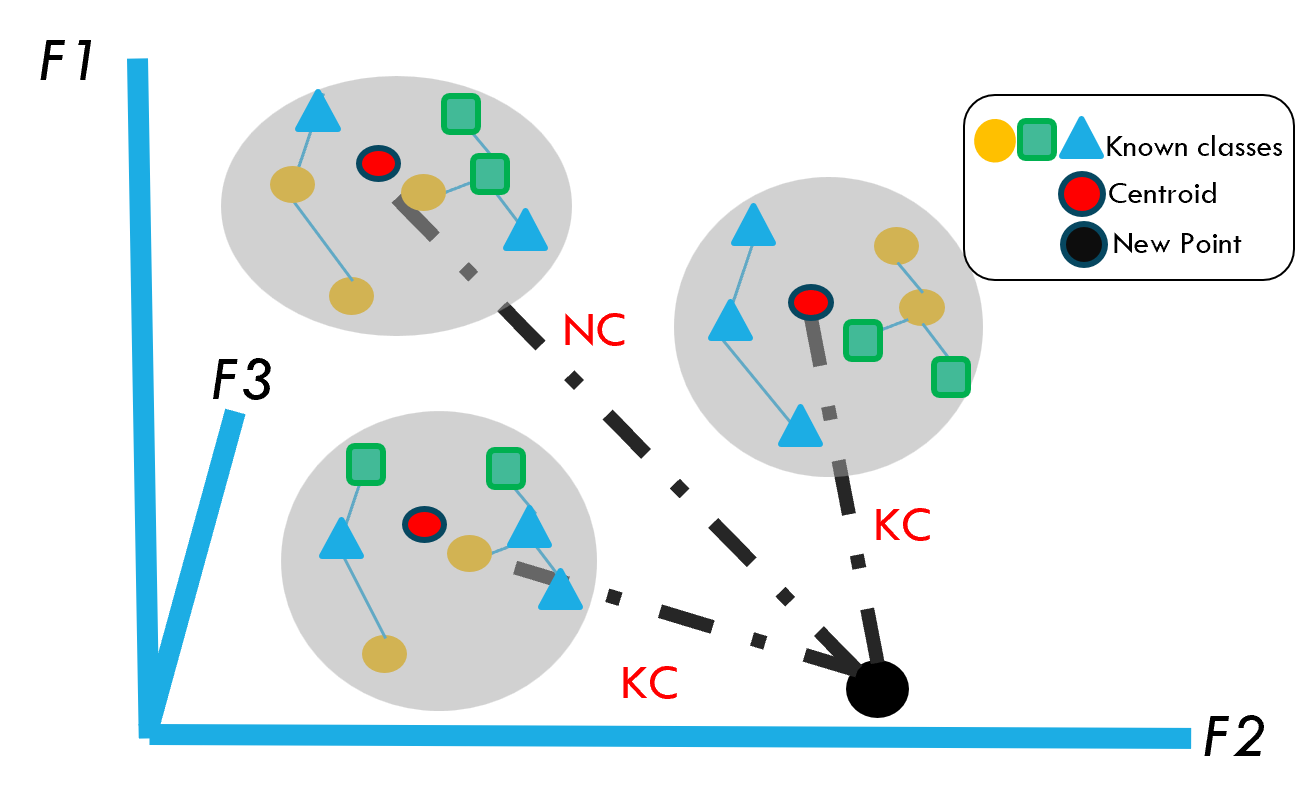
\includegraphics[width=.49\textwidth]{3_State-of-the-art/fig/kenne.png}
            (a)\hspace{6.5cm}(b)
            \end{center}
    
        \caption{Overview of the k-nearest Neighbor Ensemble-based (KENNE).}
        \label{fig:KENNE}
        \end{figure*}
        

        Table\ref{table:emerging} compares three methods for emerging class detection: SENCForest, SENNE, and KNNENS. SENCForest employs the anomaly detection method iForest for new class detection and uses a threshold path to identify anomalies, serving both as an unsupervised anomaly detector and a supervised classifier. However, it has a high potential for false positives and depends on a complex path length threshold. SENNE utilizes a nearest neighbor-based hypersphere of one class ensemble to explore local neighborhood information and sort distances, handling both low and high geometric distances between classes. Its limitations include the assumption that the distribution of known classes remains unchanged and it has lengthy update times. KNNENS employs a nearest neighbor-based hypersphere of all class ensembles to explore local neighborhood information, reducing false positives for new classes without needing true labels for model updates. However, like SENNE, it assumes that the distribution of known classes remains unchanged.

\begin{table*}[!ht]

    \centering
    \caption{Comparison of the SENCForest, SENNE, and KENNE methods.}
    \label{table:emerging}
    \small % Reduce font size
    \renewcommand{\arraystretch}{1} % Reduce cell padding
    \setlength{\tabcolsep}{4pt} % Reduce cell padding
    \setlength{\arrayrulewidth}{0.15mm}
    \begin{tabularx}{\textwidth}{|>{\centering\arraybackslash\bfseries}p{2cm}|
                                       >{\raggedright\arraybackslash}X|
                                       >{\raggedright\arraybackslash}X|
                                       >{\raggedright\arraybackslash}X|}
    \hline
    \textbf{Method} & \textbf{Theory} & \textbf{Advantages} & \textbf{Limitations} \\ 
    \hline
    \textbf{SENCForst} & 
    employs anomaly detection method iForest \cite{wang2010negative} for a new class detection and then applies threshold path to detect the anomalies. & 
    SENCForest serves as both an unsupervised anomaly detector and a supervised classifier.&
    \begin{itemize}[leftmargin=*]
        \item Potential for High False Positives.
        \item Dependency on Path Length Threshold (more complexity).
    \end{itemize} \\ 
    \hline
    \textbf{SENNE} & 
    nearest neighbor-based hypersphere of one class ensemble to explore local neighborhood information and sort distance to calculate distance. & 
    SENNE is able to handle both the low and high geometric distance between two classes in the feature space. & 
    \begin{itemize}[leftmargin=*]
        \item Assumes that the distribution of known classes remains unchanged.
        \item Take long time for update.
    \end{itemize} \\ 
    \hline
    \textbf{KENNE} & 
    nearest neighbor-based hypersphere of all class ensemble to explore local neighborhood information. & 
    KNNENS to reduce false positives for the new class. KNNENS does not require true labels to update the model. & 
    \begin{itemize}[leftmargin=*]
        \item Assumes that the distribution of known classes remains unchanged.
    \end{itemize} \\
    \hline
    \end{tabularx}
    \end{table*}













\subsection{Transfer Learning}
\label{sec:3_6_2_related_work_transfer}

In the realm of transfer learning, three prominent methods—CORAL, Melanie, and HE-CDTL—serve as closely related approaches to our proposed method. Correlation Alignment (CORAL) is an asymmetric transformation approach that aligns sub-space bases using second-order statistics. By employing a learned transformation matrix, CORAL projects source instances into the target domain, thereby minimizing domain discrepancies and reducing negative knowledge transfer. Melanie addresses the challenge of non-stationary environments through an online ensemble learning approach. It incrementally trains models from both source and target domains, dynamically adjusting their weights to handle concept drift, and combines these models via a weighted-sum approach as shown in Fig. \ref{coral_fig}. As Shown in Fig. \ref{cdtl_fig} This method can be extended to Concept Drift Transfer Learning (CDTL) by using an ensemble for chunk-based concept drift. HE-CDTL, designed explicitly for CDTL, leverages knowledge from source domains and historical time steps within the target domain to enhance learning performance. It utilizes a class-wise weighted ensemble for historical knowledge and implements AW-CORAL for extracting knowledge from source domains. The class-wise weighted ensemble allows individual classes to select historical knowledge independently, while AW-CORAL minimizes domain disparities and mitigates negative knowledge transfer. Extensive experiments have shown HE-CDTL to outperform baseline methods in addressing transfer learning challenges in the context of concept drift. Together, these methods provide a comprehensive framework for effective transfer learning in dynamic and evolving data environments.

Table\ref{table:transfer} compares three methods: CORAL, Melanie, and HE-CDTL. CORAL (Correlation Alignment) utilizes a learned transformation matrix and Singular Value Decomposition (SVD) to project source instances into the target domain, effectively minimizing domain discrepancy and reducing negative knowledge transfer. However, it faces challenges with non-stationary and heterogeneous data. Melanie (Multisource Online Transfer learning for Non-stationary Environments) addresses online learning problems where data in source and target domains are generated from non-stationary environments. Its advantages include considering online problems but it too is limited by the complexities of online learning and data heterogeneity. HE-CDTL (Class-wise Weighted and Domain-wise Ensemble) minimizes domain shift by aligning second-order statistics of source and target distributions, leveraging historical knowledge to reduce disparities between domains. Despite its strengths, it relies on the quality of the source domain and also struggles with heterogeneous data.
\begin{figure*}[!ht]

    \begin{center}
        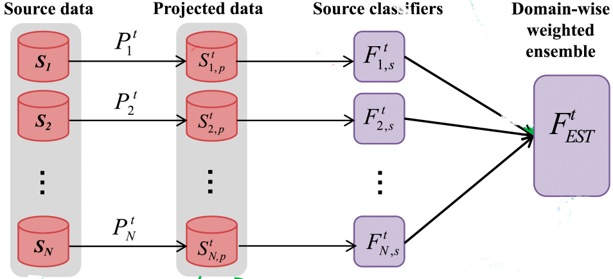
\includegraphics[width=.85\textwidth]{3_State-of-the-art/fig/coral.png} 
    \end{center}
    \caption{Overview of CORrelation ALignment (CORAL)}
    \label{coral_fig}
    \end{figure*}
    \begin{figure*}[!ht]    
        \begin{center}
            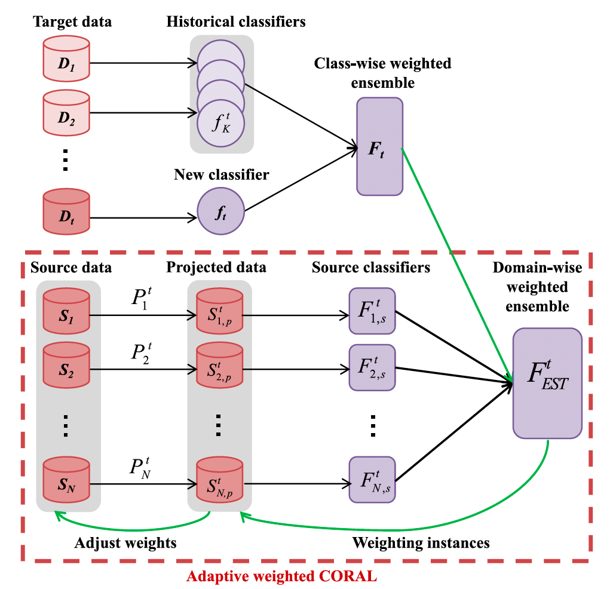
\includegraphics[width=.85\textwidth]{3_State-of-the-art/fig/cdtl.png} 
        \end{center}
        \caption{Overview of Concept Drift Transfer Learning (CDTL).}
        \label{cdtl_fig}

        \end{figure*}

\begin{table*}[!ht]
    \centering
    \caption{Comparison of the CORAL, Malanie, and CDTL methods.}
    \label{table:transfer}
    \small % Reduce font size
    \renewcommand{\arraystretch}{1} % Reduce cell padding
    \setlength{\tabcolsep}{4pt} % Reduce cell padding
    \setlength{\arrayrulewidth}{0.15mm}
    \begin{tabularx}{\textwidth}{|>{\centering\arraybackslash\bfseries}p{2cm}|
                                       >{\raggedright\arraybackslash}X|
                                       >{\raggedright\arraybackslash}X|
                                       >{\raggedright\arraybackslash}X|}
    \hline
    \textbf{Method} & \textbf{Theory} & \textbf{Advantages} & \textbf{Challenges} \\ 
    \hline
    \textbf{CORAL} & 
    Correlation Alignment (CORAL) uses a learned transformation matrix and Singular Value Decomposition (SVD)  to project the source instances into the target domain. & 
    CORAL can minimize domain discrepancy across
source and target domains, meanwhile reducing the negative
knowledge transfer. & 
    \begin{itemize}[leftmargin=*]
        \item Non-stationary environments.
        \item Heterogenous multisource.
    \end{itemize} \\ 
    \hline
    \textbf{Melanie} & 
    Multi-sourcE onLine TrAnsfer
learning for Non-statIonary Environments (Melanie). utilize the class-wise weighted . & 
It considers
an online problem in which the data in source and target
domains are generated from non-stationary environments. & 
    \begin{itemize}[leftmargin=*]
        \item Online Learning based only.
        \item Heterogenous multisource.
    \end{itemize} \\
    \hline
    \textbf{MLSOL} & 
    HE-CDTL uses the class-wise weighted and domain wise ensemble for historical knowledge and reduce the disparities between the source and target domains . & 
    HE-CDTL minimizes domain shift by aligning the second-order statistics of source and target distributions. & 
    \begin{itemize}[leftmargin=*]
        \item Depend on Source Domain Quality.
        \item Heterogenous multisource.
    \end{itemize} \\
    \hline
    \end{tabularx}
    \end{table*}

\section{Remarks} 
\label{sec:3_7_remartks}

By comparing the literature on ensemble learning for classification tasks, the proposals in this thesis differ from other studies in several ways:

\begin{enumerate}
    
    \item [-] As evident from our literature review on imbalanced streams, most studies have concentrated on generating synthetic samples while ignoring class overlap. \textit{To address this challenge}, we propose an approach to generate non-overlapping classes in imbalanced streams.

    \item [-] Oversampling techniques often perform inefficiently in the presence of concept drift. \textit{To tackle this issue}, we introduce a methodology that selects the oversampling technique based on the current and historical distribution of the stream chunks.
    
    \item [-] Our literature review on non-stationary environments reveals that most works focus on detecting emerging new classes while overlooking distribution changes. \textit{To overcome this challenge}, we propose a combined approach utilizing Dynamic Ensemble Selection (DES) to select the best classifier for each chunk based on stream distribution, k-means clustering, and concept drift to address both emerging new class detection and distribution changes.
    
    \item [-] In our literature review on transfer learning, we observed that most studies focus on homogeneous multisource transfer and neglect heterogeneous multisources in non-stationary environments. \textit{To resolve this issue}, we propose a combined approach integrating Dynamic Ensemble Selection (DES), Concept Drift Transfer Learning (CDTL), eigenvector techniques, and concept drift to address heterogeneous transfer learning in non-stationary environments.

\end{enumerate}



% imbalanced
% this file is called up by thesis.tex
% content in this file will be fed into the main document


\chapter{Dynamic Classification Ensembles for Handling Imbalanced
  Multiclass Drifted Data Streams}
  \label{chapter:4_Imbalanced_Multiclass}
  
  In recent years, the explosion of high-speed data streams has presented new challenges for machine learning models. Three critical
  issues that have emerged are concept drift, class imbalance, and class overlap. Concept drift refers to the phenomenon where the
  statistical properties of a data generation process change over time \cite{yang2021concept, dong2019multistream}. This signifies that the underlying concepts, relationships
  between variables, or data distribution can change, leading to a fundamental shift in the nature of data. Dealing with concept drift
  poses a fundamental challenge in machine learning and data mining. This can cause models trained on historical data to become
  inadequate when applied to new data affected by concept drift, leading to a decline in the model performance \cite{dong2019multistream}. To address this issue,
  concept drift detectors are used to identify changes in data stream distributions by leveraging information associated with classifier
  performance or the incoming data items themselves. These signals frequently prompt model updates, retraining, or substitution of an
  old model with a new one.
  In addition, class imbalance \cite{dong2019multistream, pan2009survey}, which is characterized by uneven class distribution, poses a challenge for traditional classifiers
  \cite{zhuang2020comprehensive}, particularly in multiclass scenarios where minority class samples are at risk of misclassification owing to their limited representation \cite{wang2018systematic}. Addressing imbalanced data classification requires specialized techniques to ensure accurate minority class classification without compromising the performance of the majority class \cite{sun2009classification, charte2015addressing, charte2015mlsmote}. This challenge becomes more daunting when minority class instances are scattered in unknown configurations, thereby increasing the likelihood of overfitting during the learning process. To
  address this issue, three primary methods are employed in the context of imbalanced data classification, which are effective in both
  binary and multiclass imbalance scenarios \cite{daniels2017addressing}. The first approach involves sampling methods that address class imbalance by either
  reducing the number of majority class instances (undersampling) or generating artificial minority class instances (oversampling)
  \cite{liu2018making,lopez2012analysis}. The second and third groups encompass adaptive algorithms and hybrid methods, respectively. Adaptive algorithms include
  one-class and cost-sensitive classification \cite{zhang2020towards}. Hybrid methods merge data preprocessing with classification techniques, often utilizing ensemble classifiers to effectively mitigate class imbalance and enhance classifier performance \cite{chawla2003smoteboost, wang2010negative, bhowan2012evolving}.
  Class overlap occurs when instances from different classes inhabit the same region in the data space \cite{galar2011review, cruz2018dynamic}. This overlap complicates the task of distinguishing between representative instances of various classes and posing performance challenges for traditional classifiers. This issue is commonly referred to as class overlap. Researchers have proposed class overlap undersampling
  techniques to address class imbalance problems \cite{kuncheva2000clustering}. These techniques aim to leverage local similarities among minority instances to
  identify potentially overlapping majority instances. Although these methods have demonstrated promising results in improving model
  performance on specific datasets, many of them rely heavily on nearest-neighbor approaches to detect overlapping regions around
  minority instances. This approach often neglects the global similarity within the overlapping domain, which can lead to local optimal
  values getting stuck during calculations. Furthermore, determining appropriate parameters for these models poses a significant
  challenge. If the parameter selection is too extensive, it may lead to the exclusion of valuable instances, while conservative parameters
  may overlook instances with overlap. This issue can significantly affect classifier performance, particularly when handling streams
  containing both a minority class and instances with class overlap. Therefore, both class imbalance and class overlap present significant
  challenges in the realm of data stream analyses. Consequently, addressing class imbalance is crucial in multiclass learning, leading to
  research efforts that focus on both concept drift and class imbalance challenges. Researchers have explored techniques such as DES and
  multiclass oversampling to address these issues.
  Dynamic classifier ensembles offer the unique ability to adapt their composition based on data characteristics, making them
  valuable in situations with evolving data conditions \cite{woloszynski2011probabilistic}. The aim of classifier ensemble selection is to identify the optimal subset of
  classifiers from a larger ensemble. A prominent approach in classifier ensemble selection is the overproduce-and-select strategy. This
  selection process is guided by diverse criteria, including individual performance measures, diversity metrics, meta-learning techniques,
  and performance-estimation approaches. Such optimization is particularly crucial in scenarios in which striking a balance between
  accuracy and computational resource constraints is paramount. There are two distinct approaches: static and dynamic approaches.
  Static selection involves assigning classifiers to predefined feature partitions, whereas dynamic selection adaptively selects classifiers
  based on their competency \cite{lysiak2014optimal}. Dynamic selection offers two choices: Dynamic Classifier Selection (DCS) and Dynamic Ensemble
  Selection (DES). DCS algorithms enable the selection of the most appropriate classifier for each data point, based on its local competencies. In contrast, DES focuses on selecting the optimal classifiers for each instance based on their competence within localized
  regions \cite{cruz2017meta, widmer1996learning, lu2016concept}. Competency assessment relies on a Dynamic SELection dataset (DSEL) containing labeled samples. Moreover,
  innovative techniques, such as the randomized reference classifier, introduce randomness into class supports to enhance adaptability
  in addressing the challenges related to imbalanced data.
  The main goal of this study is to formulate a precise classification approach that addresses changing conditions. Specifically, the
  first proposed approach aims to address scenarios where there is an uneven distribution among several classes, overlapping instances of
  classes, and instances where the fundamental concept of data evolves. To address these challenges, we employed dynamic classifier
  ensembles. These ensembles utilize oversampling techniques, implemented either on a global or local scale, as a preprocessing step to
  address class imbalance. Furthermore, we enhanced multiclass learning techniques to counteract class imbalance through method
  adaptation. 
  
  The remainder of this chapter is organized as follows: In Section \ref{sec:4_2_motivation}, we present the motivations and the contributions. The first proposed framework are discussed in detail in Section \ref{sec:4_first_proposed_approach}. The  experimental results and the discussion are presented in Sections \ref{sec:4_5_Expsetup}.
  
  
  \section{Motivations and Contributions} \label{sec:4_2_motivation}
  \begin{enumerate}[nosep]
    \item We introduce a classification approach that dynamically adjusts to multiclass imbalanced data, incorporates mechanisms for
    detecting concept drift, and optimizes classifier ensemble selection. The objective is to enhance the classification accuracy, specifically for multiclass imbalanced non-stationary streams.
   \item Additionally, we propose an adaptive method for the class imbalance issue, considering the data distributions and historical instances of class imbalance. This is particularly relevant in cases where class overlap occurs within the multiclass and drifted datan performance by selecting the most suitable oversampling method based on the unique characteristics of the data stream. 
    \end{enumerate}
\section{Proposed Methodology}
\label{sec:4_first_proposed_approach}

This section outlines the primary phases of the study, comprising three distinct stages. Following this introduction, the synthetic data-generator method is explored in detail, offering a comprehensive breakdown of the four essential steps. Our proposal aims to develop a robust approach designed to overcome the challenging domain of multiclass classification for imbalanced and drifting data streams. To achieve this objective, the proposed solution tackles the four primary challenges associated with developing this approach.
\begin{itemize}
	\item \textbf{Multi-class imbalanced streams:} This study focuses on addressing the widespread problem of imbalanced data streams in the context of multiple classes, aiming to tackle this issue using well-known techniques, particularly MLSMOTE and MLSOL.
	\item \textbf{Overlapping class:} A critical challenge involving class overlapping, which is known to substantially affect model performance \cite{cruz2017meta, widmer1996learning}, is also addressed. An adaptive method is introduced to generate non-overlapping synthetic instances, thereby enhancing the overall performance of the model.
	\item \textbf{Drifted streams:} First proposed approach integrates a concept drift detector to identify shifts in the underlying data distribution. This dynamic detection mechanism enables the model to promptly recognize changes and adjust its classifiers, thereby ensuring its effectiveness in handling drifting stream.
	\item \textbf{Classifier performance:} To enhance the classifier performance, tfirst approach employs Dynamic Ensemble Selection (DES). This technique creates a pool of classifiers and dynamically selects the most suitable classifier for each incoming data point, further improving classification performance and robustness.
\end{itemize}

\subsection{First Proposed Approach (PA1) Description}

First proposed approach is designed with three distinct phases that work together to improve its performance in managing multiclass imbalanced and drifting data streams. 
\begin{itemize}
	\item \textbf{DES phase (dynamic ensemble selection phase):} The first phase, known as the dynamic ensemble selection (DES) phase, is responsible for selecting the most appropriate classifier for the incoming data. This ensures that the selected classifier is well-suited for the current data chunk.
	\item \textbf{Drift detector phase:} The second phase of the first approach is the drift detector phase, which operates in real-time to continuously monitor the data stream. Its primary function is to identify any signs of concept drift, which indicates shifts in the underlying data distribution over time.
	\item \textbf{Synthetic data generator phase:} The final phase of the first approach is the synthetic data generator phase, which is dedicated to generating synthetic data for the minority classes. This step is crucial for addressing class imbalance by producing additional samples for underrepresented classes, thereby significantly enhancing the model's ability to accurately classify instances from minority classes.
	\item \textbf{Synthetic data generator phase:} The final phase of the first approach is the synthetic data generator phase, which is dedicated to generating synthetic data for the minority classes. This step is crucial for addressing class imbalance by producing additional samples for underrepresented classes, thereby significantly enhancing the model's ability to accurately classify instances from minority classes.
\end{itemize}
\begin{figure}[H]
	\centering
	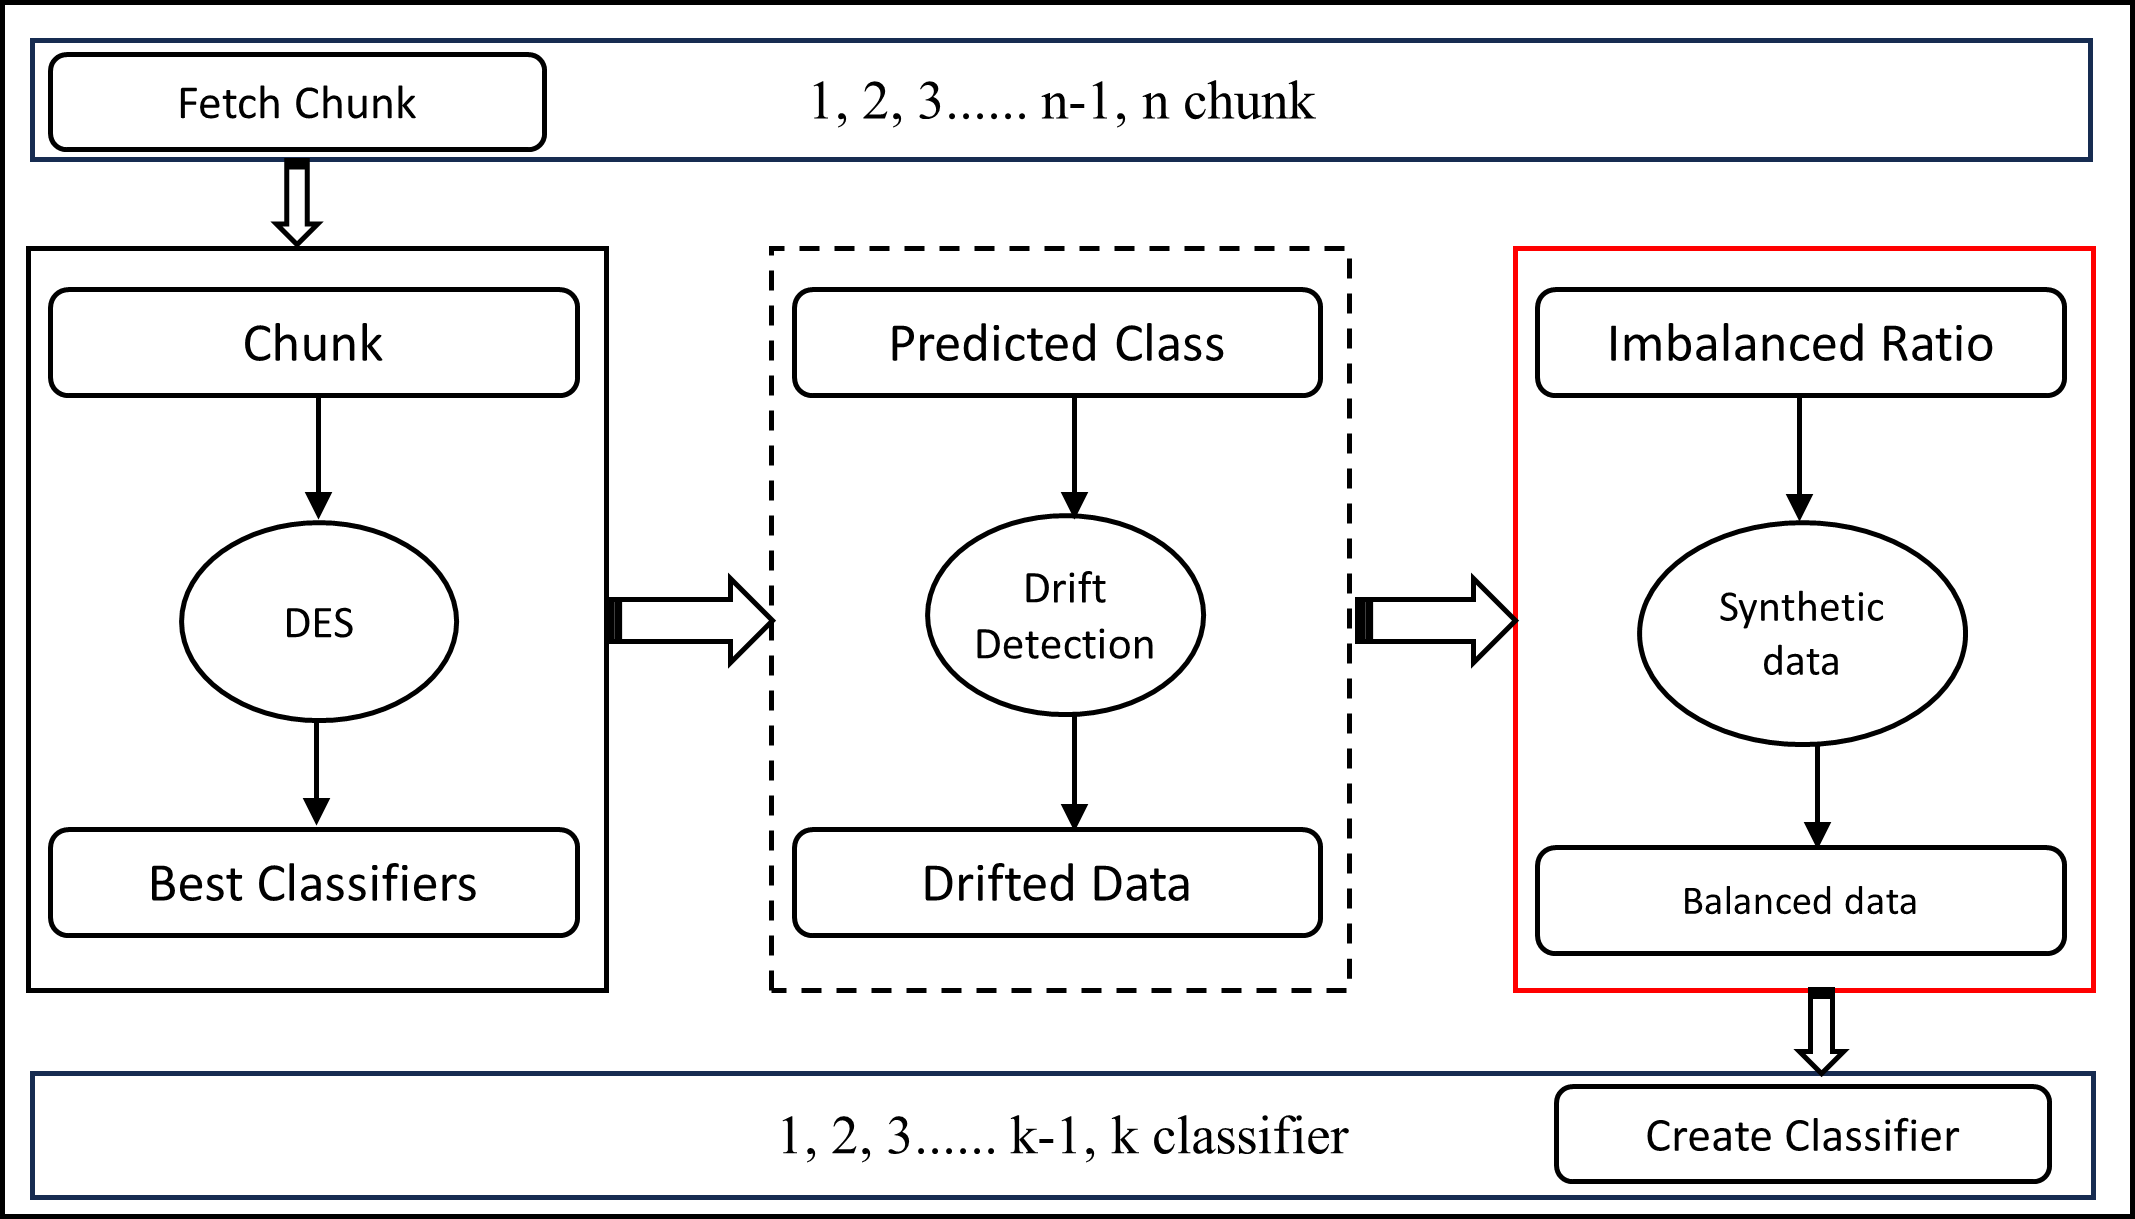
\includegraphics[width=1\linewidth]{4_Imbalanced/figures/approach_step_1.png}
	\caption{First Proposed Approach (PA1) for Imbalanced Multi-class Drifted Streams.}
	\label{fig:4_first_proposal_step_1}
\end{figure}
Specifically, as shown in Fig. \ref{fig:4_first_proposal_step_1}, the DES phase retrieves the current data chunk from the stream and applies the DES technique to select the most suitable classifiers for the received chunk. The selected classifiers were then passed to the second phase, where they were employed to predict the class of each instance within the received data chunk. Simultaneously, detectors like ADWIND or DDM are employed to monitor any occurrence of concept drift. If the discrepancy between the class frequency and standard deviation of the current chunk is significant, as described in reference \cite{gama2004learning}, and the imbalance ratio exceeds the average imbalance ratio, the current chunk is forwarded to the third phase, as indicated by the red rectangle in Fig. \ref{fig:4_first_proposal_step_1}. In the third phase, first proposed method uses a set of equations \ref{eq:4_first_proposal_1}\ref{eq:4_first_proposal_2}\ref{eq:4_first_proposal_3}
to identify minority classes. The initial equation computes the frequency of each class within the current chunk, where $i$ represents the current chunk, $c$ denotes the input class, and $y_i$ refers to the predicted class. The second equation determines the optimal frequency for each class based on the size of the chunk ($n$) and the number of classes in the current chunk($C$).

\begin{algorithm}[H]
	\caption{First Proposed Approach for Imbalanced Multi-class Streams.}
	\label{alg:4_alg_1}
	\KwIn{data stream, maximum classifiers pool size $\kappa$}
	\KwOut{Prediction $P$}
	\BlankLine
	$\psi, \Psi, \Omega, \mu \gets \emptyset$\;
	$\omega \gets 0$\;
	\For{stream have chunk}{
		\eIf{$a$ is the First chunk}{
			$k \gets$ \texttt{trainingNewClassifier}($a$)\;
			$P \gets$ \texttt{getPrediction}($a, k$)\;
		}{
			$k \gets$ \texttt{DES}($a, \Psi$)\;
			$P \gets$ \texttt{getPrediction}($a, k$)\;
			$\psi \gets$ \texttt{conceptDriftDetector}($P$)\;
			\If{$\psi > 0$}{
				$\Omega \gets$ get classes frequency according to Eq.1\;
				$\omega \gets$ best frequency according to Eq.2\;
				$\mu \gets$ get minority classes according to Eq.3\;
				$b \gets$ utilize $a$ and $\mu$ to get the synthetic data according to Algorithm \ref{alg:4_alg_2}\;
				trainingData $\gets a + b$\;
				$k \gets$ \texttt{trainingNewClassifier}(trainingData)\;
				$\Psi \gets \Psi + k$\;
				\If{$\Psi > \kappa$}{
					\texttt{removeWorstClassifier}($\Omega$)\;
				}
			}
			$P \gets$ \texttt{getPrediction}($a, k$)\;
		}
	}
	\Return{$P$}
	\end{algorithm}

Finally, the third equation identifies the classes as minority classes if their frequency deviates significantly from the standard deviation of the current chunk, where $sd_c$ represents the standard deviation of the class instances, and $frq_i$ refers to the standard deviation of the current chunk.
Figure \ref{fig:4_first_proposal_step_2} shows that phase These identified minority classes are then fed into the synthetic data generator phase, which increases the minority class samples to balance any imbalanced chunks. This ensures optimal performance for the new classifiers. Algorithm  \ref{alg:4_alg_1} provides a comprehensive outline of the process of the first proposed approach, which is the main contribution of this study and is designed to effectively address multiclass imbalanced and drifting data streams, uses streaming data as input, and systematically executes each step within the approach. The outcome of this process is the classification prediction generated using the first proposed approach.

\subsection{Synthetic Data Generator Phase Description}

Figure \ref{fig:4_first_proposal_step_2} presents a comprehensive overview of the synthetic data generator phase, which is an essential component responsible for generating synthetic samples by considering both data distribution and historical chunk behaviors. This phase has several advantages and can perform a wide range of tasks.
\begin{figure}[H]
	\centering
	
\includegraphics[width=1\linewidth]{4_Imbalanced/figures/approach_step_2.png}
	\caption{Flow Diagram of the Synthetic Data Generator.}
	\label{fig:4_first_proposal_step_2}
\end{figure}
\begin{itemize}
	\item \textbf{Similar chunk analysis:} Initially, the phase analyzes the current chunk distribution and identifies a similar chunk from historical data. This analysis forms the basis for generating synthetic samples that align with prevailing distribution patterns.
	\item \textbf{Oversampling method selection:} This phase utilizes the knowledge of the oversampling technique applied to the identified similar chunk. Consequently, it employs an alternative oversampling technique, using MLSMOTE and MLSOL, to create the most effective synthetic data. This step is designed not only to optimize the current classification but also to preemptively address potential drifts in similar future chunks.
	\item \textbf{Class overlap validation:} This step involves generating synthetic samples for the minority classes to effectively address the issue of minority classes and consequently enhance the classifier performance. The process utilizes the K-Nearest Neighbor (KNN) algorithm, as applied in \cite{lu2016concept}, to identify overlaps between newly generated data instances and existing instances. If overlaps are detected, the first proposed approach iteratively removes these samples because their presence can potentially diminish the overall classifier performance \cite{cruz2017meta, widmer1996learning}. Consequently, the first proposed approach generates alternative samples to address this challenge and preserve the primary objectives of the synthetic data generator step.
	\item \textbf{Continuous refinement:} This process iterates until it successfully generates high-quality synthetic data that aligns with the data distribution, minimizes overlap, and mitigates potential concept drift. The generated data were subsequently utilized in the training phase to improve classifier performance.
\end{itemize}
\begin{algorithm}[H]
	\caption{Synthetic Data Generator Algorithm.}
	\label{alg:4_alg_2}
	\KwIn{Minority classes $\mu$, current chunk $a$, sample size $\eta$, historical chunks $h$}
	\KwOut{Generated data $b$}
	$b \gets \emptyset$\;
	$f \gets \text{MLSMSOTE}$\;
	$knn \gets \text{kNearestNeighbor}(a)$\;
	$chunk \gets \text{similarChunk}(a, h)$\;
	$f \gets \text{similarChunkOverSamplingMethod}(chunk)$\;
	\If{$f = \text{MLSMSOTE}$}{
		$f \gets \text{MLSOL}$\;
	}
	\Else{
		$f \gets \text{MLSMSOTE}$\;
	}
	\While{$|b| < \eta$}{
		$p \gets \text{generateSyntheticPoint}(\mu, f)$\;
		$similarPointsClass \gets \text{KNN.getKneighbor}(b)$\;
		\If{$similarPointsClass = \mu$}{
			$b \gets b \cup \{p\}$\;
		}
	}
	\Return $b$\;
	\end{algorithm}
In Algorithm \ref{alg:4_alg_2}, also known as the Synthetic Data Generator, three essential elements are inputted: the minority class samples, the current data chunk, and the desired size for generating synthetic data. The primary objective of this algorithm is to produce synthetic data samples. To achieve this, the KNN algorithm is employed to identify any overlapping instances within the current chunk (Line 3). This algorithm utilizes two specific techniques, MLSMOTE \cite{gama2004learning} and MLSOL \cite{liu2017regional}. MLSMOTE was chosen for its introduction of randomness during instance generation, reducing its reliance on the local characteristics and distribution of the minority class. This randomization diminishes the likelihood of producing overlapping instances, particularly in cases where minority class instances are situated in overlapping regions. In contrast, MLSOL considers the local behavior of minority classes, resulting in synthetic points that closely resemble the minority class. This approach significantly improves the performance of the classifier (lines 4-10). Additionally, in this algorithm, specifically from lines 11 to 17, these lines are dedicated to generating synthetic instances that ensure non-overlap with existing classes. This procedure depends on the selected oversampling method and utilizes the KNN algorithm to guarantee that the generated instances do not overlap with the existing ones.


	\section{Mathematical Foundation for PA1}
	\label{sec:math_foundation_pa1}
	
	The mathematical foundation for PA1 involves key equations designed to identify and classify data chunks based on class frequencies and distributions. These equations are fundamental to analyzing imbalanced data streams effectively.
	
	Equation \ref{eq:4_first_proposal_1} calculates the frequency of a specific class \(c\) within a data chunk. For each instance \(y_i\), the frequency \(frq_{c}\) is incremented if the instance belongs to class \(c\):  
	\begin{equation}
	\label{eq:4_first_proposal_1}
	frq_{c} = \sum_{i=1}^{\text{chunk size}} 
	\begin{cases} 
	1, & \text{if } y_i = c \\
	0, & \text{otherwise}
	\end{cases}, \quad i = 1, 2, 3, \dots \text{chunk size}.
	\end{equation}
	
	Equation \ref{eq:4_first_proposal_2} defines the \textit{best frequency} for a chunk, \(freq_n\), as the proportion of instances \(n\) relative to the total number of classes \(C\):  
	\begin{equation}
	\label{eq:4_first_proposal_2}
	\text{best } freq_{n} = \frac{|n|}{|C|}.
	\end{equation}
	
	Finally, Equation \ref{eq:4_first_proposal_3} determines the type of each class in the chunk (\textit{Minority} or \textit{Majority}) by comparing the difference between the standard deviation (\(sd_c\)) and the class frequency (\(frq_i\)) against the best frequency of the chunk (\(freq_{\text{chunk}}\)):  
	\begin{equation}
	\label{eq:4_first_proposal_3}
	\text{classes type}_{\text{chunk}} = \sum_{c=1}^{C} 
	\begin{cases} 
	\text{Minority,} & \text{if } diff(sd_c - frq_i) > \text{best } freq_{\text{chunk}} \\
	\text{Majority,} & \text{otherwise}.
	\end{cases}
	\end{equation}
	
	These equations collectively enable precise identification of class types within data chunks, forming a critical component of the PA1 framework.
	
	
%%%%%%%%%%%%%%%%%%%%%%%%%%%%%%%%%%%%%%%%%%%%%%%
%
%   Families of Traffic Forecasting Problems
%
%%%%%%%%%%%%%%%%%%%%%%%%%%%%%%%%%%%%%%%%%%%%%%%

%\usepackage{cite}
%\usepackage{multirow}
%\usepackage{rotating} 
%\usepackage[table,xcdraw]{xcolor}
%\usepackage{float}
%\usepackage[utf8]{inputenc}
%\usepackage{amsmath,amssymb,amsfonts}
%\usepackage{algorithmic}
%\usepackage{graphicx}
%\usepackage{textcomp}
%\usepackage{rotating}
%\usepackage{verbatim}


\section{Experimental Results}
\label{sec:4_5_Expsetup}

The objective of the experiments conducted in this study was to evaluate the efficacy of multiclass oversampling techniques in enhancing the performance of the proposed method in imbalanced drifted multiclass classification streams. Our primary goal was to develop a novel approach that combines Dynamic Ensemble Selection (DES) to improve classification accuracy and robustness in such streams. These experiments yielded valuable insights that could further refine the performance of the proposed approach and its ability to effectively handle imbalanced data streams. These findings provide a better understanding of the capabilities of the proposed approach and offer insights into an optimal strategy for tackling minority class issues and concept drift in imbalanced data streams. This study contributes to the advancement of stream mining techniques for generating more accurate and robust classification models in dynamic data stream environments. By addressing the challenges posed by minority classes and concept drift, this study offers valuable insights for improving the performance of the proposed approach and enhancing the overall efficiency of stream mining. The two main questions to be answered are:

\begin{itemize}
  % \setlength{\itemindent}{-.5in}
  
      \item $\pmb{Q_1}$: What is the impact of reduced and consistent data on the performance of ensemble learning?
      \item  $\pmb{Q_2}$: Is it possible with the search capability of swarm intelligence to enhance the combination of classifiers? 
  \end{itemize}

\subsection{Experimental setup}
The evaluation of the proposed method incorporated the utilization of various metrics such as recall, precision, specificity, f1 score, balanced accuracy score (BAC), and geometric mean score (G-mean) \cite{bu2016pdf}. The experimental protocol utilized for evaluation was the test-then-train approach \cite{venkatasubramanianinformation}, where the classification classifier was trained on a specific data chunk and subsequently evaluated on the subsequent one. The chunk size was standardized for all utilized data streams to 2,000 instances. We employed four classification classifiers as base estimators: K-Nearest Neighbor (KNN), Support Vector Machine (SVM), Gaussian Naive Bayes (GNB), and Hoeffding Tree (HT), as implemented in scikit-learn \cite{frias2014online}. A pool of classifiers was constructed with a maximum size of L = 8, where the DES selected the best classifier for each chunk. If the pool surpassed the set threshold (L), the classifier with the lowest performance was eliminated. The experiments were conducted using Python programming language, and the source code was publicly available on GitHub\footnote{\url{https://github.com/Amadkour/dynamic__classification_ensembles_for_handling_imbalanced_multi-class_drifted_data_streams.git}} . We conducted a comparison between multiclass oversampling techniques (MLSMOTE and MLSOL) and our proposed approach to demonstrate the effectiveness of our contribution. Additionally, we conducted these experiments using two different concept drift detectors, ADWIN \cite{storkey2008training} and DDM \cite{losing2016knn}, to demonstrate the adaptability and robustness of our proposed approach across varying drift detectors.

\subsection{Data Streams}
In this study, the proposed approach was assessed using various datasets including benchmark datasets, a real application stream dataset, and synthetic data streams. The Stream-learn Python library was used to conduct the evaluations \cite{dries2009adaptive}. Table \ref{tab:4_first_proposal_result_table_1} illustrates the benchmark dataset employed in this study, which consists of the Covertype dataset containing 40 features, seven classes, and 581,010 instances. For real application stream evaluation, the Sensor stream dataset was used, which consisted of five features, 58 classes, and 392,600 instances. This represents a real-world application scenario and provides valuable insights into the performance of the proposed approach in practical settings. Synthetic datasets were generated using Scikit-learn Python library to evaluate the performance of the proposed approach. The synthetic dataset was designed to simulate data streams and comprised 10 features and four classes divided into 200 chunks of 2,000 instances each. The performance of the proposed approach was systematically evaluated using these datasets and a stream-learn library. These evaluations provided insights into the effectiveness of the proposed approach in handling different types of data streams, including benchmark datasets, real application streams, and synthetic data streams.

\begin{table}[h!]
  \centering
  \resizebox{\textwidth}{!}{
  \begin{tabular}{|l|c|c|c|}
  \hline
  \textbf{Dataset} & \textbf{Number of Features} & \textbf{Number of Classes} & \textbf{Number of Instances} \\ \hline
  Covertype dataset\footnote{\url{http://archive.ics.uci.edu/dataset/31/covertype}} & 40 & 7 & 581,010 \\ \hline
  Sensor Stream dataset\footnote{\url{https://www.cse.fau.edu/~xqzhu/Stream/sensor.arff}} & 5 & 58 & 392,600 \\ \hline
  Synthetic stream & 8 & 3 & 200,000 \\ \hline
  \end{tabular}
  }
  \caption{Characteristics of the datasets used in the experiments.}
  \label{tab:4_first_proposal_result_table_1}
  \end{table}

\subsection{Analysis of Experimental Results}
The performance of the proposed framework was comprehensively assessed on multiple data streams, considering two distinct concept drift detectors, ADWIN and DDM. To ensure thorough evaluation, six key performance metrics—F1 score, recall, precision, G-mean, specificity, and balanced accuracy—were carefully presented using two visualization diagrams: radar and line. A radar diagram was strategically utilized to provide an overview that effectively depicted the performance of each algorithm across the six metrics. The mean value of each metric was calculated to present the overall performance of each method (MLSMOTE, MLSOL, PA). It is important to note that the PA is represented by red lines.
\subsubsection{Results on the Benchmark Stream}
The results of the mentioned methods (MLSMOTE, MLSOL, PA) applied to the Covertype dataset are presented in Fig. \ref{fig:4_first_proposal_result_exp_1}
, utilizing ADWIN as the drift detector. The radar diagram shows that the metric values were between 0.8 and 1.0. MLSOL exhibited the highest precision, whereas MLSOTE and PA had nearly identical values. However, PA excels in other metrics, whereas MLSMOTE has the lowest values. The line diagram in Fig. \ref{fig:4_first_proposal_result_exp_1}
shows the classification accuracy across 100 data chunks using the specificity metric for the methods in each chunk. Notably, all methods exhibit suboptimal accuracy during the first 20 chunks. However, a noticeable improvement was observed beyond this initial phase. The key factor driving this improvement was the expansion of the classifier pool, which now encompasses a growing number of classifiers. This expansion enables the Dynamic Ensemble Selection (DES) technique to become more proficient in selecting the most suitable classifier for each incoming chunk. Consequently, accuracy experienced a significant boost in later chunks, reflecting the adaptability and effectiveness of the ensemble approach. From chunk 20 to the last chunk, PA achieved the highest accuracy, whereas MLSMOTE recorded the lowest accuracy. PA's superior performance of the PA is credited to its use of historical chunks to generate optimal nonoverlapping samples, thereby effectively training the pool classifiers. In Fig. \ref{fig:4_first_proposal_result_exp_2}
, the same dataset is employed with the DDM functioning as the drift detector. The radar plot illustrates results comparable to those of the prior experiment, whereas the line diagram underscores PA's supremacy in most chunks. However, it also reveals that all approaches demonstrate diminished performance, in contrast to Fig. \ref{fig:4_first_proposal_result_exp_1} (ADWIN), suggesting that ADWIN surpasses DDM when utilized in the Covertype data stream.


\begin{figure}[!ht]
	\centering
	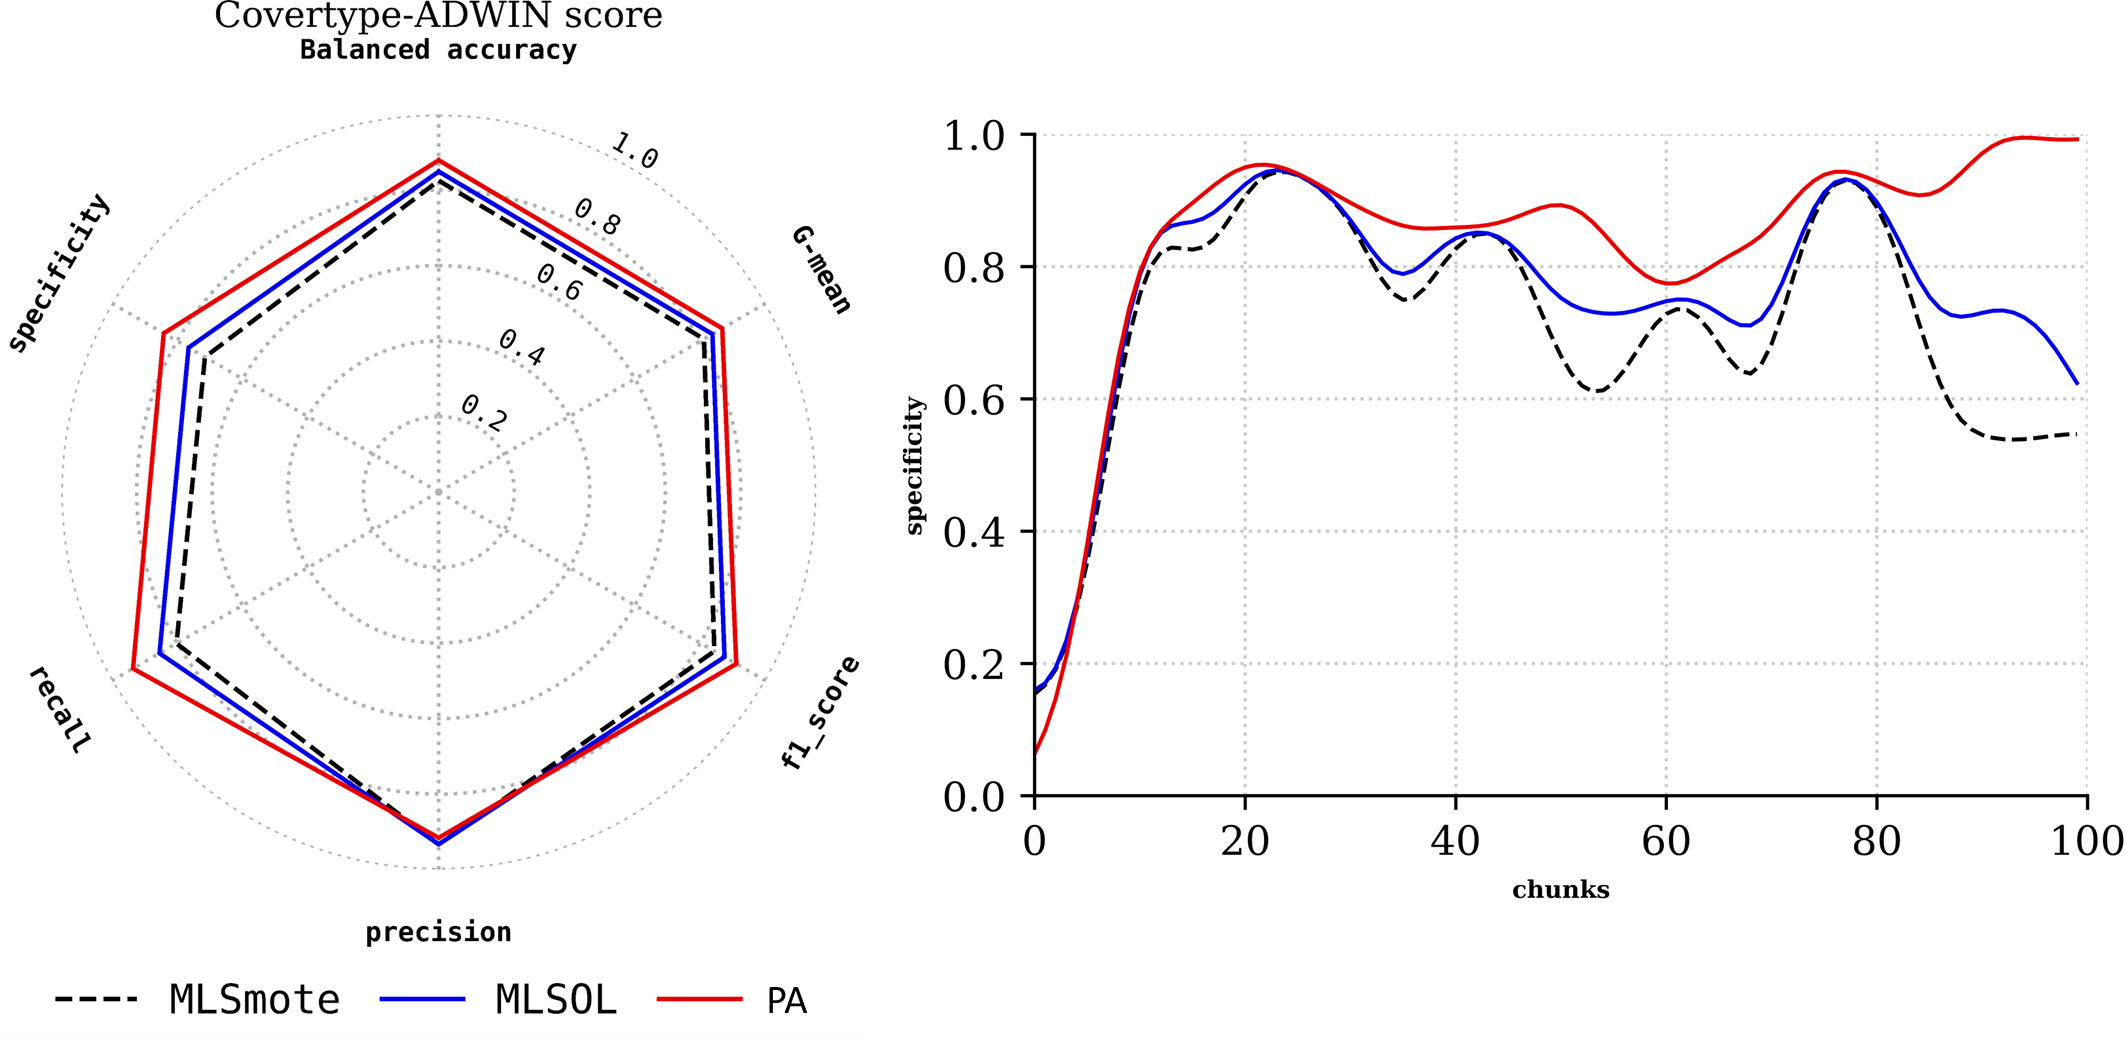
\includegraphics[width=1\linewidth]{4_Imbalanced/figures/exp_1.png}
	\caption{Performance of the Proposed Approach (PA), MLSMOTE, and MLSOL techniques on the Covertype Benchmark dataset using the ADWIN concept drift detector.}
	\label{fig:4_first_proposal_result_exp_1}
\end{figure}

\begin{figure}[!ht]
	\centering
	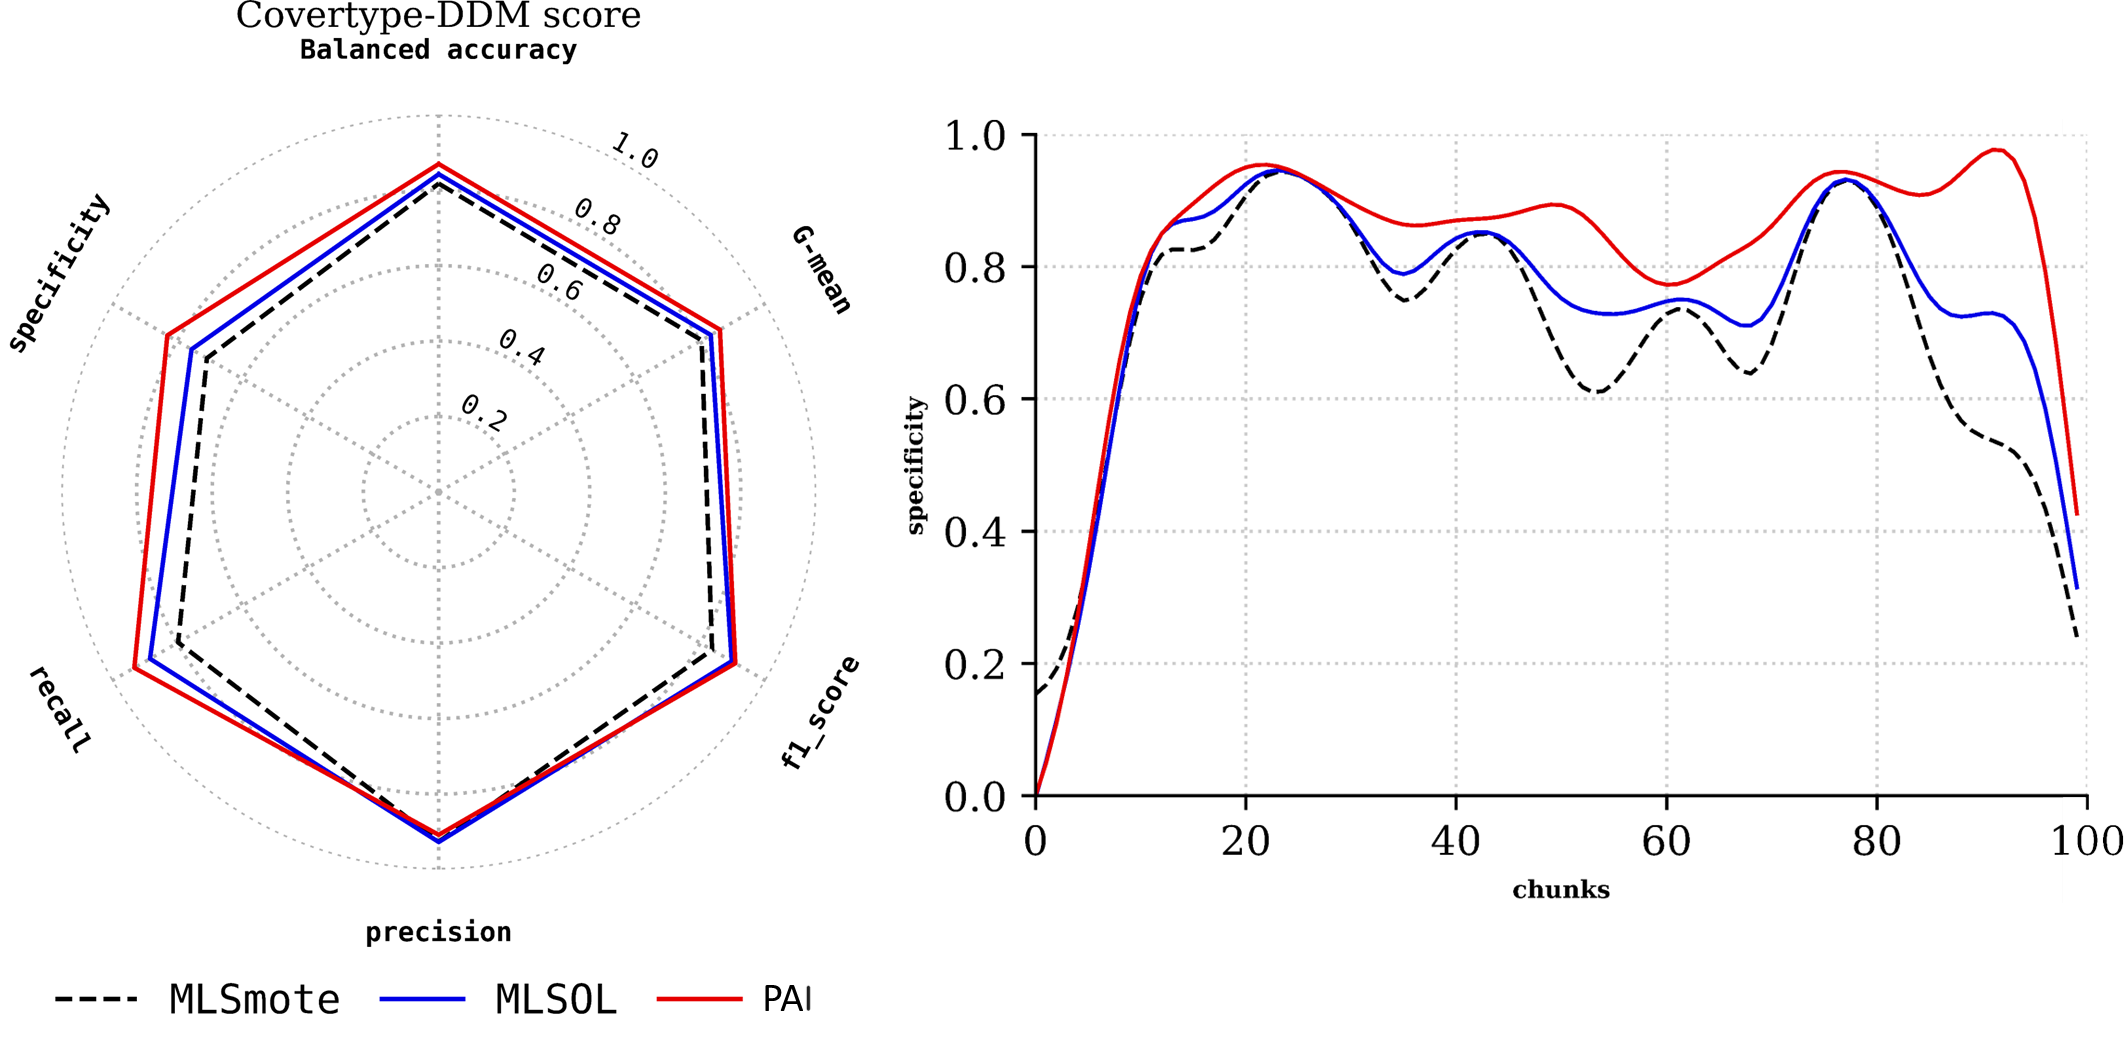
\includegraphics[width=1\linewidth]{4_Imbalanced/figures/exp_2.png}
  \caption{Performance of the Proposed Approach (PA), MLSMOTE, and MLSOL techniques on the Covertype Benchmark stream using the DDM concept drift detector.}
	\label{fig:4_first_proposal_result_exp_2}
\end{figure}

\subsubsection{Results on the Real Application Stream}
Fig. \ref{fig:4_first_proposal_result_exp_3} illustrates the outcomes of employing the three methods on the Sensor data stream using ADWIN as the drift detector. The radar graph depicts metric values ranging from 0.6 to 0.8, which indicate the pronounced drift and imbalance of the Sensor stream. In terms of the precision and recall metrics, the three methods exhibited almost identical values, whereas PA stood out in the other metrics. In contrast, MLSMOTE and MLSOL displayed similar values. By examining the line graph in Fig. \ref{fig:4_first_proposal_result_exp_3}
, it is evident that during the initial 30 chunks, PA's performance of PA might be suboptimal in some instances because of the limited number of classifiers in the pool. However, after the first 30 chunks, the performance significantly improved with the addition of more classifiers. In the same graph, PA consistently achieved the highest performance across all chunks, whereas MLSMOTE exhibited lower performance in certain chunks, and MLSOL exhibited lower performance in the other chunks. In Fig. \ref{fig:4_first_proposal_result_exp_4}, using the same dataset with the DDM as the drift detector, the radar plot metrics indicate lower results compared to the previous experiment. Nonetheless, the line graph underscores PA's dominance of PA in most chunks, although all methods exhibit nearly identical performance across the entire set of chunks. Overall, the performance of all the methods in Fig. \ref{fig:4_first_proposal_result_exp_4} is inferior to that in Fig. \ref{fig:4_first_proposal_result_exp_3} (ADWIN), which highlights ADWIN's superiority of ADWIN over DDM when applied to the Sensor data stream. 


\begin{figure}[!ht]
	\centering
	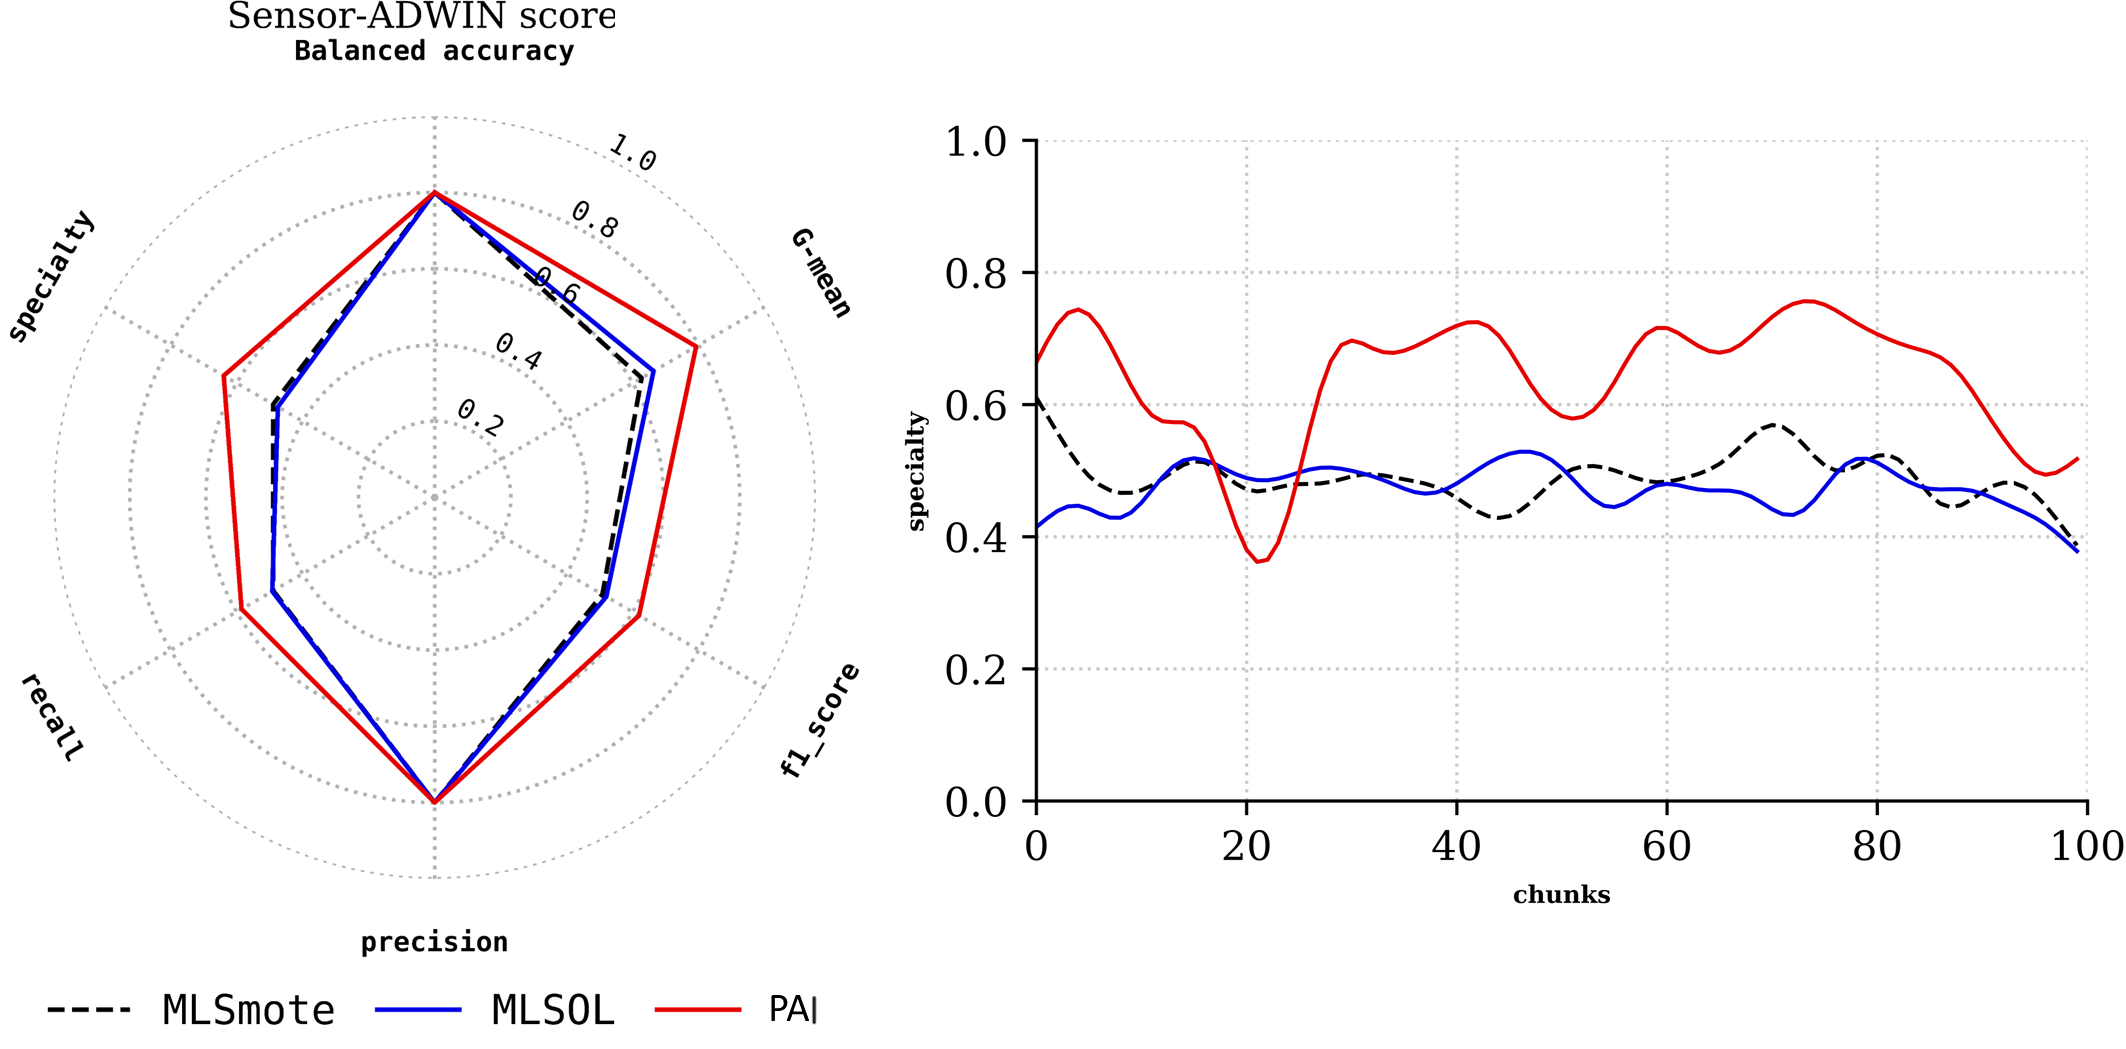
\includegraphics[width=1\linewidth]{4_Imbalanced/figures/exp_3.png}
  \caption{Performance of the Proposed Approach (PA), MLSMOTE, and MLSOL techniques on the Sensor real application stream using the ADWIN concept drift detector.}
	\label{fig:4_first_proposal_result_exp_3}
\end{figure}

\begin{figure}[!ht]
	\centering
	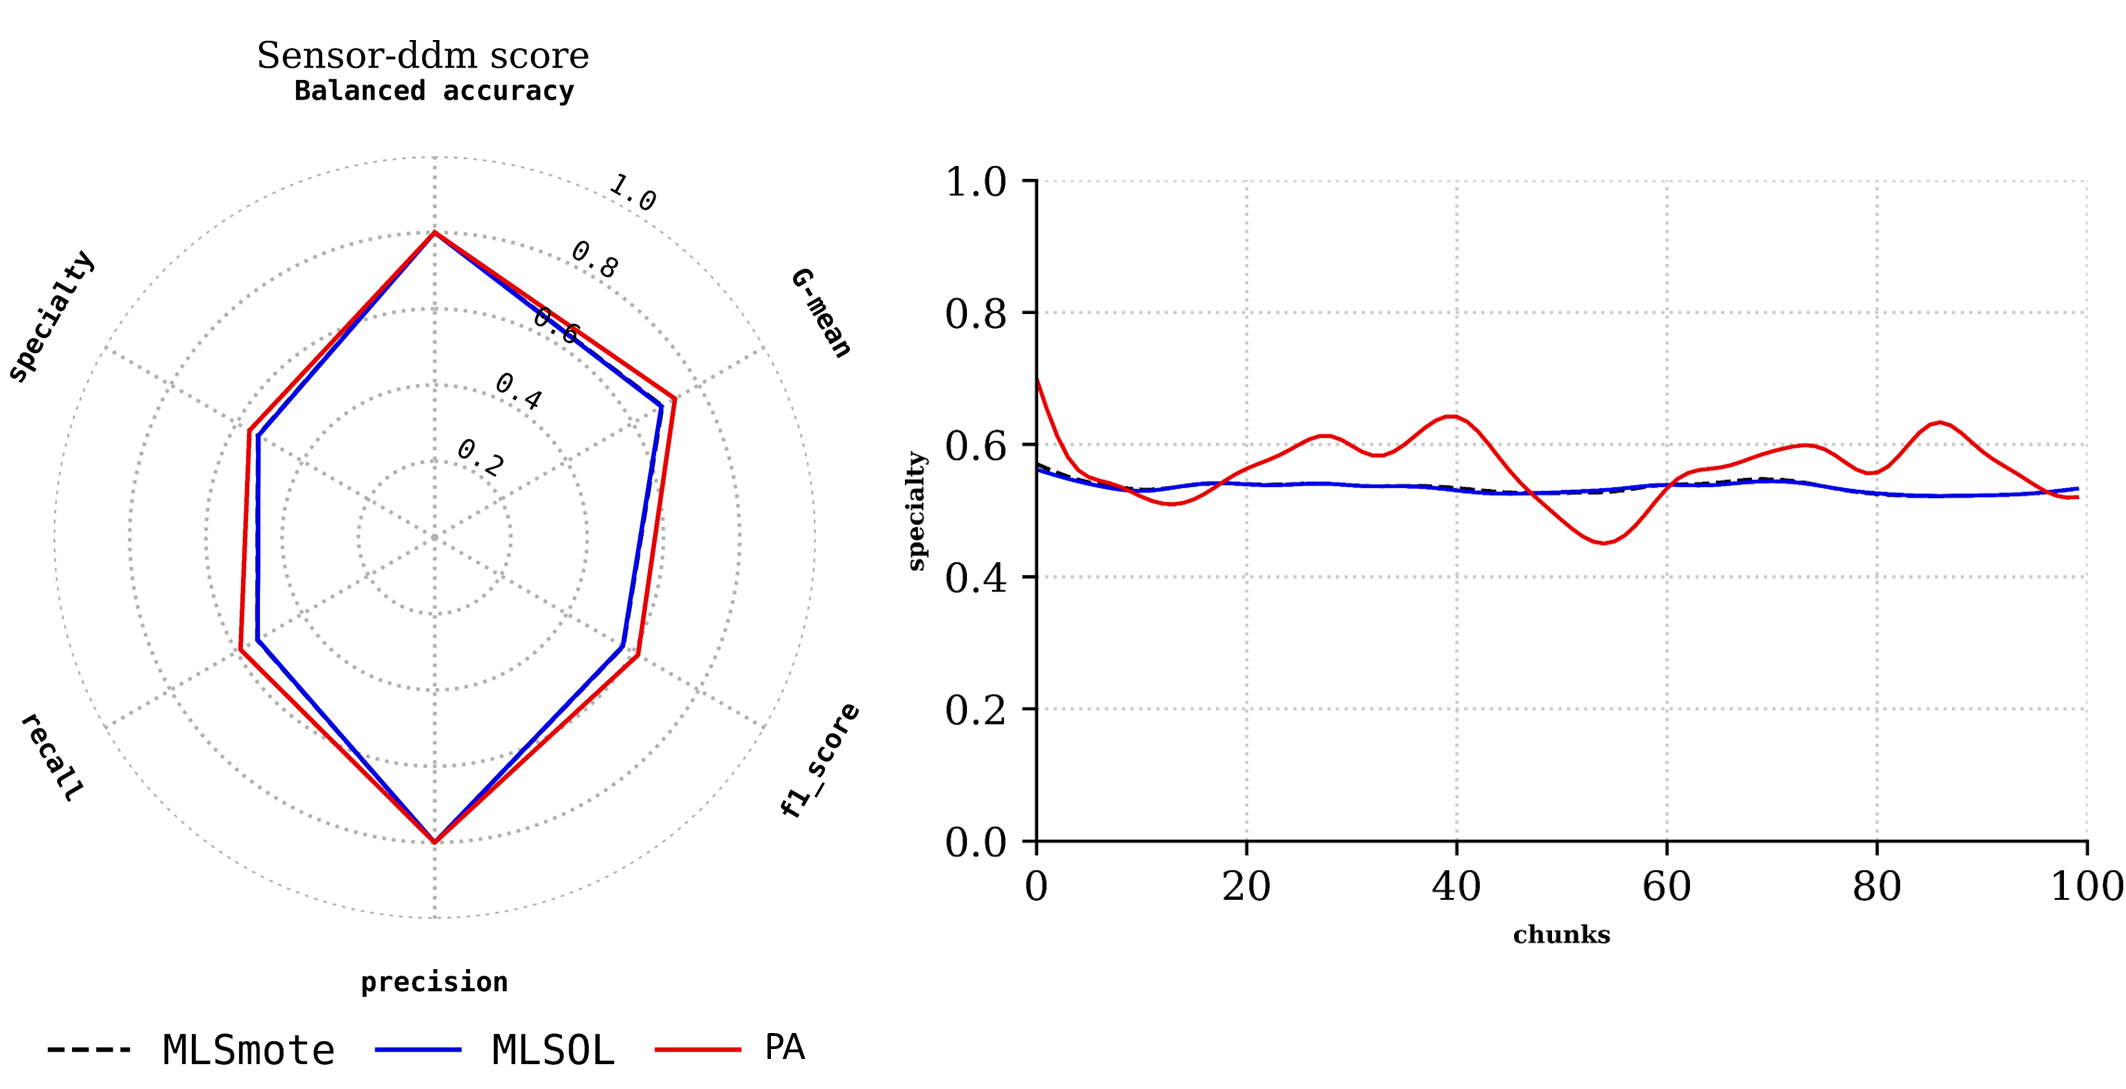
\includegraphics[width=1\linewidth]{4_Imbalanced/figures/exp_4.png}
  \caption{Performance of the Proposed Approach (PA), MLSMOTE, and MLSOL techniques on the Sensor real application stream using the DDM concept drift detector.}
	\label{fig:4_first_proposal_result_exp_4}
\end{figure}


\subsubsection{Results on the Synthetic Stream}
The results of applying the same methods on the synthetic data stream using ADWIN as the drift detector are presented in Fig. \ref{fig:4_first_proposal_result_exp_5}. The radar diagram indicates metric values ranging from 0.6 to 0.8, suggesting that the synthetic stream is prone to frequent drifts. While MLSOL exhibited the highest precision, MLSOTE exhibited the lowest values. Conversely, PA performed well in other metrics, and MLSMOTE demonstrated the least favorable values. Upon examining the line diagram in Fig. \ref{fig:4_first_proposal_result_exp_5}, it becomes evident that during the initial ten chunks, the PA's performance might be suboptimal because of the limited number of classifiers in the pool. However, after the first ten chunks, the performance improved significantly with the inclusion of more classifiers. In the same diagram, PA consistently achieves the highest performance across all chunks, whereas MLSOL maintains satisfactory performance, and MLSMOTE exhibits lower performance throughout. In Fig. \ref{fig:4_first_proposal_result_exp_6}, using the same synthetic data stream but with the DDM as the drift detector, the radar plot metrics produce similar results to the previous experiment. However, the line diagram emphasizes the same outcomes as those in the previous experiment. Nevertheless, MLSOL and MLSMOTE achieved lower values than the previous experiment. These findings confirmed ADWIN's superiority of ADWIN over DDM when applied to synthetic data streams. These results highlight the versatility and robustness of the algorithm, demonstrating its effectiveness in handling concept drift across diverse datasets, including the challenging synthetic dataset, Covertype dataset, and Sensor dataset, regardless of whether ADWIN or DDM is used as the concept drift detector.

\begin{figure}[!ht]
	\centering
	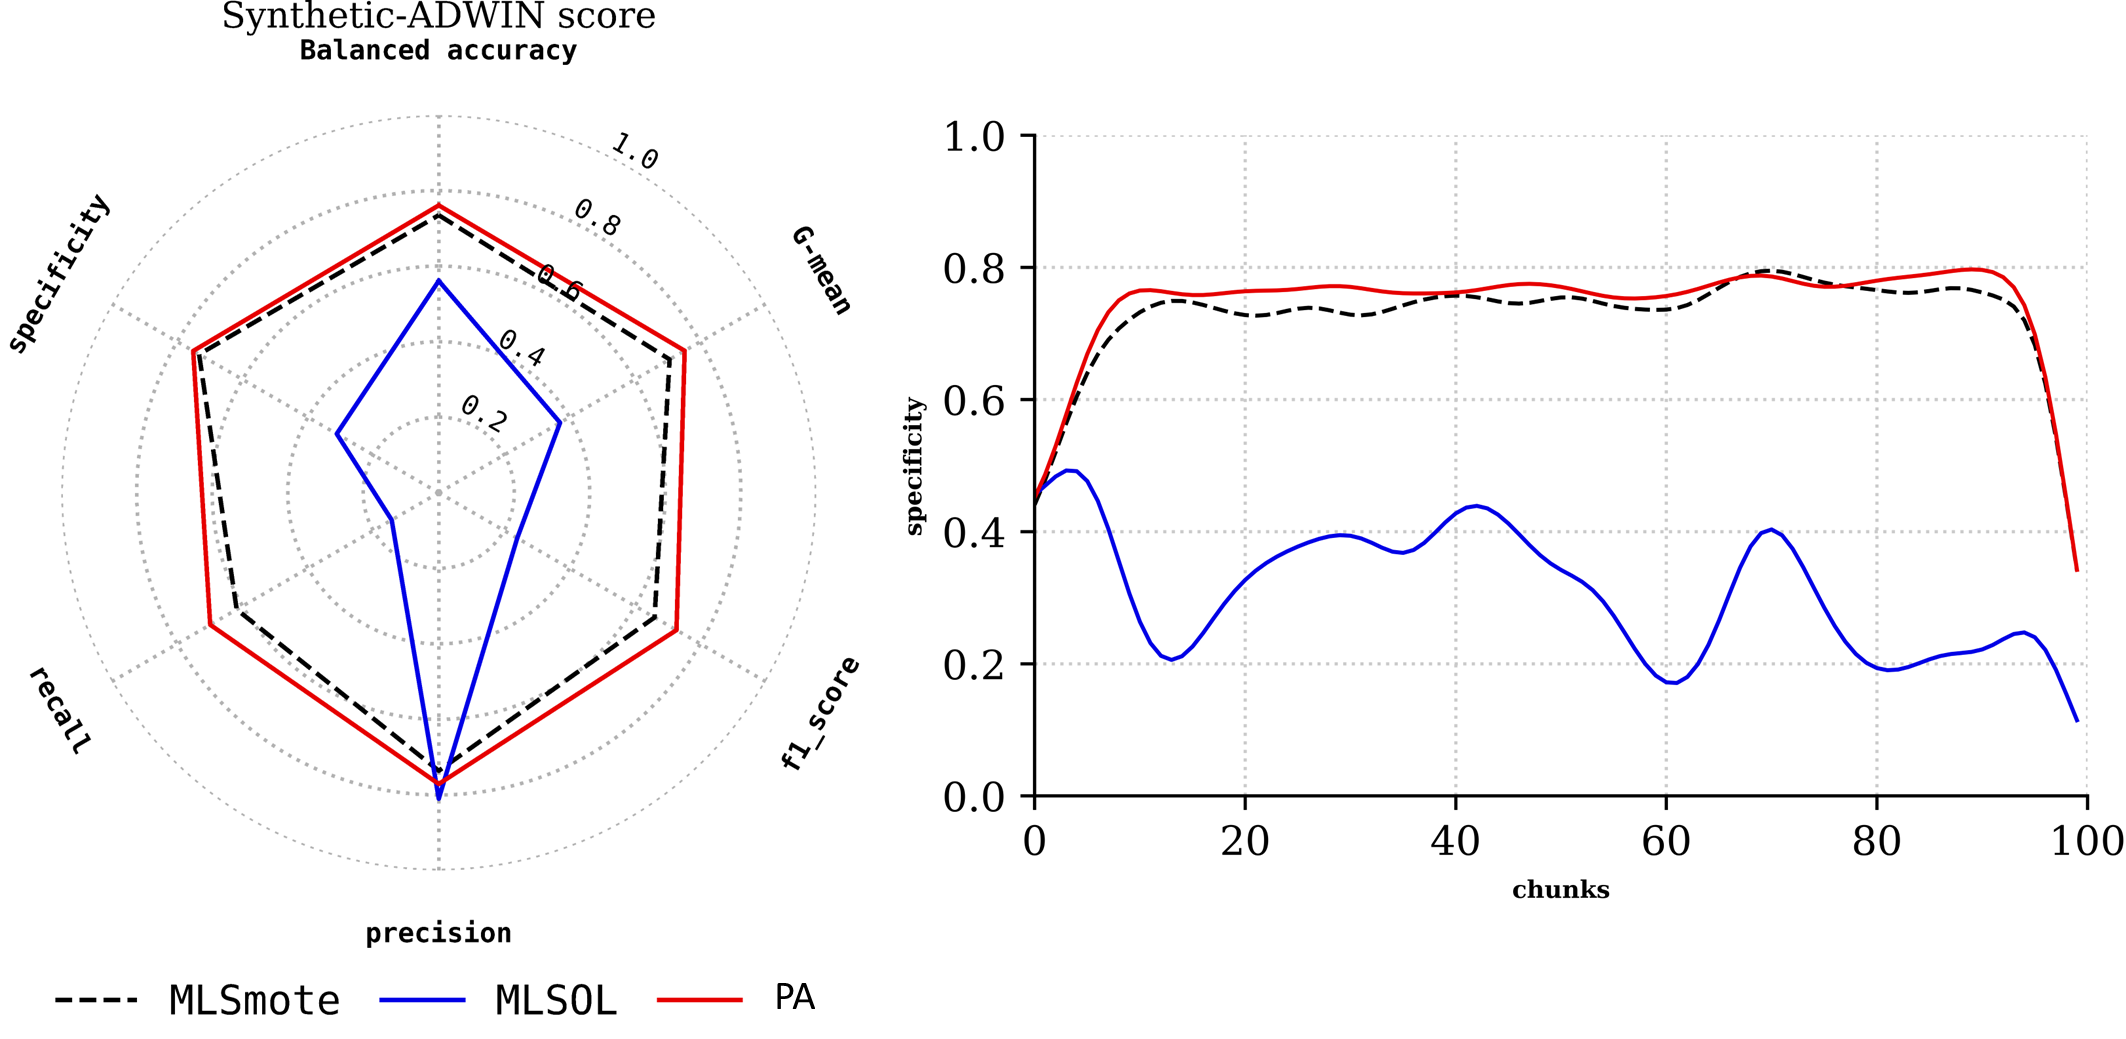
\includegraphics[width=1\linewidth]{4_Imbalanced/figures/exp_5.png}
  \caption{Performance of the Proposed Approach (PA), MLSMOTE, and MLSOL techniques on the Synthetic stream using the ADWIN concept drift detector.}
	\label{fig:4_first_proposal_result_exp_5}
\end{figure}

\begin{figure}[!ht]
	\centering
	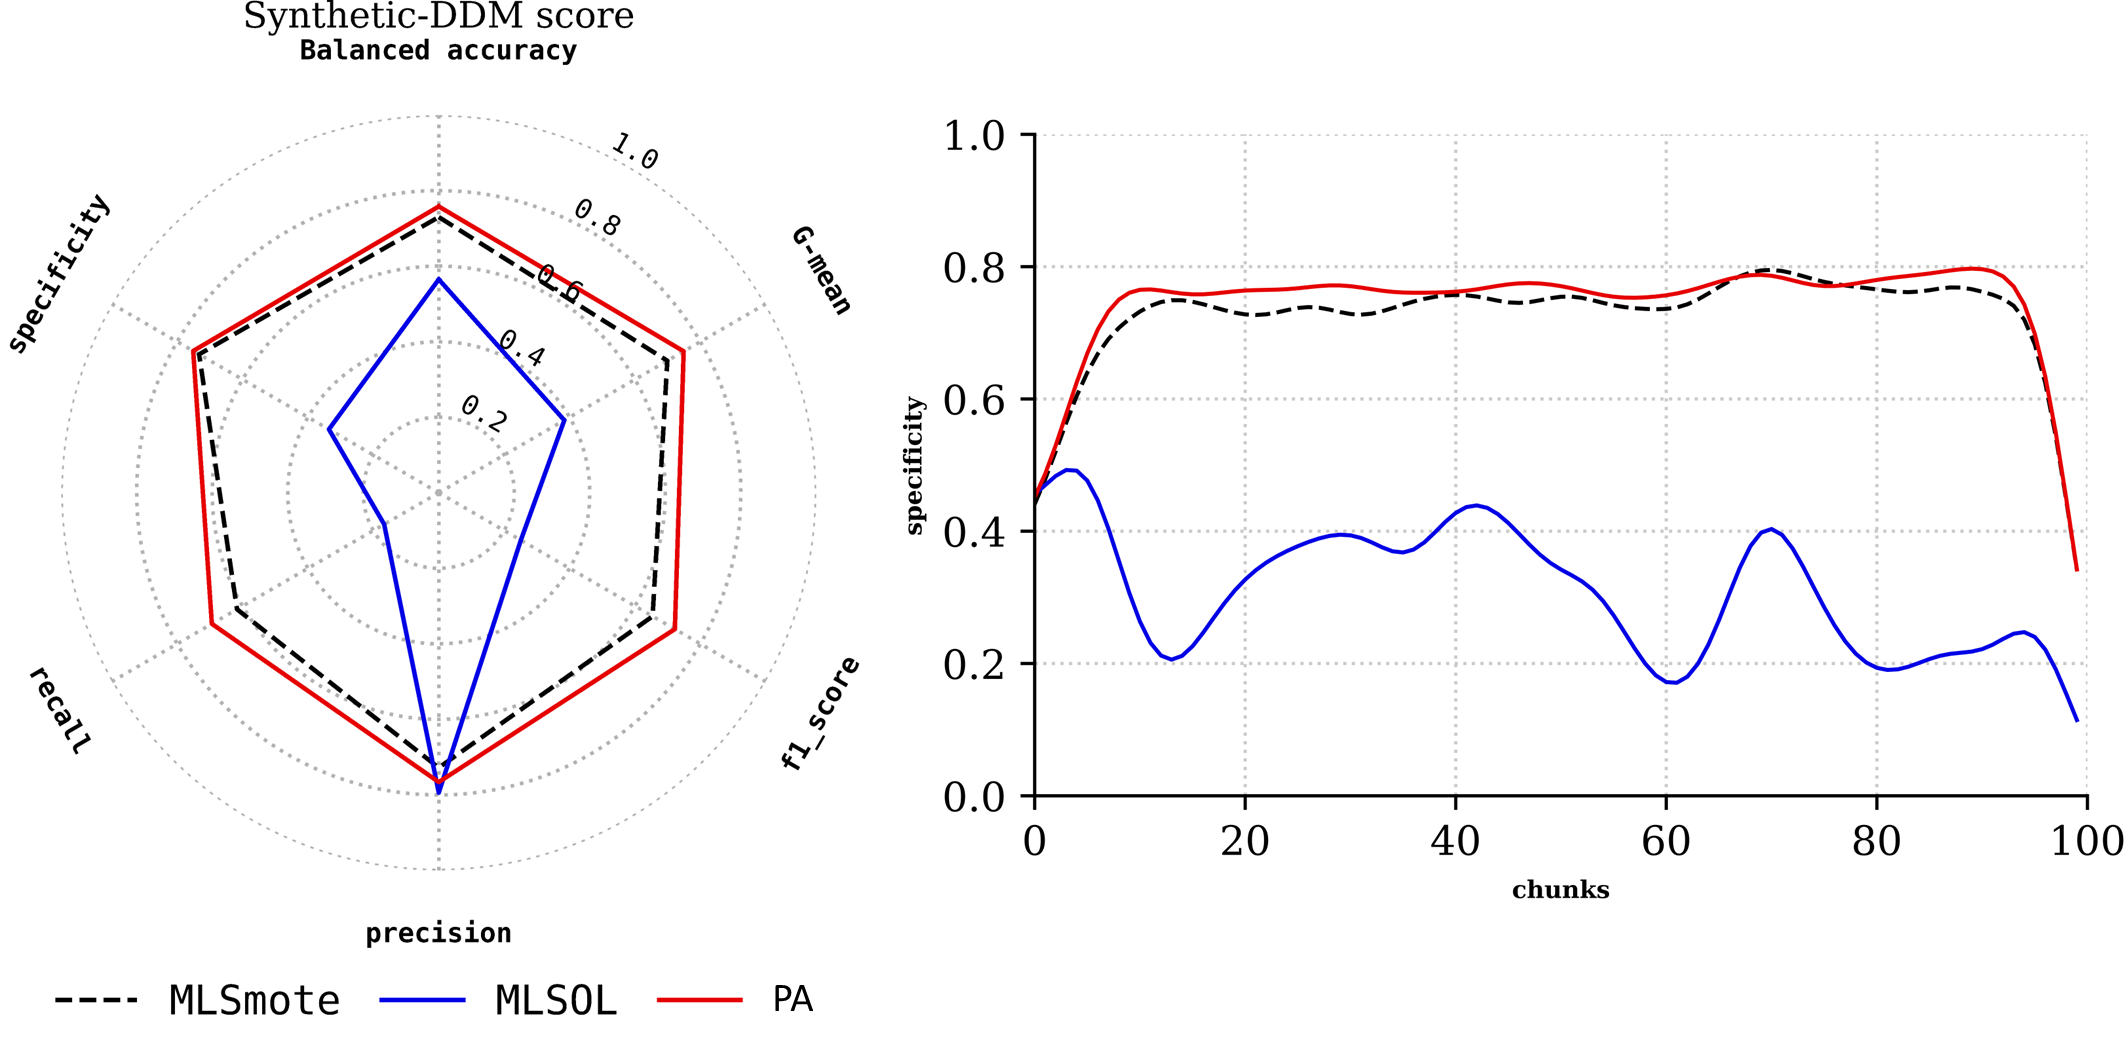
\includegraphics[width=1\linewidth]{4_Imbalanced/figures/exp_6.png}
  \caption{Performance of the Proposed Approach (PA), MLSMOTE, and MLSOL techniques on the Synthetic stream using the DDM concept drift detector.}
	\label{fig:4_first_proposal_result_exp_6}
\end{figure}


\subsection{Analysis of Class Overlap Factor between Proposed Approach (PA), MLSMOTE, and MLSOL Techniques.}
In our experimental study, we aimed to identify the critical factors that influence the selection of an optimal approach for minority classes in imbalanced drifted streams. These factors include various aspects, such as dataset characteristics, the choice of concept drift detectors, and the effectiveness of the algorithm in handling class overlap. To compare the overlapping class behavior of our proposed approach (PA) with MLSMOTE and MLSOL, we systematically designed experiments organized into groups of ten chunks. The results were visualized in bar diagrams, contrasting PA with other methods (MLSMOTE and MLSOL). Figures \ref{fig:4_first_proposal_result_exp_7, fig:4_first_proposal_result_exp_8, fig:4_first_proposal_result_exp_9} present ten groups, each with three bars representing MLSOTE, MLSOL, and PA, respectively. Each bar visually represents overlapped samples for ten chunks of several data streams, considering distinct concept drift detectors, specifically ADWIN and DDM.
Fig. \ref{fig:4_first_proposal_result_exp_7} shows two diagrams for the ADWIN and DDM detectors. In the ADWIN diagram, the third bar group (chunks 20-30) lacks overlapping samples because this chunk range does not have drifts, and no synthetic samples are generated for the training step. The sixth and tenth groups have the highest overlapped samples because these groups experience many drifts, leading to the generation of several samples and, consequently, the data indicates that MLSMOTE displays the highest number of overlapping samples across all groups, while PA exhibits very few, except for the last group (90-100), which has a small number of overlapping samples. However, the DDM diagram has more overlapping samples than the ADWIN diagram because the DDM detector detects fewer drifts than ADWIN. Specifically, the last value on the Y-axis of the ADWIN diagram is 3,000 samples, while the last value on the Y-axis of the DDM diagram is 2,000 samples. Fig. \ref{fig:4_first_proposal_result_exp_8} and Fig. \ref{fig:4_first_proposal_result_exp_9} display the overlapping samples of the three methods on the Sensor and synthetic data streams, respectively. In Fig. \ref{fig:4_first_proposal_result_exp_8}, the ADWIN diagram demonstrates fewer overlapped samples than in Fig. \ref{fig:4_first_proposal_result_exp_8}, indicating a lower number of drifts in the Sensor stream. The overall diagram indicates that our proposed approach achieves fewer overlapped samples than MLSOL and MLSMOTE, with MLSMOTE having the highest number of overlapped samples. In the DDM diagram of Fig. 10, the number of overlapped samples is lower than in Fig. \ref{fig:4_first_proposal_result_exp_7}, with our proposed approach consistently achieving the lowest number of overlapped samples across most group bars.
In Fig. \ref{fig:4_first_proposal_result_exp_9}, the ADWIN and DDM diagrams exhibit the greatest number of overlapped samples compared to the earlier figures. This suggests that the synthetic stream underwent frequent drifts and was more susceptible to noise. Consequently, the last value on the Y-axis in both the ADWIN and DDM diagrams was recorded for 7,000 samples. Our proposed approach consistently achieves the lowest number of overlapped samples, whereas MLSMOTE consistently attains the highest number of overlapped samples across most group bars in both the ADWIN and DDM diagrams. In conclusion, our thorough examination of overlapping class instances across MLSMOTE, MLSOL, and our proposed approach consistently reveals minimal overlapped samples compared to other methods, regardless of whether DDM or ADWIN is employed as drift detectors

\begin{figure}[!ht]
	\centering
	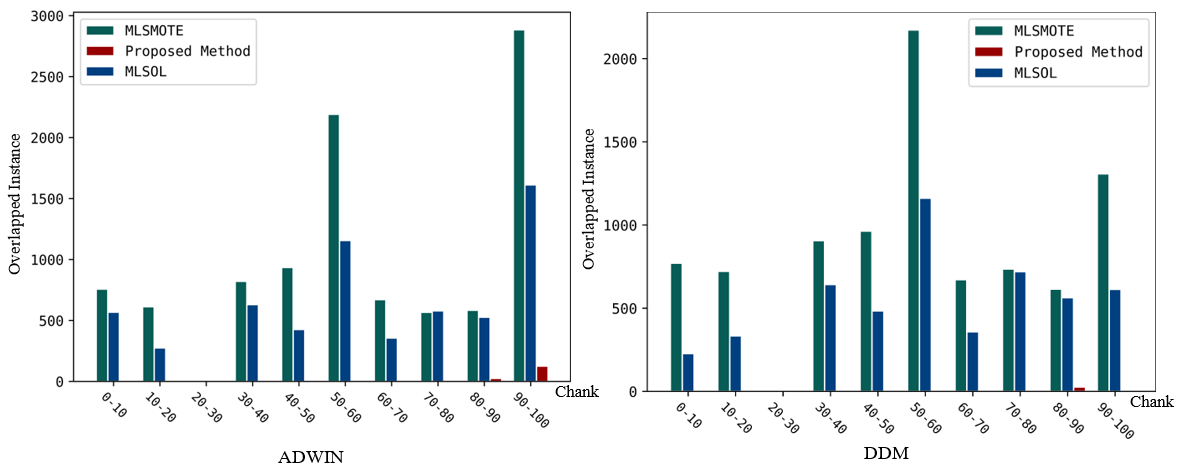
\includegraphics[width=1\linewidth]{4_Imbalanced/figures/exp_7.png}
  \caption{Overlapping generated points of the Proposed Approach (PA), MLSMOTE, and MLSOL techniques on the Covertype benchmark stream.}
	\label{fig:4_first_proposal_result_exp_7}
\end{figure}

\begin{figure}[!ht]
	\centering
	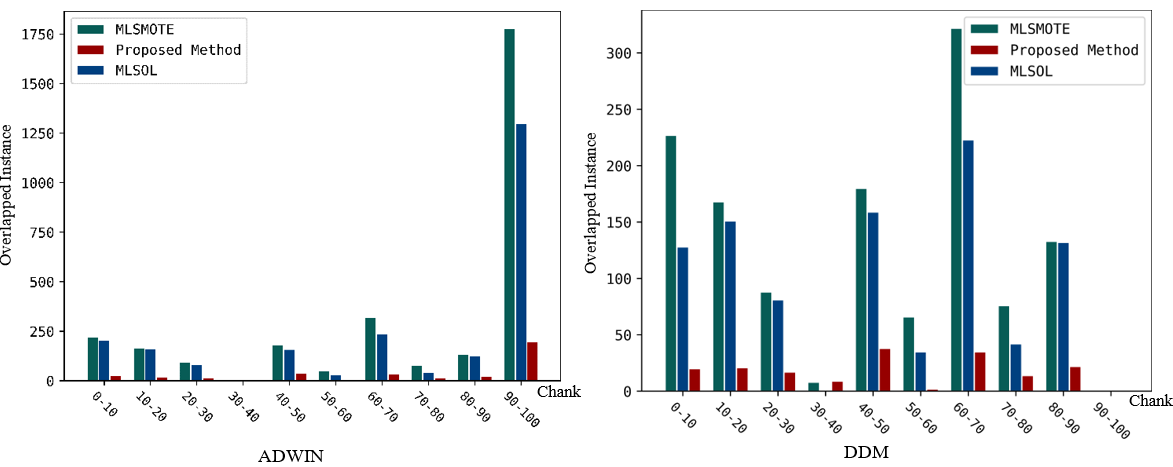
\includegraphics[width=1\linewidth]{4_Imbalanced/figures/exp_8.png}
  \caption{Overlapping generated points of the Proposed Approach (PA), MLSMOTE, and MLSOL techniques on the Sensor real application stream.}
	\label{fig:4_first_proposal_result_exp_8}
\end{figure}

\begin{figure}[!ht]
	\centering
	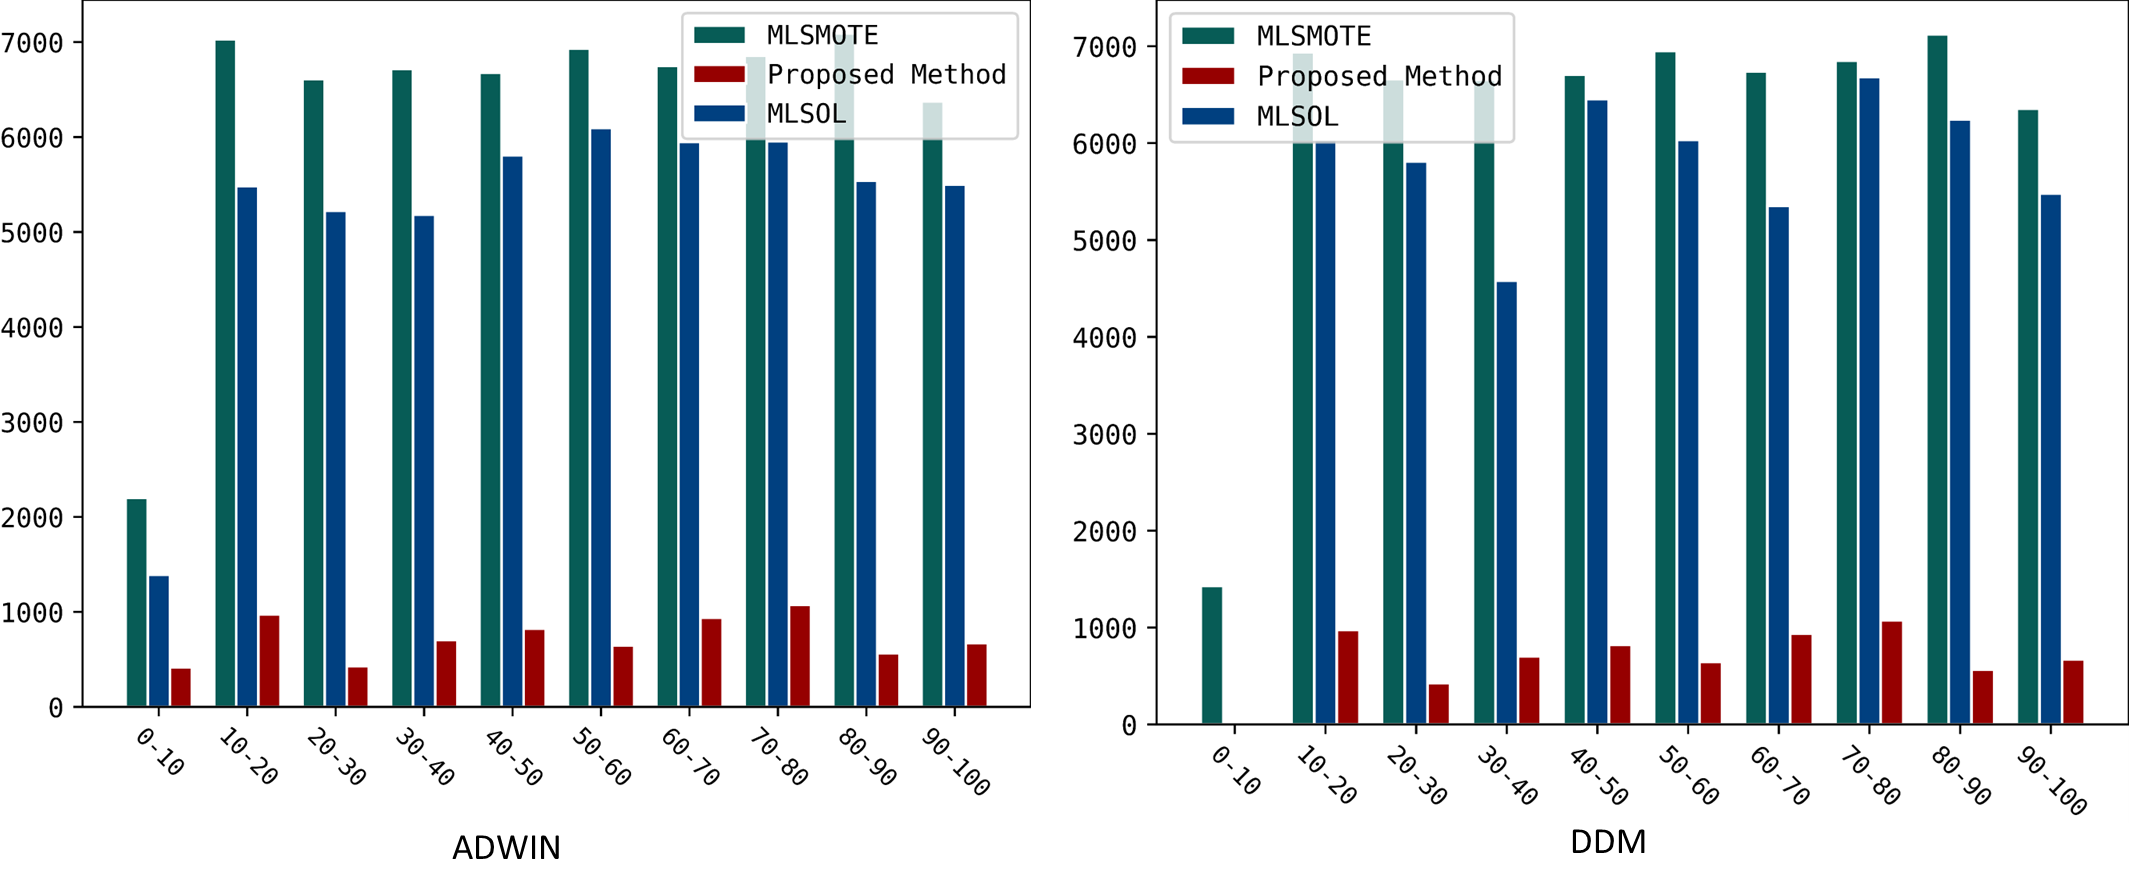
\includegraphics[width=1\linewidth]{4_Imbalanced/figures/exp_9.png}
  \caption{Overlapping generated instances of the Proposed Approach (PA), MLSMOTE, and MLSOL techniques on the synthetic stream.}
	\label{fig:4_first_proposal_result_exp_9}
\end{figure}

\subsection{Analyzing Runtime Factor Between the Proposed Approach, MLSMOTE, and MLSOL Techniques}
The results of our experiments indicate that the choice of the best algorithm for multiclass imbalanced streams depends on various factors, including dataset characteristics, the concept drift detector used, the presence of an overlapping class problem, and the algorithm's runtime demands. To investigate the runtimes of MLSMOTE, MLSOL, and our proposed approach, we conducted experiments, as shown in Table \ref{tab:4_first_proposal_result_table_2}. Our findings reveal that our proposed approach is highly efficient, regardless of whether ADWIN or DDM is used as the concept drift detector. Specifically, when ADWIN was used, the proposed approach algorithm took 8344 s to train and predict the Covertype stream for ensemble classifiers, whereas it took 8019 s when using the DDM detector. In contrast, MLSMOTE and MLSOL require more time for the same task. Notably, our proposed approach maintains efficiency, even when using the DDM concept detector. Additionally, our proposed approach demonstrates shorter processing times in the Sensor stream and synthetic data compared with other methods. Consistently, the DDM detector achieved less time across all experiments owing to its lower detection of drifts compared to the ADWIN detector. This is because there are fewer instances that trigger training for pool classifiers when using the DDM. The bold highlighting in Table \ref{tab:4_first_proposal_result_table_2} further emphasizes the efficiency of our proposed approach with both the ADWIN and DDM detectors across all dataset streams. Because our proposal generates fewer overlapped samples, leading to an overall decrease in the running time.

\begin{table}[h!]
  \centering
  \resizebox{\textwidth}{!}{
  \begin{tabular}{|l|l|c|c|c|}
  \hline
  \textbf{Stream} & \textbf{Concept Drift Detector} & \textbf{MLSMSOTE} & \textbf{MLSOL} & \textbf{PA} \\ \hline
  \multirow{2}{*}{Benchmark} & ADWIN & 9559 & 8655 & \textbf{8344} \\ \cline{2-5} 
   & DDM & 8388 & 8031 & \textbf{8019} \\ \hline
  \multirow{2}{*}{Real Application} & ADWIN & 1291 & 1310 & \textbf{1102} \\ \cline{2-5} 
   & DDM & 585 & 607 & \textbf{521} \\ \hline
  \multirow{2}{*}{Synthetic} & ADWIN & 12870 & 4866 & \textbf{4834} \\ \cline{2-5} 
   & DDM & 12397 & 4958 & \textbf{4687} \\ \hline
  \end{tabular}
  }
  \caption{Runtime of MLSMOTE, MLSOL, and the Proposed Approach (PA).}
  \label{tab:4_first_proposal_result_table_2}
  \end{table}

\subsection{Analyzing Non-parametric Tests between the Proposed Approach, MLSMOTE, and MLSOL Techniques}
We conducted a thorough series of statistical analyses encompassing 12 comparisons across three diverse datasets, three methods, and two drift detectors. These analyses were rigorously evaluated using a non-parametric test, specifically the Kruskal-Wallis test. The results of this test were striking, revealing substantial variations in the G-mean measurements across most experiments. Importantly, these differences were not due to random chance \cite{yamada2013change}. Upon closer examination of the assessments for the three methods, PA, MLSMOTE, and MLSOTE, as detailed in Table \ref{tab:4_first_proposal_result_table_3}, we found compelling evidence supporting the acceptance of the null hypothesis (H0).
This implies that the expected and observed data exhibited statistically significant disparities. H0 is rejected when significant differences are not observed and H0 is accepted if the P-value falls below the critical value. Underlining the significance of our analysis, the Kruskal-Wallis test was conducted with a 95\% confidence level, and the P-value was rounded to the first three digits after the decimal point. Nevertheless, it is important to note that a similarity in the performances of the methods emerged in the third and fourth experiments, resulting in the rejection of H0. This similarity can be attributed to the fact that the DDM detected fewer drifts in these experiments.


\begin{table}[h!]
  \centering
  \resizebox{\textwidth}{!}{
  \begin{tabular}{|c|c|c|c|c|c|}
  \hline
  \multirow{2}{*}{Dataset} & \multirow{2}{*}{Drift detector} & \multirow{2}{*}{Comparison} & \multirow{2}{*}{P-value} & \multirow{2}{*}{Critical value} & \multirow{2}{*}{H0} \\ 
                           &                                 &                             &                           &                                 &  \\
  \hline
  \multirow{4}{*}{Covertype stream} & \multirow{2}{*}{ADWIN} & PA - MLSSMOTE & 0.001 & 0.05 & Accept \\ \cline{3-6}
                                    &                        & PA - MLSOL    & 0.014 & 0.05 & Accept \\ \cline{2-6}
                                    & \multirow{2}{*}{DDM}   & PA - MLSSMOTE & 0.361 & 0.05 & Rejected \\ \cline{3-6}
                                    &                        & PA - MLSOL    & 0.401 & 0.05 & Rejected \\ 
  \hline
  \multirow{4}{*}{Sensor stream} & \multirow{2}{*}{ADWIN} & PA - MLSSMOTE & 0.001 & 0.05 & Accept \\ \cline{3-6}
                                 &                        & PA - MLSOL    & 0.001 & 0.05 & Accept \\ \cline{2-6}
                                 & \multirow{2}{*}{DDM}   & PA - MLSSMOTE & 0.001 & 0.05 & Accept \\ \cline{3-6}
                                 &                        & PA - MLSOL    & 0.001 & 0.05 & Accept \\ 
  \hline
  \multirow{4}{*}{Synthetic stream} & \multirow{2}{*}{ADWIN} & PA - MLSSMOTE & 0.001 & 0.05 & Accept \\ \cline{3-6}
                                    &                        & PA - MLSOL    & 0.001 & 0.05 & Accept \\ \cline{2-6}
                                    & \multirow{2}{*}{DDM}   & PA - MLSSMOTE & 0.001 & 0.05 & Accept \\ \cline{3-6}
                                    &                        & PA - MLSOL    & 0.001 & 0.05 & Accept \\ 
  \hline
  \end{tabular}
  }
  \caption{Kruskal-Wallis test results for MLSMOTE, MLSOL, and PA.}

  \label{tab:4_first_proposal_result_table_3}
  \end{table}

%%%%%%%%%%%%%%%%%%%%%%%%%%%%%%%%%%%%%%%%%%%%%%%
%
%   Conclusions
%
%%%%%%%%%%%%%%%%%%%%%%%%%%%%%%%%%%%%%%%%%%%%%%%

%%%%%%%%%%%%%%%%%%%%%%%% Here it is needed to re-frame the conclusions

\section{Conclusion and Future Works}
\label{sec:4_8_Conclusions}

Our study in this chapter presents a comprehensive methodology designed to facilitate incremental learning in drifted streams, with a particular focus on addressing the challenges associated with imbalanced data streams including minority and overlapping classes. The proposed methodology integrates our proposed oversampling method, concept drift detection strategies, and Dynamic Ensemble Selection (DES) to select the most suitable ensemble classifier. Extensive experimentation across various datasets, including benchmark datasets, real application streams, and synthetic data, validated the effectiveness of this contribution. The critical role of the concept drift detector in our approach lies in its capacity to promptly detect concept drifts, allowing our methodology to adapt by training new base classifiers to maintain relevance and performance in real-time scenarios. Oversampling techniques were utilized to mitigate the minority class problem, and the KNN algorithm was employed to prevent the generation of overlapped class instances. The DES technique was utilized to intelligently select the best base classifiers to ensure optimal performance. Our evaluation approach employs various performance measures, showcasing its proficiency in addressing multiclass imbalanced stream problems, particularly its exceptional performance in classifying data streams with evolving class distributions. In addition to its performance and performance, our approach has several advantages, including adaptability, efficiency, and scalability. Dynamic model updates driven by incoming data instances enable continuous adaptation to changing data distributions, thereby ensuring reliability and relevance in real-time scenarios. However, it is essential to recognize the specific limitations of the proposed approach. One limitation is the extended time required to generate nonoverlapping performance instances. Moreover, the efficacy of our contribution depends on the performance of the MLSMOTE and MLSOL techniques. Consequently, future research efforts should be directed toward enhancing our contributions. Potential avenues for improvement include the development of advanced oversampling techniques to avoid generating overlapping synthetic instances. Additionally, meta-learning methods have been explored to calculate imbalanced multiclass ratios and minority classes.


%emerging
% this file is called up by thesis.tex
% content in this file will be fed into the main document

 
% this file is called up by thesis.tex
% content in this file will be fed into the main document

%: ----------------------- introduction file header -----------------------


\begin{savequote}[50mm]
  You cannot teach a man anything; you can only help him discover it in himself.
  \qauthor{Galileo}
  % The beginning is the most important part of the work.
  % \qauthor{Plato}
  \end{savequote}
  
  
  \chapter{Dynamic Classification Ensembles for Handling Imbalanced
  Multiclass Drifted Data Streams}
  \label{chapter:5_emerging}
  
  In various real-world applications, data streams have introduced new challenges to learning algorithms. Data streams are continuous with high volumes of data arriving rapidly and dynamically. This data deluge poses unprecedented challenges for learning algorithms because they must adapt to the dynamic nature of the data environment \cite{yang2021concept}\cite{dong2019multistream}\cite{shan2018online}. Among the various research areas in machine learning, incremental learning under data Streams with Emerging New Classes (SENC) has garnered considerable attention because of its practical relevance and unique challenges \cite{da2014learning}\cite{mu2017streaming}\cite{zhu2020semi}. SENC refers to a scenario in which new classes that were not present during the initial training of a learning model emerged in the data stream. This poses a significant challenge for traditional learning approaches that are typically designed to handle fixed or predefined class distributions. The ability to effectively recognize and adapt to these novel classes in real-time is crucial for maintaining accurate and up-to-date models. Furthermore, the inherent limitations of data streams, such as limited memory and storage constraints, impose additional complexities in the learning process. Learning algorithms must operate efficiently within these resource constraints to ensure real-time processing and to avoid overwhelming computational overhead.
  To address the challenges presented by data streams containing emerging new classes, dynamic ensemble selection (DES) \cite{cruz2017meta}\cite{jackowski2014improved}\cite{kuncheva2000clustering}. Dynamic ensemble selection involves utilizing multiple classifiers in machine learning to make collective predictions or classifications of data. Dynamic ensemble selection is distinguished by its ability to dynamically adapt the ensemble based on the characteristics of the data. Instead of relying on a fixed ensemble of classifiers, dynamic ensemble selection continuously assesses the performance of individual classifiers and selects the subset that demonstrates the highest competence for the current data. This adaptability enables the ensemble to enhance its performance over time by incorporating the most suitable classifiers for prevailing data conditions. Furthermore, if a classifier becomes ineffective owing to concept drift or the emergence of new classes, it can be excluded from the ensemble to prevent it from negatively affecting the overall performance.
   Adaptive Windowing (ADWIN) is another widely employed method to address concept drift. Concept drift refers to the phenomenon in which the statistical properties of data change over time, leading to a decline in the learning algorithm performance \cite{gama2004learning}\cite{adams2023explainable}\cite{madkour2023historical}. ADWIN continuously monitors incoming data and detects changes or drifts in data distribution. It achieves this by maintaining sliding windows of variable sizes and monitoring statistical measures such as the mean or variance within these windows. Upon detecting a significant change or drift, the ADWIN triggers an update in the ensemble or classifier configuration. This update may involve retraining the classifiers with new data or incorporating new classifiers that are better suited to the updated data distribution. By adapting the ensemble to changing data conditions, ADWIN ensures that the classifier system remains accurate and up-to-date even in the presence of concept drift or the emergence of new classes. The primary objective of utilizing these approaches, such as dynamic ensemble selection and ADWIN, is to establish a flexible and effective classification system that is capable of handling data streams containing emerging new classes. By dynamically adjusting the ensemble based on the data characteristics and detecting and adapting to concept drift, these approaches enable the system to maintain accurate predictions over time. Adaptability and responsiveness are crucial for addressing the unique challenges posed by the dynamic nature of data streams and the emergence of new classes within them.  
  This research proposes efficient algorithms for classifying data streams in real-time scenarios, focusing on addressing the challenges posed by emerging new classes in data distributions. 
  The subsequent sections of this paper adhere to a well-structured organization. Section 2 presents a comprehensive review of the relevant literature encompassing concept drift, dynamic classifier ensembles, and emergency class detection methods. Section 3 introduces the proposed framework, providing intricate explanations of its constituents, including dynamic classifier ensembles, concept drift handling, and emergency class identification, and the adaptive proposed method of the emerging pool size. Section 4 outlines the experimental setup and presents the results, providing details regarding the employed datasets, evaluation metrics, and procedures. Finally, in Section 5, we offer concluding remarks, summarizing the key findings, discussing their implications, and proposing potential avenues for future research.
  
  
  The remainder of this chapter is organized as follows: In Section \ref{sec:5_2_motivation}, we present the motivations and the contributions. The proposed framework and combination via SI algorithms are discussed in detail in Section \ref{sec:5_4_proposed}. The  experimental results and the discussion are presented in Sections \ref{sec:5_5_Expsetup} and \ref{sec:5_7_Discussion}, respectively. Finally, the conclusions of this study and future research are discussed in Section \ref{sec:5_8_Conclusions}. 
  
  
  \section{Motivations and Contributions} \label{sec:5_2_motivation}
  We aim to develop novel algorithms that can effectively handle the emergence of new classes issue in nonstationary data streams, achieve high classification accuracy, and minimize computational complexity. The key contributions of this study are outlined as follows:
   
  \begin{enumerate}[nosep]
    \item Our first contribution involves utilizing the ADWIN, DES, and K-means techniques in combination with the ensemble stratified bagging technique to detect and adapt to emerging new classes. This approach allows us to dynamically update the classification model to accommodate an evolving data environment.
   \item The second contribution is the introduction of an adaptive method to adapt the emerging pool size depend on the stream distribution.
    \end{enumerate} 
   
     
  
  
 
   



\section{Proposed Methodology}\label{sec:5_first_proposed_approach}

In this section, we present the primary phases of our study, which consist of three distinct steps designed to address the challenges of handling emerging new classes in drifted streams. Our proposed approach aims to develop a robust framework capable of tackling these complex challenges through a comprehensive, three-step methodology.
\begin{itemize}
	\item \textbf{Emerging New Classes:} Our study addresses the widespread issue of emerging new classes in drifted streams using well-known techniques, including concept drift detection and K-means clustering.
	\item \textbf{Drifted Streams: } To handle changes in the data distribution, our approach integrates a concept drift detector that dynamically identifies shifts, allowing the model to promptly adapt its classifiers to maintain effectiveness.
	\item \textbf{Classifier Performance:} The final phase identifies unknown classes in drifted streams, creating new classifiers for emerging classes to improve the model's ability to classify new instances accurately.
\end{itemize}

\subsection{THE PROPOSED APPROACH Flow}

Our proposed approach is designed with three distinct phases that work together to improve its performance in managing multiclass imbalanced and drifting data streams. 
\begin{itemize}
	\item \textbf{DES Phase (dynamic ensemble selection phase):} The first phase, known as the dynamic ensemble selection (DES) phase, is responsible for selecting the most appropriate classifier for the incoming data. This ensures that the selected classifier is well-suited for the current data chunk.
	\item \textbf{Drift detector phase:} The second phase of our approach is the drift detector phase, which operates in real-time to continuously monitor the data stream. Its primary function is to identify any signs of concept drift, which indicates shifts in the underlying data distribution over time.
	\item \textbf{Emerging New Class Identifier Phase:} The final phase of our approach is the synthetic data generator phase, which is dedicated to generating synthetic data for the minority classes. This step is crucial for addressing class imbalance by producing additional samples for underrepresented classes, thereby significantly enhancing the model's ability to accurately classify instances from minority classes.
\end{itemize}

As depicted in Fig. \ref{fig:5_first_proposal_step_1}, the DES phase retrieves the current data chunk and applies the DES technique to select the best classifiers for the chunk (black box of Fig.  \ref{fig:5_first_proposal_step_1}). These classifiers are used in the second phase to predict class labels, while drift detectors like ADWIN or DDM monitor for concept drift. If a drift is detected (highlighted by the red rectangle), the chunk is forwarded to the third phase, where new classes are identified (see Fig.  \ref{fig:5_first_proposal_step_2}). The overall approach is implemented in Algorithm  \ref{alg:5_1}, which takes a data stream and a DES Pool threshold as inputs. Key components include training the initial ensemble (Lines 4-6), using DES to select the best classifier for the current chunk (Line 8), detecting drifted chunks (Line 10), creating new classifiers for emerging classes (Line 12), and removing the worst classifier if the DES Pool threshold is exceeded (Lines 14-16).


\subsection{Emerging New Classes Phase Details}

In this section we present the Emerging new classes phase details. As shown in Fig.2, The emerging phase contains two primary steps: 
\begin{itemize}
	\item 	\textbf{Emerging new classes identifier:} The emerging class detection step plays a crucial role in the proposed approach (the black rectangle of Fiq.2) by utilize the K-means technique to clustering the drifted chunk into a set of clusters. And identifying new emerging classes by evaluating the distances between instances and their nearest class centroid. This process involves comparing the distance between an instance and the nearest class centroid with the maximum distance between class centroids ($d_c$), as described in Eq. \ref{eq:5_first_proposal_1} and Eq. \ref{eq:5_first_proposal_2}, where ED represents the Euclidean Distance method and ci, cj denotes the centroids of the current classes. If the calculated distance ($d_x$) exceeds this threshold ($d_c$), this indicates the presence of a new emerging class, denoted by EC in Eq. \ref{eq:5_first_proposal_3}; otherwise, it is $P_\text{DES}$ (prediction class of the new instance).
	\item \textbf{Adaptive the Emerging classes pool size:} This critical step adapts the pool size based on the emergence rate of new classes and drift distribution, using statistical measures like standard deviation, first derivative, and average historical drift updates.
	The Emerging New Classes phase is implemented in Algorithm  \ref{alg:5_2}, which utilizes drifted instances and current changes as inputs. Key steps include applying K-means (Line 1), calculating cosine similarity between centroids (Line 2), determining the maximum centroid distance (Line 3), setting the adaptive pool threshold (Lines 4-7), using KNN to find the nearest neighbor (Line 9), storing instances in the emerging pool if the distance exceeds the threshold (Lines 11-12), and creating a new classifier if the pool size surpasses the adaptive limit (Lines 14-17). A simulated scenario is illustrated in Figures 3 and 4. In Fig. \ref{fig:5_scenario1}(a), the drifted chunk is divided into three clusters using the K-means algorithm. Fig. \ref{fig:5_scenario1}(b) shows the calculation of the maximum distance between cluster centroids, which serves as a threshold for identifying new classes. The procedure for classifying instances is as follows: when a drifted instance is detected, it is considered a new class if the distance between the instance and its nearest centroid exceeds the maximum inter-centroid distance (Fig. \ref{fig:5_scenario2} a). If the distance is within the threshold, the instance is classified as a known class (Fig. \ref{fig:5_scenario2} b).
\end{itemize}

\begin{figure}[!ht]
	\centering
	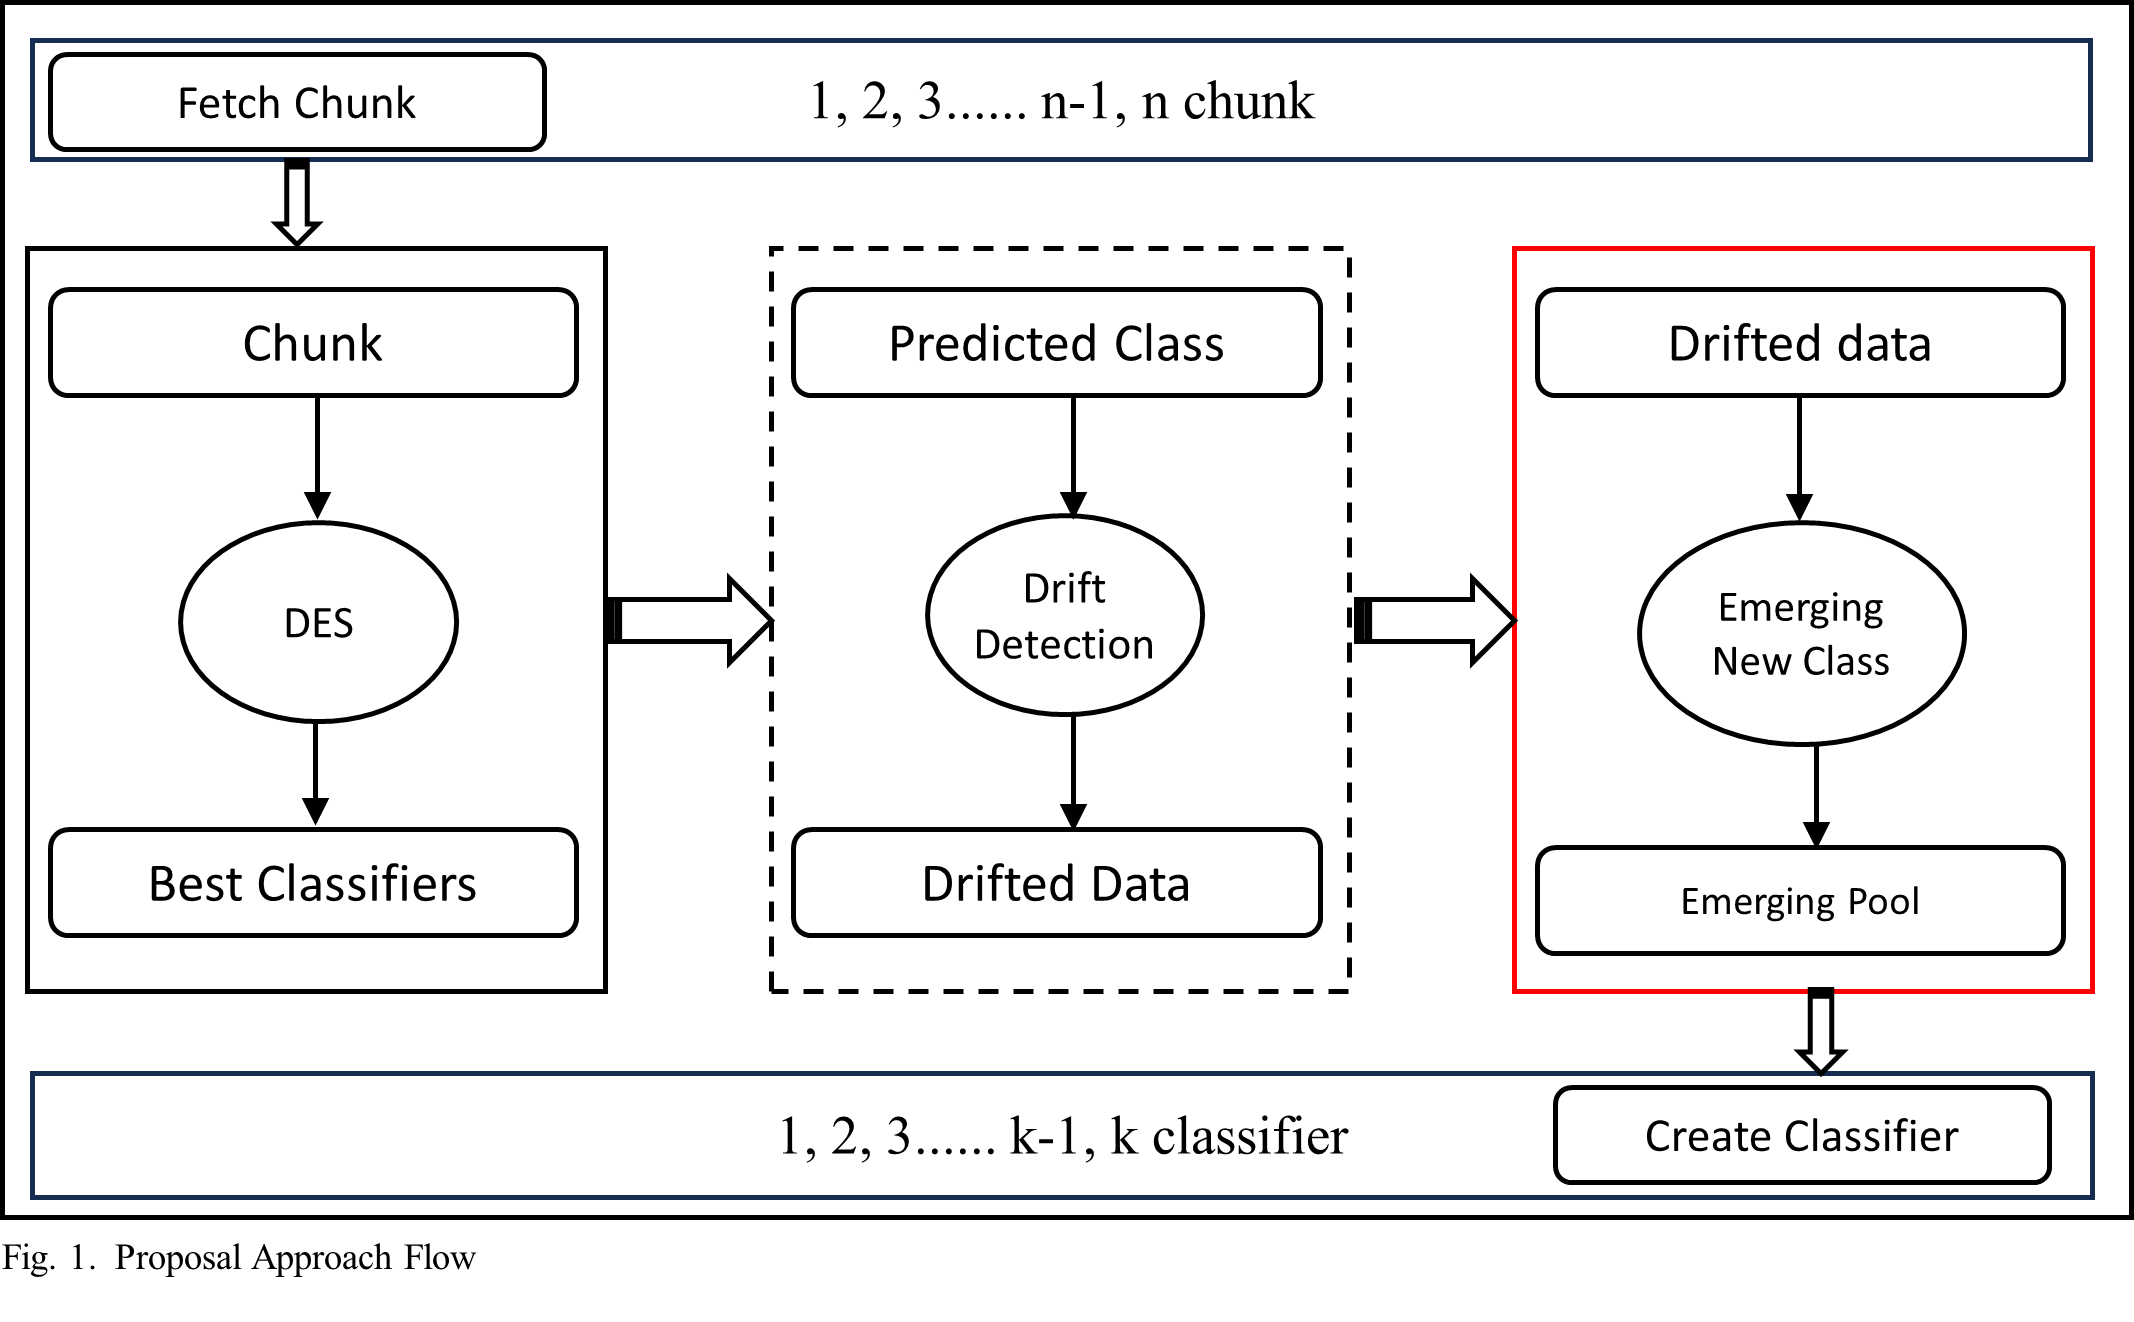
\includegraphics[width=1\linewidth]{5_Emerging/figures/algorithm1.png}
	\caption{Proposed Approch Flow}
	\label{fig:5_first_proposal_step_1}
\end{figure}
\begin{figure}[!ht]
	\centering
	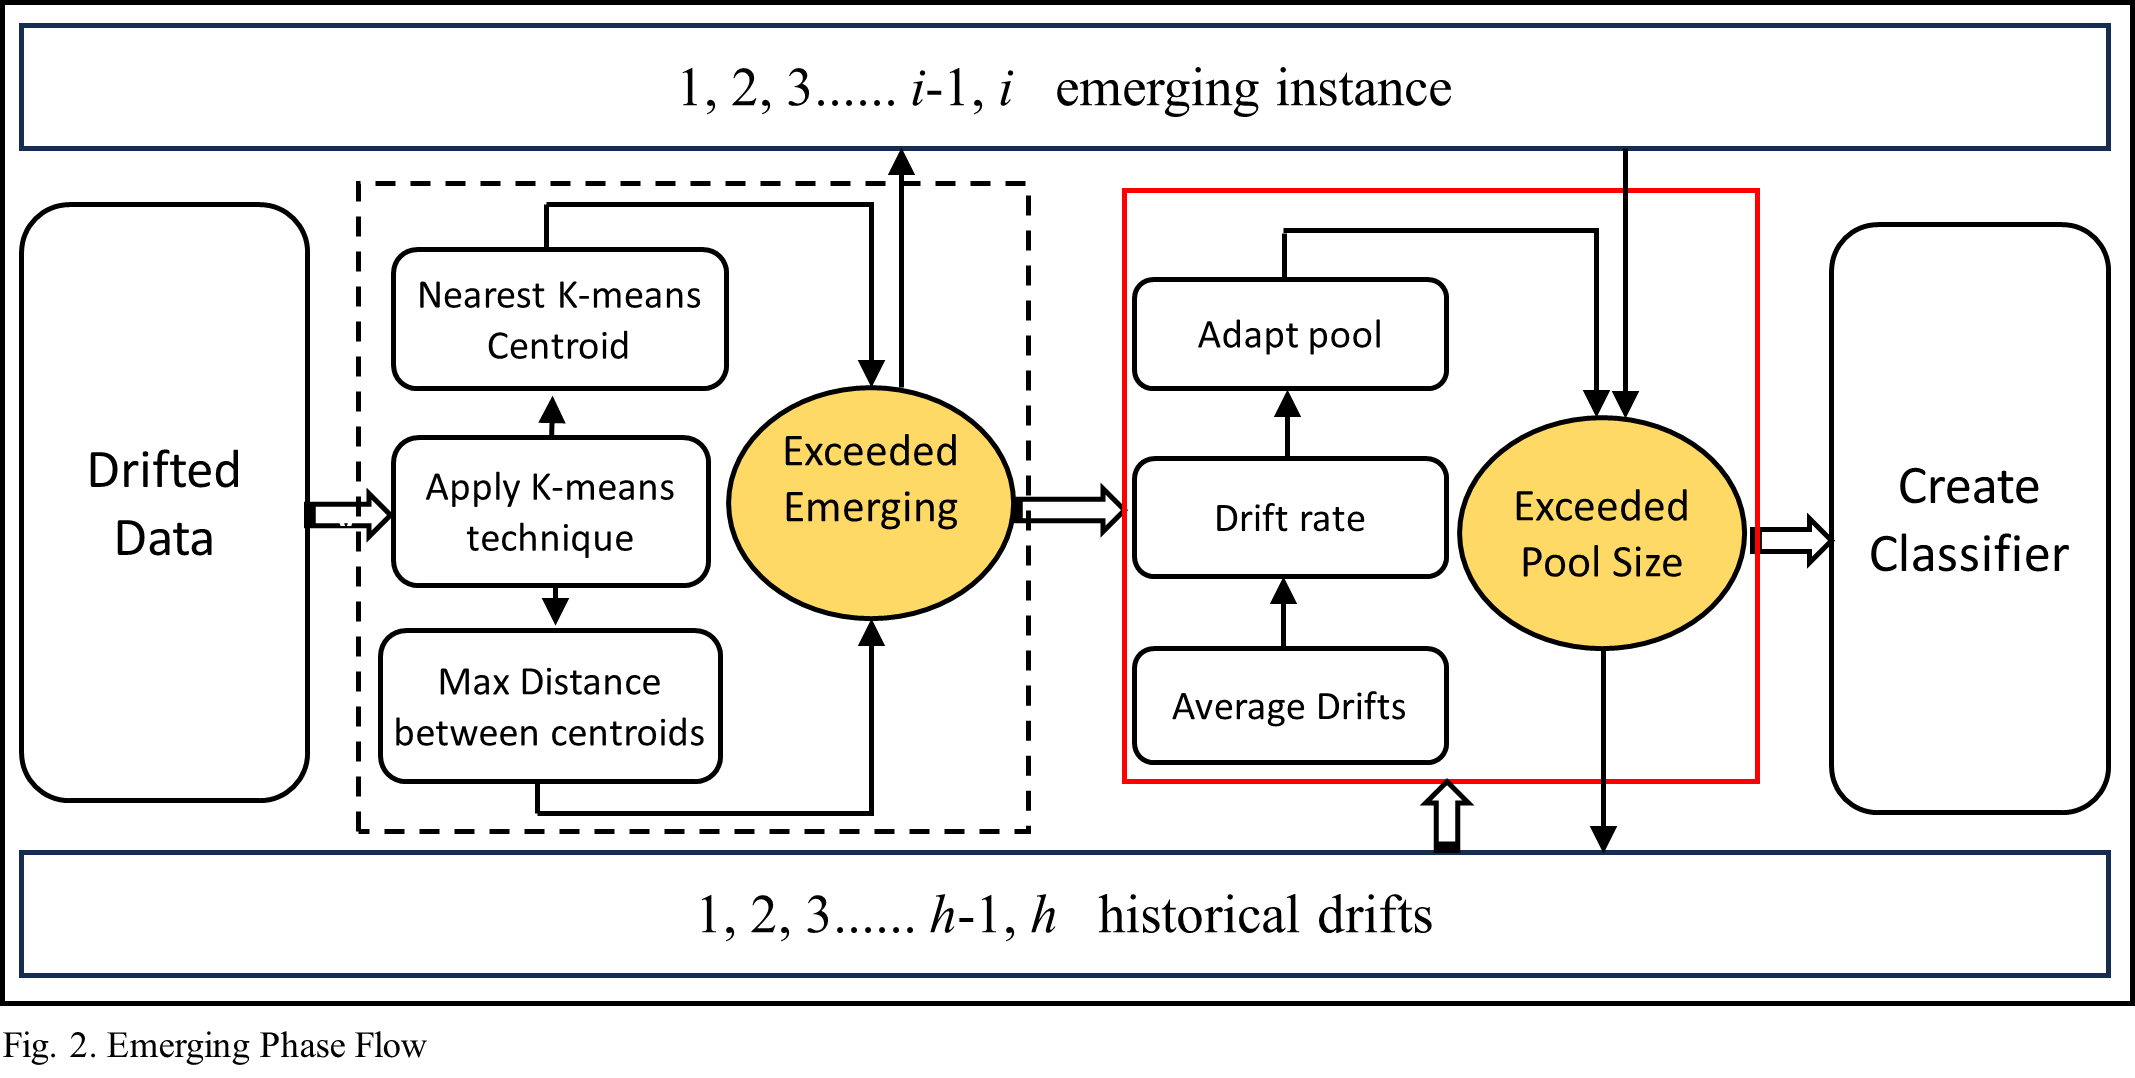
\includegraphics[width=1\linewidth]{5_Emerging/figures/algorithm2.png}
	\caption{Emerging Phase Flow}
	\label{fig:5_first_proposal_step_2}
\end{figure}
\begin{figure}[!ht]
	\begin{center}
	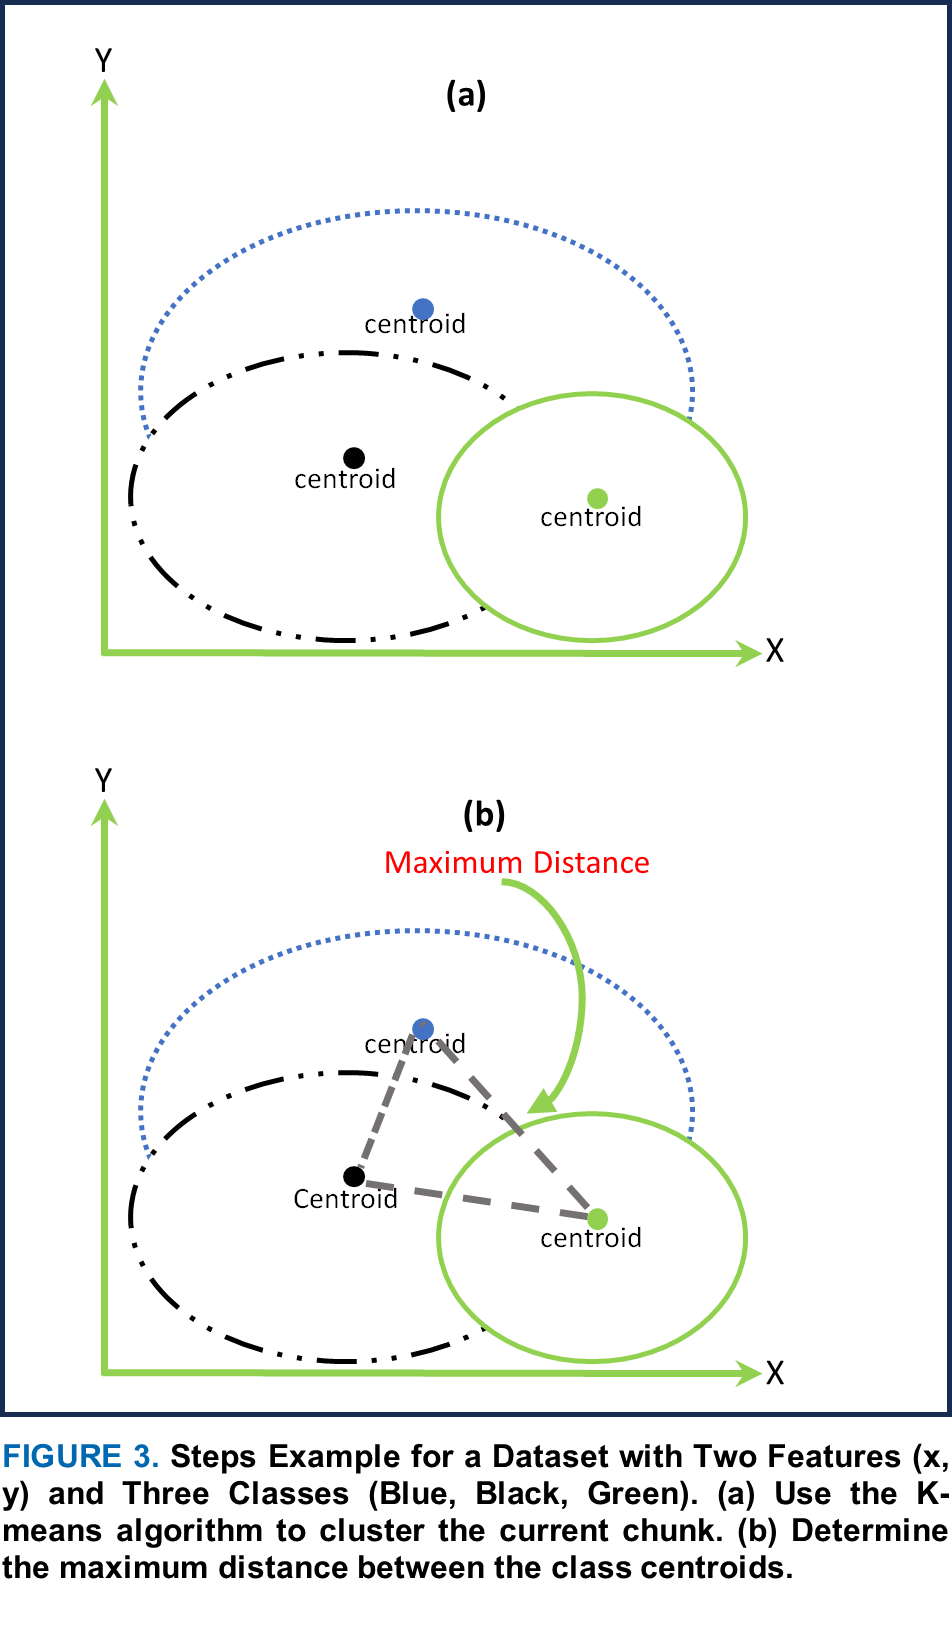
\includegraphics[width=0.48\linewidth]{5_Emerging/figures/scenario1.png}
	\caption{Proposed Approch Flow}
	\label{fig:5_scenario1}
	\includegraphics[width=0.48\linewidth]{5_Emerging/figures/senario2.png}
	\caption{Emerging Phase Flow}
	\label{fig:5_scenario2}
\end{center}

\end{figure}

\begin{equation}
	\label{eq:5_first_proposal_1}
    d_c = \arg\max_d \sum_{i=1}^{i} \sum_{j=i+1}^{i} d = ED(c_i, c_j)
\end{equation}

\begin{equation}
	\label{eq:5_first_proposal_2}
	d_x = \arg\min_i \sum_{i=1}^{i} ED(x, c_i)
\end{equation}

\begin{equation}
	\label{eq:5_first_proposal_3}
    \begin{cases}
		EC & \text{if } d_x > d_c \\
		P_{DES} & \text{otherwise}
	\end{cases}
\end{equation}

\begin{algorithm}[H]
	\caption{Proposed Framework Algorithm for Imbalanced Multi-Class Drifted Data Streams}
	\label{alg:5_1}
	\KwIn{data stream, maximum classifiers pool size $\kappa$}
	% \Parameter{current chunk $a$, synthetic data $b$, classifiers pool $\Psi$, drifted pool $\psi$, classes frequency $\Omega$, best frequency $\omega$, minority classes $\mu$}
	\KwOut{Prediction $P$}
	\BlankLine
	$\psi, \Psi, \Omega, \mu \gets \emptyset$\;
	$\omega \gets 0$\;
	\For{stream have chunk}{
		\eIf{$a$ is the First chunk}{
			$k \gets$ \texttt{trainingNewClassifier}($a$)\;
			$P \gets$ \texttt{getPrediction}($a, k$)\;
		}{
			$k \gets$ \texttt{DES}($a, \Psi$)\;
			$P \gets$ \texttt{getPrediction}($a, k$)\;
			$\psi \gets$ \texttt{conceptDriftDetector}($P$)\;
			\If{$\psi > 0$}{
				$\Omega \gets$ get classes frequency according to Eq.1\;
				$\omega \gets$ best frequency according to Eq.2\;
				$\mu \gets$ get minority classes according to Eq.3\;
				$b \gets$ utilize $a$ and $\mu$ to get the synthetic data according to Algorithm 2\;
				trainingData $\gets a + b$\;
				$k \gets$ \texttt{trainingNewClassifier}(trainingData)\;
				$\Psi \gets \Psi + k$\;
				\If{$\Psi > \kappa$}{
					\texttt{removeWorstClassifier}($\Omega$)\;
				}
			}
			$P \gets$ \texttt{getPrediction}($a, k$)\;
		}
	}
	\Return{$P$}
	\end{algorithm}
	
	\vspace{1cm}
	
	\begin{algorithm}[H]
		\caption{Synthetic data generator}
		\label{alg:5_2}
		\KwIn{Minority classes $\mu$, current chunk $a$, sample size $\eta$, historical chunks $h$}
		\KwOut{Generated data $b$}
		$b \gets \emptyset$\;
		$f \gets \text{MLSMSOTE}$\;
		$knn \gets \text{kNearestNeighbor}(a)$\;
		$chunk \gets \text{similarChunk}(a, h)$\;
		$f \gets \text{similarChunkOverSamplingMethod}(chunk)$\;
		\If{$f = \text{MLSMSOTE}$}{
			$f \gets \text{MLSOL}$\;
		}
		\Else{
			$f \gets \text{MLSMSOTE}$\;
		}
		\While{$|b| < \eta$}{
			$p \gets \text{generateSyntheticPoint}(\mu, f)$\;
			$similarPointsClass \gets \text{KNN.getKneighbor}(b)$\;
			\If{$similarPointsClass = \mu$}{
				$b \gets b \cup \{p\}$\;
			}
		}
		\Return $b$\;
		\end{algorithm}


%transfer
\chapter{Dynamic Classification Ensembles for Handling Imbalanced
Multiclass Drifted Data Streams}
\label{chapter:6_transfer_learning}

Transfer learning plays a pivotal role in addressing the intricate challenges posed by dynamic data streams and inherent concept drifts. Transfer learning aims to enhance a model's learning performance within a target domain by leveraging the knowledge gleaned from the source domains \cite{pan2009survey}\cite{wang2019characterizing}. This research domain focuses extensively on addressing target tasks that grapple with limited or unlabeled data, with a dual emphasis on amplifying positive knowledge transfer and alleviating negative knowledge transfer \cite{wang2019characterizing}. To facilitate the transfer of valuable knowledge, researchers have developed diverse techniques, including methodologies aimed at reducing the domain gap, such as instance re-weighting \cite{zadrozny2004learning}\cite{cortes2008sample}\cite{pan2010domain} and feature matching \cite{sun2016return}\cite{pan2010domain}. Conversely, strategies for mitigating negative knowledge transfer often involve down weighting irrelevant data sources \cite{wang2019characterizing}.
Although a substantial body of transfer learning research has focused on static environments, where data in each domain are assumed to conform to the same distribution, real-world scenarios, including financial data analysis, energy demand prediction, and climate data analysis, often involve dynamic environments. Within these dynamic contexts, the concept drift problem \cite{li2015learning}\cite{cao2019learning} emerges as data distributions evolve over time. Dynamic environment transfer learning requires continuous adaptation to concept drift and adaptive utilization of valuable knowledge from source domains within each distinct environment. These new challenges in transfer learning, particularly within dynamic environments, represent a profound departure from traditional transfer learning paradigms that do not inherently address concept drift and the dynamic nature of evolving data.
To overcome these challenges, Dynamic Ensemble Selection (DES) \cite{cruz2017meta}\cite{jackowski2014improved}\cite{kuncheva2000clustering}, ADWIN, and Streaming Ensemble Algorithm (SEA) have become prominent in the scientific literature \cite{gama2004learning}\cite{adams2023explainable}\cite{madkour2023historical} Dynamic ensemble selection employs multiple classifiers within the realm of machine learning to make collective predictions or classifications, and leverage data characteristics. Its key feature is its dynamic adaptability, as it continuously evaluates the performance of individual classifiers and selects a subset that demonstrates the highest competence within the prevailing data conditions. This adaptability empowers the ensemble to progressively enhance its performance by incorporating best-fitting classifiers for the existing data context. Moreover, ineffective classifiers can be excluded from the ensemble in scenarios marked by concept drift, thereby protecting the overall performance from detrimental effects.
Adaptive Windowing (ADWIN) is another widely used method designed to address the challenges of concept drift \cite{madkour2023historical}. Concept drift refers to the phenomenon in which the statistical properties of data change over time, leading to a decline in the learning algorithm performance. ADWIN monitors incoming data by maintaining sliding windows of variable sizes and evaluating statistical attributes, such as the mean or variance within these windows. Upon detecting substantial shifts or drifts, the ADWIN initiates adjustments to the ensemble or classifier configuration. These adjustments may involve retraining classifiers with fresh data, or incorporating new classifiers that are better suited to the updated data distribution. Additionally, the Streaming Ensemble Algorithm (SEA) is an integral component for addressing these dynamic challenges \cite{gama2004learning}\cite{adams2023explainable}\cite{madkour2023historical}. SEA is specifically designed to manage data streams and inherent concept drifts. This is achieved by adapting the ensemble of classifiers in real time as new data arrives. SEA's adaptability of SEA ensures that the ensemble remains robust and accurate even in the face of shifting data conditions and the emergence of new classes.
This study proposes efficient algorithms for classifying data streams in real-time scenarios, focusing on addressing the challenges posed by heterogeneous transfer learning in data distributions. The goal is to develop a novel algorithm (Heterogeneous Transfer Learning) that can effectively handle non-stationary data streams, achieve high classification accuracy, and minimize computational complexity. 
The subsequent sections of this paper adhere to a well-structured organization. Section 2 comprehensively reviews the relevant literature on concept drift and transfer learning. Section 3 introduces the proposed approach, providing intricate explanations of its constituents, including dynamic classifier ensembles, concept drift handling, and heterogeneous multisource transformation. Section 4 outlines the experimental setup and presents the results, providing details regarding the employed datasets, evaluation metrics, and procedures. Finally, in Section 5, we offer concluding remarks, summarizing the key findings, discussing their implications, and proposing potential avenues for future research.
\section{Motivations and Contributions} \label{sec:4_2_motivation}
This paper presents a novel contribution to real-time streaming scenarios by addressing the challenges of heterogeneous multisource streams, with key contributions that can be summarized as follows:
\begin{enumerate}[nosep]
  \item The primary innovation involves incorporating a concept drift detection method in conjunction with an ensemble classifier, enabling real-time adaptation and refinement of the proposed approach in response to transfer learning in non-stationary environments. This methodology ensures continuous evolution of the classification model in accordance with the changing data landscape.
  \item The second significant advancement is the introduction of a precise weighting method to assess the significance of each local classifier within the ultimate classifier.
 \item The third significant contribution is the development of an innovative approach that employs the eigenvector technique to facilitate the transfer of knowledge from heterogeneous source domains to the target domain.
  \end{enumerate} 
 
   


\section{Third Proposed Methodology}\label{sec:6_third_proposed_approach}

In this section, we introduce the Heterogeneous Transfer Learning (HTL) algorithm tailored for non-stationary environments. HTL adeptly assimilates knowledge from both heterogeneous and homogeneous sources, operating within the framework of data streams subject to concept drift. Leveraging an online learning inductive parameter transfer strategy, HTL achieves seamless knowledge transfer. We delineate the core components and workflow of the HTL algorithm. To address the challenges intrinsic to our approach, we focus on three key aspects:
\begin{itemize}
	\item \textbf{Heterogeneous sources:} Traditional transfer learning methods often assume homogeneity in the data distribution across source and target domains. However, in real-world scenarios, data sources may vary significantly in terms of feature space. HTL addresses this challenge by allowing knowledge transfer from sources with different dimensionalities. This means that the algorithm can effectively learn from diverse dimentionality sources, enabling a more comprehensive knowledge transfer process.
	\item \textbf{Drifted streams:} In dynamic environments, data distributions may change over time, leading to concept drift. This phenomenon poses a significant challenge for machine learning algorithms, as models trained on historical data may become obsolete as the underlying data distribution shifts. HTL incorporates a concept drift detector that continuously monitors the incoming data stream. Upon detecting a shift in the data distribution, the algorithm adapts its classifiers accordingly to ensure continued effectiveness in handling drifting streams. This dynamic adjustment mechanism allows HTL to maintain high performance even in the presence of concept drift.
	\item \textbf{Classifier performance:} Classifier performance is crucial for the overall effectiveness of the transfer learning process. HTL employs Dynamic Ensemble Selection (DES) to enhance classifier performance. DES creates a diverse ensemble of classifiers, each trained on different subsets of the data. When presented with a new data point, DES dynamically selects the most suitable classifiers from the ensemble based on its performance on similar chunk. This adaptive selection process ensures that the most appropriate classifier is chosen for each data point, leading to improved classification accuracy and robustness. By leveraging DES, HTL maximizes the utility of available classifiers, resulting in superior performance in non-stationary environments with heterogeneous data sources.
\end{itemize}

\subsection{HTL Overall Details}

The aim of this section is to harness knowledge from diverse dimensional multisource domain streams. Following a similar framework to CDTL \cite{yang2021concept}, this approach employs a class-wise and domain-weighted strategy. However, HTL enhances the weight function of CDTL in a class-wise manner, as demonstrated in Equation 1. This equation factors in both correct and incorrect predictions for each classifier class, with K representing the number of classifiers in the current chunk, C denoting the number of classes in the current chunk, and i indicating the current chunk. The components of HTL operate synergistically, as depicted in Fig. \ref{fig:6_alg1}, encompassing three phases:
\begin{itemize}
	\item \textbf{Dynamic ensemble selection phase (DES Phase):}: The primary objective DES phase is to identify the optimal classifier for incoming data. This is crucial for ensuring that the selected classifier effectively aligns with the unique characteristics of the current data segment.
	\item \textbf{Drift detector phase:} After the DES phase, our method advances to the drift detector phase, where it operates in real-time to continually monitor the data stream. This phase employs ADWIN and DDM techniques, which play a pivotal role in swiftly identifying any signs of concept drift. These techniques are designed to detect changes in the underlying data distribution over time, thus enabling the algorithm to adapt to evolving data patterns.
	\item \textbf{Feature scaling} The concluding phase of our approach is featuring scaling, operating in real-time to harmonize the diverse dimensionalities of the multisource streams with the target dimensionality. Leveraging the eigen vector technique, this phase facilitates the transformation of data into a unified dimensionality, essential for creating new classifiers tailored to the target and domain streams. By ensuring compatibility with the learning framework, this process enhances the algorithm's effectiveness in handling diverse dimensionality streams.
\end{itemize}
\subsection{Classifier Creation Details }

Fig. \ref{fig:6_alg2} provides a comprehensive overview of the classifier creation phase, a crucial component responsible for generating new classifiers based on the current chunk of the target domain, previous classifiers, and source domain classifiers. This phase offers several advantages and perform three tasks. \begin{itemize}
	\item \textbf{Source projection:} This step involves projecting the source domain classifiers onto the current chunk of the target domain. The projection likely employs the source weight function, as described in CDTL \cite{yang2021concept}, to assign a weight to each classifier based on its relevance to the current chunk of data. This weighting mechanism ensures that classifiers from the source domains contribute appropriately to the creation of the new classifier for the target domain.
	\item \textbf{Class-wise weights:} This block computes class-specific weights for each classifier using Equations \ref{eq:6_eq_1} and \ref{eq:6_eq_2} . The process involves analyzing the current chunk of the target stream (denoted as \emph{D}) and considering both correct and incorrect predictions made by each classifier where $prediction_i$ refers to the predicted class of the current instance and $c$ to the income class. These weights are crucial for determining the significance of individual classifiers across different classes. The equations facilitate the calculation of weights that reflect the classifiers' performance on specific classes, enabling the creation of a well-balanced ensemble classifier.
	\item \textbf{Classifier combination:} In this phase, the class-wise weights, along with the current chunk of data and the projected source domain classifiers, are combined to derive the final classifier. The combination process follows the details outlined in Eq. \ref{eq:6_eq_3} , where historical classifiers (denoted as \emph{H}), projected data classifiers (denoted as \emph{P}), and the classifier of the current chunk (denoted as \emph{K}) are integrated. This integration ensures that the resulting classifier incorporates contributions from both historical and projected data sources, leveraging the strengths of each to enhance predictive performance. The resulting classifier is then utilized to make predictions based on the data chunk, effectively leveraging the insights gleaned from both historical and current data sources.
\end{itemize}

\subsection{HTL Detailed Algorithm}

As illustrated in Algorithm \ref{alg:6_alg_1}, the HTL algorithm involves several stages, beginning with training a classifier for the target stream and proceeding through various steps related to heterogeneous multisource preprocessing, classifier weighting, concept drift detection, and classifier management to ensure the accuracy and adaptability of the final classifier. In this section, detailed explanations of each individual step within the HTL algorithm are provided.
\begin{itemize}
	\item \textbf{Converting heterogeneous multisource to homogeneous multisource:} In the initial step, the algorithm unifies the various data sources that might have different characteristics (heterogeneous multisource). This is achieved using eigenvectors and the feature count of the current chunk (line 7).
	\item \textbf{Training a new classifier for the first target chunk:} In line 8, the new classifier is trained specifically for the first chunk of the target stream. This classifier was used to predict the initial chunk of the target stream.
	\item \textbf{Calculate heterogeneous multisource weights:} The algorithm computes the weights for each heterogeneous data source. These weights are determined based on the characteristics of the data from each source and the target classifier. This weighting process helps prioritize more relevant data sources (line 9).
	\item \textbf{Calculating class-wise weights:} In line 27, the algorithm calculates class-wise weights using Equations 1 and 2. These weights were essential for determining the contribution of each class to the final classifier.
	\item \textbf{Converting homogeneous multisource to projected data source:} Line 11 involves using the weights calculated in the third step to transform the homogeneous multisource representation to a projected data source. This transformation likely uses the source weight function of CDTL \cite{yang2021concept}.
	\item \textbf{Prediction of the current chunk:} In line 16, the algorithm determines the output class using Equation 3.
	\item \textbf{Monitoring for concept drift:} The algorithm continuously monitors the accuracy of its predictions to detect any concept drift, a situation in which the underlying data distribution changes, potentially leading to a degradation in model performance. Line 19 has been used for this purpose.
	\item \textbf{Updating the projected multisource classifiers:}Lines 29–32 are dedicated to updating the classifiers associated with the projected multisource. It is necessary to adapt to changes in the data or to maintain the accuracy and relevance of the classifiers over time.
	\item \textbf{Managing the pool of classifiers:} If the pool of classifiers exceeds a predefined maximum size threshold, lines 23 and 24 indicate that a new classifier is trained, and the worst-performing classifier is removed. This process helps to maintain a manageable and effective set of classifiers.
\end{itemize}
The heterogeneous Transfer Learning (HTL) algorithm represents a significant advancement in addressing the complexities of non-stationary environments prone to concept drift. By integrating heterogeneous and homogeneous sources within dynamic data streams, HTL demonstrates remarkable adaptability and effectiveness. Through its meticulously designed workflow, HTL can efficiently handle the challenges posed by evolving data landscapes. From the initial reception of environmental data to the nuanced processing of new data chunks and vigilant monitoring of concept drift, HTL embodies a comprehensive approach to knowledge transfer and adaptation. Owing to its ability to compute class-specific weights and leverage vital classifiers, HTL offers a robust solution for navigating non-stationary environments with confidence and precision.


\begin{figure}[!ht]
	\centering
	\includegraphics[width=0.85\linewidth]{6_transfer_learning/figures/alg1.png}
	\caption{Heterogeneous Transfer Learning (HTL) Approch Flow.}
	\label{fig:6_alg1}
\end{figure}
\begin{figure}[!ht]
	\centering
	\includegraphics[width=0.85\linewidth]{6_transfer_learning/figures/alg2.png}
	\caption{Approach for Classifier Creation.}
	\label{fig:6_alg2}
\end{figure}

\begin{equation}
	\label{eq:6_eq_1}
	{classWeight}{k,c,\mathcal{D}} = \sum_{i \in \mathcal{D}} \frac{|{prediction}_i = c|}{|\mathcal{D}|} \times \frac{|{prediction}_i \neq c|}{|\mathcal{D}|} \quad
\end{equation}

\begin{equation}
	\label{eq:6_eq_2}
	{classifierWeight} = \sum_{k \in K} \sum_{c \in C} {classWeight}_{k,c,\mathcal{D}} \quad where \mathcal{D} = 1,2,3 \dots N
\end{equation}

\begin{equation}
	\label{eq:6_eq_3}
    {Prediction}_{p,H,k,chunk} = \sum_{p \in P} {{prediction}^{p}_{chunk}} +  \sum_{h \in H} {{prediction}^{h}_{chunk}} + {prediction}^{k}_{chunk}
\end{equation}

\begin{algorithm}[ht]
	\DontPrintSemicolon
	\KwIn{Target domain stream \emph{stream}, heterogeneous multisource domain $\Psi$, pool of classifiers, threshold $\ell$}
		\KwData{Current chunk \emph{a}, classifiers \emph{k}, source classifiers $\psi$, projected source domain \emph{S}, target domain weights $\omega$, source domain weights $\lambda$}
		\KwOut{Prediction}
		  \For{$ \emph{stream}\ have\ chunk$ }{
				  \eIf{$\emph{a}\ is\ the\ First\ chunk$}{
				    $\Psi \gets convertSourcesToTargetDim(\Psi,\ \emph{a})$\;
				    $\emph{k} \gets  trainingNewClassifier(\emph{a})$\;
				    $\lambda \gets SourcesDomainWeights(\Psi,\ \emph{k})$\;
						 $\omega \gets classWiseWeights(\emph{K},\ \emph{a})$\;
				    $\emph{S} \gets projectedSourceDomain(\Psi,\ \lambda)$\;
				   \For{$\emph{source}\ in\ \emph{S}$}{
						 $\emph{newClassifier} \gets  trainingNewClassifier(\emph{source})$\;
				    $\psi \gets  \psi \cup\  \emph{newClassifier}$\;
			  
				   }
				   $\emph{prediction} \gets getPrediction(\emph{a},\ \emph{k},\ \psi,\ \lambda,\ \omega)$ \;
				   }{
				   $\emph{prediction} \gets getPrediction(\emph{a},\ \emph{k},\ \psi)$ \;
					   $driftResult \gets conceptDriftDetector(\emph{prediction})$ \;
			  
					  \If{ $driftResult\ have\ drift $}{
					    $\emph{newClassifier} \gets trainingNewClassifier(\emph{a})$\;
				    $\emph{k} \gets \emph{k}\ \cup \emph{newClassifier}$\;
						\If{$size(\emph{K}) \geq \ell$}{
						 $removeWorstClasssifier(\emph{k})$\;
						}
				    $\lambda \gets SourcesDomainWeights(\Psi,\ \emph{k})$\;
				    $\omega \gets classWiseWeights(\emph{K},\ \emph{a})$\;
			  
				    $\emph{S} \gets projectedSourceDomain(\Psi,\ \lambda)$\;
				   \For{$\emph{source}\ in\ \emph{S}$}{
						 $\emph{newClassifier} \gets  trainingNewClassifier(\emph{source})$\;
				    $\psi \gets  \psi \cup\  \emph{newClassifier}$\;
			  
				   }
				  
				   $\emph{prediction} \gets getPrediction(\emph{a},\ \emph{k},\ \psi,\ \lambda,\ \omega)$ \;
					 }
				  }
				  }
	\Return{$\emph{prediction}$}\;
	\caption{Flow of the Heterogeneous Transfer Learning (HTL).}
	\label{alg:6_alg_1}

\end{algorithm}


\section{Experimental Results}
\label{sec:6_Expsetup}

In this section, the proposed HTL, CORAL \cite{sun2016return}, and CDTL \cite{yang2021concept}, and Melanie \cite{dong2019multistream} algorithms are compared. Three subsections are introduced: the first section focuses on the experimental setup; second, a discussion on data streams to apply all experiments on heterogeneous and homogeneous source domains, including a comparison to evaluate the runtime factor between all methods; and finally, a comparison is made between online learning and chunk-based concept drift.
\subsection{Experimental setup}
The evaluation of Heterogeneous Taxonomy Learning (HTL) involves a comparison with CORAL \cite{sun2016return}, CDTL \cite{yang2021concept}, and Melanie \cite{dong2019multistream}  which employs multiple metrics such as precision, recall, $f_1$ score \cite{sasaki2007truth}, BAC \cite{brodersen2010balanced}, and G-mean \cite{kubat1997addressing}. The experimental protocol employed for evaluation followed the test-then-train approach \cite{krawczyk2017ensemble}, where the classification model is trained on a specific data chunk and subsequently evaluated on the next chunk. The chunk size was standardized to 2000 instances. Four different classification models were used as base estimators: k-Neighbors (KNN) algorithm, Support Vector Machine (abbreviated as SVM), Gaussian Naive Bayes abbreviated as (GNB), and Hoeffding Tree (abbreviated as HT), as implemented in scikit-learn \cite{frias2014online}. We establish an ensemble classifier pool with a set limit of $L$ = 8, wherein each ensemble consists of $N$ = 4 base models. While these constraints remained fixed across all experiments, the threshold for the pool classifier in each approach was maintained at eight. Consequently, if the threshold is surpassed, the least-performing classifier is systematically eliminated. This configuration was applied consistently across all approaches to ensure fair engagement. The experiments were carried out using the Python programming language, with the source code publicly accessible on GitHub\footnote{\url{https://github.com/Amadkour/transfer_learning_with_concept_drift.git}} . When dealing with heterogeneous multisource streams, it is often impractical or not applicable to truly heterogeneous experiences. Consequently, the eigenvector technique was utilized in all related approaches. This decision stems from the fact that the algorithms in related work primarily focus on homogeneous source domains and do not address the challenges posed by heterogeneous multisource data. Therefore, heterogeneous experiments were conducted.

\subsubsection{Data Streams}
In this study, the performance of the third proposed approach was evaluated using various datasets, including synthetic data streams, a real application stream, and dataset benchmark datasets. To conduct the evaluations, the stream-learn Python library \cite{ksieniewicz2022stream,madkour2023historical} was used. As detailed in Table 1, the benchmark dataset employed in the study is the Covertype dataset. This dataset comprises 52 features, 7 classes, and a total of 581,010 instances. It serves as a standard benchmark dataset widely used in stream mining research. For the evaluation of real application streams, the Sensor Stream dataset was utilized. This dataset includes 5 features, 58 classes, and a total of 392,600 instances, representing a real-world application scenario. Synthetic datasets were generated using the scikit-learn Python package. This synthetic dataset was created to simulate data streams and evaluate the performance of the framework. The synthetic datasets consisted of 10 features and four classes and were divided into 200 chunks. Each chunk had a size of 2,000. The performance of the third proposed approach was systematically evaluated using these datasets and a stream-learn library. These evaluations provided valuable insights into the effectiveness of the framework in handling different types of data streams, including benchmark datasets, real application streams, and synthetic data streams.

\begin{table}[H]
  \centering
  \caption{Summary of Dataset Characteristics Utilized in the HTL.}
  \resizebox{\textwidth}{!}{
  \begin{tabular}{|l|c|c|c|}
  \hline
  \textbf{Dataset} & \textbf{Number of Features} & \textbf{Number of Classes} & \textbf{Number of Instances} \\ \hline
  Covertype dataset\footnote{\url{http://archive.ics.uci.edu/dataset/31/covertype}} & 40 & 7 & 581,010 \\ \hline
  Sensor Stream dataset\footnote{\url{https://www.cse.fau.edu/~xqzhu/Stream/sensor.arff}} & 5 & 58 & 392,600 \\ \hline
  Synthetic stream-52 & 52 & 5 & 200,000 \\ \hline
  Synthetic stream-8 & 8 & 4 & 200,000 \\ \hline
  \end{tabular}
  }
  \label{table:6_table1}
  \end{table}

  \subsubsection{Compared Approaches}
  In the subsequent section,the established benchmark techniques is introduced as outlined below:
  \begin{itemize}
    \item \textbf{AW-CORAL \cite{sun2016return}:} The AW- CORAL (Adaptive Weighted CORrelation ALignment) method is a simple domain adaptation technique designed to align the distributions of both source and target features without supervision. This is accomplished by aligning second-order statistics, focusing specifically on covariance, to match the distributions between the domains.
    \item \textbf{HE-CDTL \cite{sun2016return}:} The HE-CDTL approach tackles Concept Drift Transfer Learning (CDTL) by integrating knowledge from source domains and historical time steps in the target domain to improve learning performance. HE-CDTL features class-wise weighted ensemble for independent selection of historical knowledge by each class, and AW-CORAL to mitigate domain discrepancy and reduce negative knowledge transfer.
    \item \textbf{Melanie \cite{dong2019multistream}:} Multisource Online Transfer Learning for Non-stationary Environments, known as Melanie, represents the inaugural method capable of transferring knowledge across various data streaming sources in non-stationary environments. Melanie constructs numerous sub-classifiers to grasp diverse facets from distinct source and target concepts dynamically. It identifies sub-classifiers that align closely with the prevailing target concept, assembling them into an ensemble for predicting instances originating from the target concept.
  \end{itemize}

While Melanie extends online learning through chunk-based learning akin to CDTL, it exhibits two limitations: 
\begin{itemize}
  \item utilizing a global weight for each classifier, disregarding performance variation across different locations of a data chunk
  \item combining learned classifiers from these domains directly with the target classifier, which may impede effective knowledge transfer due to domain discrepancies. Hence, the third proposed approach (HTL) is compared with AW- CORAL \cite{sun2016return} and HE-CDTL \cite{yang2021concept}.
\end{itemize}

\subsection{Analysis of Experimental Results}

This section evaluates the proposed approach's performance across multiple data streams using five metrics: $f_1$ score, precision, recall, G-mean, and BAG. Two visualization techniques, radar and line diagrams, were employed. Radar charts summarized algorithm performance across metrics, while line diagrams focused on G-mean comparisons across 100 chunks. The first five experiments used line diagrams, and the last two combined radar and line charts, offering a detailed evaluation of the third proposed approach under diverse scenarios.

\subsubsection{Results on Target Domains Dataset without Source Domain}
Figure \ref{fig:6_exp1} presents the results of applying various classification methods to the Covertype dataset without employing a source domain stream. The line diagram reveals the classification performance, assessed using the G-mean metric, over 100 data chunks for each method. Philosophically, the observed trajectory of performance reflects an epistemological journey from initial uncertainty to eventual refinement and adaptation. The suboptimal performance during the initial 10 chunks suggests a nascent phase where the system's understanding is limited, akin to the formative stages of knowledge acquisition. This phase is marked by an incomplete pool of classifiers, signifying the constraints of limited epistemic resources. As the classifier pool expands, representing an enrichment of the system’s cognitive tools, the DES technique demonstrates an enhanced ability to discern and apply the most suitable classifier for each incoming data chunk. This mirrors the philosophical principle of cumulative epistemic progress, where successive integration of knowledge resources fosters improved understanding and capability. Between chunk 20 and the final chunk, HTL consistently outperforms other methods. This superiority is attributable to its weighting mechanism, which assigns significance to historical classifiers, embodying a philosophical stance that values historical precedent and contextual relevance in constructing present knowledge. The ability of HTL to effectively leverage this weighting method facilitates the training of the classifier pool, thereby amplifying its overall efficacy.  
In contrast, the variable performance of CORAL and CDTL in certain chunks highlights the inherent challenges of reconciling differing approaches to knowledge adaptation. This variability underscores the dynamic interplay of methodologies, each striving to balance generality and specificity in their engagement with a continually evolving data stream.
\begin{figure}[H]
	\centering
	\includegraphics[width=0.6\linewidth]{6_transfer_learning/figures/exp1_0.png}
  \caption{Results of the Covertype Stream as the Target Domain without the Source Domain.}

	\label{fig:6_exp1}
\end{figure}
\begin{figure}[H]
	\centering
	\includegraphics[width=0.6\linewidth]{6_transfer_learning/figures/exp1_1.png}
	\caption{Performance results of the Covertype Stream as the target domain using homogeneous source domains.}

	\label{fig:6_exp2}
\end{figure}

\subsubsection{Results on the Homogeneous Source Domains Dataset}
Figure \ref{fig:6_exp2} illustrates the outcomes of applying the compared methods to the Covertype data stream as a target domain, with Synthetic-52 serving as a homogenous source domain. This scenario introduces an epistemological dimension rooted in the interaction between prior knowledge (the source domain) and newly encountered contexts (the target domain). The line diagram reveals HTL’s initially suboptimal performance across the first eight chunks, attributable to the limited pool of classifiers available in the early phase. This aligns with the philosophical notion of an incomplete epistemic framework, where insufficient resources impede initial understanding. As the classifier pool expands beyond the eighth chunk, HTL’s performance improves, underscoring the significance of cumulative resource enrichment in advancing predictive accuracy. CDTL maintains consistent performance throughout the chunks, reflecting an equilibrium-based adaptation strategy that prioritizes stability over dynamic optimization. Meanwhile, CORAL’s consistently lower performance highlights the potential limitations of certain methodologies in transferring knowledge effectively across domains, pointing to the philosophical challenge of achieving universality in adaptive systems.  

Notably, HTL achieves the highest performance across all chunks, emphasizing the utility of its weighting mechanism and its capacity to harness the source domain knowledge effectively. The superior performance of both CDTL and HTL in Figure \ref{fig:6_exp2} compared to Figure \ref{fig:6_exp1} reflects the epistemological advantage conferred by incorporating Synthetic-52 as a source domain. This source-target synergy illustrates the philosophical principle of grounded learning, where external, homogenous knowledge sources enhance the capacity to navigate and adapt to complex, evolving data streams.  

The contrasting scenarios in Figures \ref{fig:6_exp1} and \ref{fig:6_exp2} underscore the critical role of prior knowledge in shaping learning trajectories. In the absence of a source domain, as in Figure \ref{fig:6_exp1}, the methods must independently construct their epistemic framework, leading to comparatively constrained performance. Conversely, the inclusion of a source domain, as shown in Figure \ref{fig:6_exp2}, facilitates a richer epistemic interplay, enhancing adaptability and robustness in the face of dynamic data challenges.


\subsubsection{Results on One Heterogeneous Source Domain}
\begin{figure}[H]
	\centering
	\includegraphics[width=0.6\linewidth]{6_transfer_learning/figures/exp2_0.png}
  \caption{Performance results of the Covertype Stream as the target domain with a single heterogeneous source domain.}

	\label{fig:6_exp3}
\end{figure}
Figure \ref{fig:6_exp3} presents the results of applying the compared methods to the Covertype data stream as the target domain, with Synthetic-8 as a heterogeneous source domain. This experiment explores the epistemological dynamics of knowledge transfer across domains with differing structures, reflecting the philosophical challenges of reconciling heterogeneity in adaptive systems. The Synthetic-8 stream, with its distinct dimensionality (eight features and four classes), contrasts with the Covertype stream. While HTL is inherently designed to handle heterogeneous sources, specific adjustments, such as the application of the eigenvector technique, were required to enable CORAL and CDTL to operate within this domain. This adaptation highlights the importance of methodological flexibility in addressing epistemic diversity and bridging structural disparities between domains.  
The line diagram demonstrates variability in the performance of the approaches across chunks, suggesting that the contribution of the source domain's knowledge is contingent on its alignment with the target domain’s requirements. HTL consistently achieves superior performance across almost all chunks, emphasizing its robust capacity for extracting and applying positive knowledge from heterogeneous sources. This superior adaptability reflects a philosophical commitment to leveraging epistemic pluralism, where diverse knowledge sources enrich the learning system’s overall efficacy.  

In contrast, the comparatively lower performance of CORAL and CDTL underscores the inherent challenges these methods face when transferring knowledge across domains with significant structural differences. The need for eigenvector-based adjustments further emphasizes their limited native capacity for heterogeneous adaptation, revealing the philosophical tension between static methodologies and dynamic, cross-domain requirements. This experiment exemplifies the critical role of epistemological adaptability in heterogeneous environments. The consistent success of HTL underscores the potential of methodologies that embrace diversity in knowledge sources, whereas the relative struggles of CORAL and CDTL highlight the constraints of approaches rooted in homogeneity.

\subsubsection{Results on All Heterogeneous and Covertype as the Target Domain}
\begin{figure}[H]
	\centering
	\includegraphics[width=0.6\linewidth]{6_transfer_learning/figures/exp2_1.png}
  \caption{Performance results of the Covertype Stream as the target domain with multiple heterogeneous source domains.}
	\label{fig:6_exp4}
\end{figure}
Figures \ref{fig:6_exp4} and \ref{fig:6_exp5} delve into the impact of incorporating multiple heterogeneous source domains on the classification performance of various methods, offering a nuanced philosophical reflection on the interplay between diversity, adaptability, and resilience in dynamic environments. In Figure \ref{fig:6_exp4}, the Covertype data stream serves as the target domain, while Synthetic-8, Synthetic-52, and Sensor streams act as heterogeneous source domains. The results demonstrate a notable improvement over previous experiments, underscoring the epistemic value of increasing the number of source domains. This enhancement reflects the philosophical principle of cumulative epistemic diversity: as the pool of source domains expands, the system gains access to a broader spectrum of positive knowledge. Each additional domain contributes incrementally to the refinement of classifiers, facilitating more accurate and adaptive performance.

Figure \ref{fig:6_exp5}, employing the same experimental setup but switching the target domain to the Sensor stream, highlights the influence of contextual factors on performance. The Sensor stream introduces higher noise levels and frequent concept drifts, presenting significant challenges to all methods. Despite these adversities, HTL consistently achieves superior performance across all chunks, reinforcing its adaptability and capacity to navigate complex and unstable environments. This robustness aligns with a philosophical framework that values resilience and context-sensitive adaptation in epistemic systems. In contrast, CORAL and CDTL exhibit nearly identical performance values across most chunks, indicating a more static approach to adaptation. Their inability to capitalize fully on the heterogeneity of source domains or mitigate the challenges posed by the Sensor stream underscores the philosophical tension between generality and specificity in dynamic learning systems. While they may perform adequately in stable or homogenous contexts, their relative rigidity limits their efficacy in environments marked by noise and drift.
\begin{figure}[H]
	\centering
	\includegraphics[width=0.6\linewidth]{6_transfer_learning/figures/exp3.png}
  \caption{Results of the Sensor Stream as the Target Domain with Multiple Heterogeneous Source Domains.}

	\label{fig:6_exp5}
\end{figure}

\subsubsection{Results on One Heterogeneous Source Domain}
This section evaluates the overall performances of CORAL, CDTL, and HTL across five performance metrics: $f_1$ score, precision, recall, G-mean, and BAG. Table \ref{table:6_table2} summarizes the average performance across 100 data chunks for each method and highlights HTL's consistent superiority in most configurations.

In the first experiment, which lacked a source domain, CORAL achieved the highest precision, while HTL excelled across the other metrics. In subsequent experiments, HTL consistently outperformed other methods in most metrics, except for recall in the third experiment, where CDTL achieved the best results. The performance improvement across experiments reflects the incremental addition of source domains, which enhances the positive knowledge available to the classifiers, thereby improving overall performance.
  
\begin{table}[H]
  \centering
  \caption{Comprehensive performance comparison of CORAL, CDTL, and HTL across all previous experiments.}
  \resizebox{\textwidth}{!}{
  \begin{tabular}{|l|l|c|c|c|}
  \hline
  \textbf{Experiment}                            & \textbf{Metric} & \textbf{CORAL} & \textbf{CDTL} & \textbf{HTL} \\ \hline
  \multirow{4}{*}{Without source domain}         & BAC             & 0.723          & 0.723         & \textbf{0.725} \\ \cline{2-5} 
                                                 & G-mean          & 0.652          & 0.654         & \textbf{0.717} \\ \cline{2-5} 
                                                 & $f_1$ score        & 0.875          & 0.874         & \textbf{0.890} \\ \cline{2-5} 
                                                 & Precision       & 0.827          & 0.823         & \textbf{0.851} \\ \cline{2-5} 
                                                 & Recall          & \textbf{0.950} & 0.944         & 0.939          \\ \hline
  \multirow{4}{*}{Homogenous source domain}      & BAC             & 0.731          & 0.730         & \textbf{0.755} \\ \cline{2-5} 
                                                 & G-mean          & 0.658          & 0.653         & \textbf{0.717} \\ \cline{2-5} 
                                                 & $f_1$ score        & 0.876          & 0.875         & \textbf{0.858} \\ \cline{2-5} 
                                                 & Precision       & 0.830          & 0.829         & \textbf{0.851} \\ \cline{2-5} 
                                                 & Recall          & 0.950          & 0.950         & \textbf{0.953} \\ \hline
  \multirow{4}{*}{Single heterogeneous source domain} & BAC         & 0.732          & 0.732         & \textbf{0.757} \\ \cline{2-5} 
                                                 & G-mean          & 0.661          & 0.657         & \textbf{0.717} \\ \cline{2-5} 
                                                 & $f_1$ score        & 0.875          & 0.875         & \textbf{0.859} \\ \cline{2-5} 
                                                 & Precision       & 0.835          & 0.835         & \textbf{0.851} \\ \cline{2-5} 
                                                 & Recall          & 0.947          & 0.950         & \textbf{0.953} \\ \hline
  \multirow{4}{*}{Multisource heterogeneous domain (Covertype stream)} & BAC & 0.732  & 0.732         & \textbf{0.757} \\ \cline{2-5} 
                                                 & G-mean          & 0.661          & 0.661         & \textbf{0.717} \\ \cline{2-5} 
                                                 & $f_1$ score        & 0.875          & 0.875         & \textbf{0.859} \\ \cline{2-5} 
                                                 & Precision       & 0.835          & 0.835         & \textbf{0.851} \\ \cline{2-5} 
                                                 & Recall          & 0.947          & 0.950         & \textbf{0.953} \\ \hline
  \multirow{4}{*}{Multisource heterogeneous domain (Sensor stream)} & BAC & 0.998  & 0.998         & \textbf{0.998} \\ \cline{2-5} 
                                                 & G-mean          & 0.971          & 0.971         & \textbf{0.992} \\ \cline{2-5} 
                                                 & $f_1$ score        & 0.997          & 0.997         & \textbf{0.997} \\ \cline{2-5} 
                                                 & Precision       & 0.998          & 0.998         & \textbf{0.998} \\ \cline{2-5} 
                                                 & Recall          & 0.998          & 0.998         & \textbf{0.998} \\ \hline
  \end{tabular}
  }

  \label{table:6_table2}
  \end{table}

\subsection{Analysis Runtime between CORAL, CDTL, and HTL Techniques}
From a philosophical perspective, the experimental results underscore the nuanced interplay between technological efficiency and contextual suitability in heterogeneous transfer learning. The choice of an optimal algorithm emerges not as an absolute truth but as a contextual decision shaped by the characteristics of the dataset and the temporal demands of the application. The study’s findings illuminate the inherent efficiency of the HTL algorithm, particularly in scenarios demanding rapid iteration. For instance, the HTL algorithm's completion of 100 iterations within 304 seconds in the homogeneous source domain setting starkly contrasts with the prolonged runtimes of CORAL and CDTL algorithms. This efficiency is not merely a quantitative advantage but symbolizes the evolving imperative of time-conscious adaptability in machine learning \cite{ref}. The philosophical significance deepens when considering the diverse source domain configurations—homogeneous, absent, single heterogeneous, and multi-source heterogeneous—each representing varying degrees of complexity and unpredictability. The HTL algorithm's consistent efficiency across these scenarios reflects a harmonious balance between universality and specificity. It challenges the idea of algorithmic rigidity, suggesting that adaptability and context-awareness are the cornerstones of effective machine learning paradigms \cite{ref}. Thus, the findings, accentuated by the runtime data in Table \ref{table:6_table3}, reveal the HTL algorithm as not merely a technical tool but a conceptual embodiment of efficiency tailored to the exigencies of dynamic, real-world applications. In this light, its superiority is not only functional but philosophical, aligning with the broader pursuit of practical excellence in algorithmic design and implementation.
\begin{table}[H]
  \centering
  \caption{Runtimes (in seconds) for CORAL, CDTL, and HTL.}
  \resizebox{\textwidth}{!}{
  \begin{tabular}{|l|l|l|c|c|c|}
  \hline
  \textbf{Experience}                              & \textbf{Target domain} & \textbf{Source Domain}                      & \textbf{CORAL} & \textbf{CDTL} & \textbf{HTL} \\ \hline
  without source domain                            & Covertype              & None                                         & 312            & 312           & \textbf{304} \\ \hline
  Homogenous source domain                         & Covertype              & Synthetic-52                                 & 6165           & 614           & \textbf{606} \\ \hline
  Single heterogeneous source domain               & Covertype              & Synthetic-8                                  & 6060           & 4703          & \textbf{4475} \\ \hline
  Multi-source heterogeneous domain                & Covertype              & Sensor, Synthetic-52, and Synthetic-8        & 23011          & 14043         & \textbf{13824} \\ \hline
  Multi-source heterogeneous domain                & Sensor                 & Covertype, Synthetic-52, and Synthetic-8     & 14524          & 3052          & \textbf{3005} \\ \hline
  \end{tabular}
  }
  \label{table:6_table3}
  \end{table}
  
\subsection{Analysis performance and runtime of HTL for online learning and chunk-based concept drift}

This experiment explores the temporal dynamics of various learning techniques, comparing the efficiency of online learning with chunk-based concept drift methods. The time savings provided by drift detectors like EDDM and ADWIN offer insights into the relationship between learning time and performance. The EDDM drift detector is notably efficient, detecting 40 drifted chunks out of 100, which highlights a pragmatic approach to reducing computational overhead while maintaining accuracy. This efficiency aligns with the concept of "pragmatic optimization," aiming to balance time and performance within real-world constraints \cite{ref}. In contrast, the ADWIN drift detector, which detects 63 drifted chunks and requires 63 learning times, demonstrates a trade-off between improved drift detection and time efficiency. This suggests that optimal performance is often context-dependent, with the most efficient algorithm not necessarily being the one that minimizes time, but one that balances all relevant factors. On the other hand, online learning, requiring 100 learning times for 100 chunks, proves to be the least time-efficient. However, its design may reflect a commitment to consistency and robustness, even at the expense of time.
Figures \ref{fig:6_exp6} and \ref{fig:6_exp7}, which include radar and line diagrams, visually capture the tension between time efficiency and performance. While online learning achieves optimal performance, its higher time consumption highlights the conflict between pursuing perfection and managing resource limitations. This analysis emphasizes that efficiency is not solely about minimizing time but involves balancing multiple factors in real-world applications.
\begin{figure}[H]
	\centering
	\includegraphics[width=1\linewidth]{6_transfer_learning/figures/exp4.png}
	\caption{Online learning and chunk-based results for the Covertype stream using the ADWIN detector.}
	\label{fig:6_exp6}
\end{figure}

\begin{figure}[H]
	\centering
	\includegraphics[width=1\linewidth]{6_transfer_learning/figures/exp5.png}
  \caption{Results of online learning and chunk-based detection in the Covertype stream using the ADWIN detector.}
	\label{fig:6_exp7}
\end{figure}
The comparison between online learning, the EDDM detector, and ADWIN reflects a broader philosophical consideration of efficiency, adaptability, and the balance between idealism and practicality. Online learning, with its ability to achieve optimal performance, represents an ideal approach—constantly evolving, adapting to real-time data without reliance on prior knowledge. This continuous adaptation mirrors the notion of becoming, where the system remains in a state of perpetual growth and refinement. The radar diagrams in Figure \ref{fig:6_exp7} further emphasize the superiority of online learning, positioning it as the most effective method. ADWIN, in this context, stands as a favorable compromise, balancing the strengths of online learning with the practicality of reduced time expenditure. ADWIN thus exemplifies the concept of harmony, where competing forces of performance and efficiency are reconciled, offering an adaptable solution that doesn’t strive for perfection but achieves a satisfactory balance. In contrast, the EDDM detector, with its lower performance, reflects the limitations of rigidity—remaining static in the face of evolving data, it fails to respond effectively to dynamic changes. This serves as a reminder of the consequences of inflexibility in systems, where an inability to adapt leads to diminished overall effectiveness. Ultimately, in environments characterized by chunk-based concept drift, especially with the ADWIN detector, the approach that ensures high performance while minimizing computational costs reveals itself as ideal. This balance speaks to the philosophical principle of achieving optimal results through continuous yet measured adaptation \cite{gama2004learning, madkour2023historical}.

\begin{table}[H]
  \centering
  \caption{Runtimes (in seconds) for the Online Learning, ADWIN, and EDMM.}
  \begin{tabular}{|l|c|c|}
  \hline
  \textbf{Technique}       & \textbf{Runtime (in seconds)} & \textbf{Learning Times} \\ \hline
  Online Learning          & 3102             & 100                     \\ \hline
  ADWIN detector           & 2257             & 63                      \\ \hline
  EDMM detector            & 1948             & 40                      \\ \hline
  \end{tabular}
  \label{table:6_table4}
  \end{table}

% Conclusions

% this file is called up by thesis.tex
% content in this file will be fed into the main document


% this file is called up by thesis.tex
% content in this file will be fed into the main document

%: ----------------------- introduction file header -----------------------

\begin{savequote}[50mm]
Everything is theoretically impossible, until it is done.
\qauthor{
Robert A. Heinlein}
% The beginning is the most important part of the work.
% \qauthor{Plato}
\end{savequote}

\chapter{Conclusions and Future Work}
\label{chapter:7_Conclusions}
In this chapter, we presented a comprehensive methodology for incremental learning in data streams, particularly addressing the complexities of imbalanced data, including minority and overlapping classes \ref{section:7_1}, Emerging new classes in the incremental drifted streams \ref{section:7_2} and the heterogeneous transfer learning in the drifted streams \ref{section:7_2}.

\section{Imalanced multiclass stream}
\label{section:7_1}
Our approach integrates a novel oversampling technique, concept drift detection, and Dynamic Ensemble Selection (DES) to identify the most suitable ensemble classifier. Extensive experimentation across various datasets, including benchmarks, real-world streams, and synthetic data, demonstrated the effectiveness of our methodology.
A key feature of our approach is the rapid detection of concept drifts, which allows the system to adapt quickly by training new base classifiers, ensuring continued relevance and accuracy in real-time scenarios. We addressed the minority class problem through advanced oversampling, while the KNN algorithm was employed to prevent the creation of overlapping class instances. The DES technique played a crucial role in selecting the most effective classifiers, optimizing overall performance.

The results of our evaluation, based on multiple performance metrics, show that our methodology is particularly effective in handling multiclass imbalanced stream challenges. It excels in maintaining high accuracy as class distributions evolve. Beyond accuracy, the approach is marked by its adaptability, efficiency, and scalability. The capability for dynamic model updates driven by incoming data allows for continuous adaptation to changing data distributions, ensuring the model's reliability and relevance in real-time applications.

However, our methodology does have certain limitations. The time required to generate non-overlapping synthetic instances is significant, and the approach's success heavily depends on the accuracy of MLSMOTE and MLSOL techniques. Future research should focus on developing more advanced oversampling techniques that avoid overlapping synthetic instances. Additionally, exploring meta-learning methods to better assess imbalanced multiclass ratios and minority class identification could further improve the approach.

\section{Imalanced multiclass stream}
\label{section:7_2}
we introduced in this section, a robust framework for incremental learning in data streams with emerging new classes. By integrating the ADWIN algorithm for concept drift detection, K-means clustering, and Gaussian Naive Bayes (GNB) as the base classifier within an ensemble stratified bagging framework, our method effectively tackles the challenges posed by such dynamic data streams. The ADWIN algorithm is particularly important, enabling the prompt detection of concept drifts and new classes, which is critical for training new classifiers and maintaining accuracy over time.

The use of ensemble stratified bagging combined with DES significantly enhances predictive performance and robustness. Our evaluations confirm that the framework is highly effective in classifying data streams with evolving distributions, especially when GNB serves as the base classifier. In addition to its high accuracy, the framework's strengths lie in its adaptability, efficiency, and scalability. The dynamic updates to the model, based on incoming data, ensure continuous adaptation to shifting data patterns, supporting real-time reliability and relevance.

Looking ahead, future work could explore several avenues for improvement. These include the development of advanced concept drift detection algorithms, the exploration of alternative ensemble strategies, and the incorporation of deep learning techniques. Additionally, expanding the framework to address a broader range of real-world applications and refining the selection and prediction methods for classifiers will be crucial for further enhancing the methodology's effectiveness.

\section{Heterogeneous transfer learning}
\label{section:7_2}

This study introduces a comprehensive Approach for incremental learning in data streams, particularly focusing on heterogeneous transfer learning. The framework effectively addresses the challenges associated with this context by integrating concept drift detection through the ADWIN algorithm, employing eigenvectors, and utilizing ensemble classifiers. The efficacy of this approach was validated through extensive experiments on a variety of datasets, including benchmark datasets, real-world application streams, and synthetic data.

A key strength of this approach is the pivotal role played by the ADWIN algorithm, which enables the timely detection of concept drifts and changes in data patterns. This allows the framework, referred to as HTL, to adapt by training new base classifiers, ensuring their continued relevance and accuracy in real-time scenarios. The use of ensemble classifiers further enhances predictive performance and robustness by aggregating predictions from multiple base classifiers. Dynamic Ensemble Selection (DES) is utilized to select the most suitable base classifiers, optimizing overall performance.

Our thorough evaluation using various performance measures confirms the approach’s effectiveness in addressing the challenges of heterogeneous multisource domains. The framework excels in accurately classifying data streams with evolving class distributions, particularly when leveraging ADWIN as the drift detector, eigenvectors for knowledge transfer across heterogeneous domains, and DES for classifier selection.

Beyond its strong accuracy and performance, the framework offers significant advantages in terms of adaptability, efficiency, and scalability. The ability to update the model dynamically, based on incoming data instances, ensures continuous adaptation to changing data distributions, maintaining the framework's reliability and relevance in real-time scenarios.

Looking ahead, future research could focus on further enhancing this approach. Potential improvements include developing advanced concept drift detection methods, refining classifier selection by focusing on positive target and multisource classifiers, and incorporating deep learning techniques to predict future drifts and optimize classifier performance. These advancements could further bolster the framework’s capability to manage complex, evolving data streams in diverse real-world applications.



\backmatter
\include{0_frontmatter/summary-arabic}

% =======================[references]=======================

\bibliographystyle{Latex/StyleBST/IEEEtran} % Defines the bibliography style
\bibliography{11_backmatter/references} % adjust this to fit your BibTex file

\end{document}
